\documentclass[twoside,12pt,a4paper]{book}

\usepackage[a4paper,vmargin=30mm,hmargin=33mm,footskip=15mm]{geometry}

\usepackage[utf8]{inputenc}

\usepackage[banglamainfont=SolaimanLipi, banglattfont=Siyam Rupali, feature=2]{latexbangla_exp}

% \usepackage{polyglossia}
% \setmainlanguage[numerals=Bengali,changecounternumbering=true]{bengali}
% \newfontfamily\bengalifont[Script=Bengali, Scale=0.9, NFSSFamily=bmfont, WordSpace=1.5, AutoFakeSlant, AutoFakeBold]{SolaimanLipi}
% \newenvironment{latin}{\fontencoding{OT1}\ifx\f@family\btt@@name\fontfamily{lmtt}\else\fontfamily{lmr}\fi\selectfont}\relax
% \RequirePackage[Latin, Bengali, Devanagari]{ucharclasses}\setTransitionsForLatin{\begin{latin}}{\end{latin}}
% \newfontfamily\bengalifonttt{SolaimanLipi}

% \usepackage[english]{babel}
\usepackage{listings}
\usepackage[table]{xcolor}
\usepackage{tikz}
\usepackage{multicol}
\usepackage{hyperref}
\usepackage{array}
% \usepackage{microtype}

% \usepackage{fouriernc}
% \usepackage[T1]{fontenc}

\usepackage{graphicx}
\usepackage{framed}
\usepackage{amssymb}
\usepackage{amsmath}

% \usepackage{pifont}
\usepackage{ifthen}
\usepackage{makeidx}
\usepackage{enumitem}
\usepackage{tabularx} % https://pastebin.ubuntu.com/p/27JH8NrQGf/

\usepackage{titlesec}

\usepackage{mathtools}
\usepackage{tcolorbox}

% \usepackage{MnSymbol}

\usepackage[ruled,vlined]{algorithm2e}

% \usepackage{skak}
% \usepackage[scaled=0.95]{inconsolata}

\pagestyle{plain}

% \usepackage{pdfpages}
% \usepackage{afterpage}
% \usepackage{bookstyle_exp}
% \usepackage{xcolor,colortbl}
% \usepackage{array}

\setlength{\fboxsep}{-\fboxrule} % was includede for testing
% \newcommand{\caret}{\raise0ex\hbox{\scalebox{1}{\textasciicircum}}} % usage \caret for ^
\newcommand*{\caret}{\texttt{\begingroup\fontencoding{T1}\fontfamily{pcr}\selectfont\string^\endgroup}}
% idk wtf am i doing T.T seemes like ^this is working
\newcommand{\ntilde}{\raise.17em\hbox{$\scriptstyle{\sim}$}}
% \renewcommand{\tilde}{\raise.17ex\hbox{$\scriptstyle{\sim}$}}
% failed to make \renewcommand*{\tilde} work :(, so gotta use this atm

% Hints config

\usepackage{answers}
\Newassociation{hint}{Hint}{hint_ostream}

% Code formatting

% \definecolor{keywords}{HTML}{44548A}
% \definecolor{strings}{HTML}{00999A}
% \definecolor{comments}{HTML}{990000}

\lstset{
  language=C++,
  frame=single,
  basicstyle=\ttfamily\small,
  % commentstyle=\ttfamily\itshape\color{gray},
  commentstyle=\ttfamily\color{gray},
  showstringspaces=false,
  breaklines=true
  % columns=flexible
}
\lstset{literate={^}{$\caret$}{1} {~}{$\ntilde$}{1} {-}{-}{1}}

\lstset{xleftmargin=3pt,xrightmargin=3pt}
\lstset{aboveskip=8pt,belowskip=6pt}

% \lstset{
%     commentstyle=\color{comments},
%     keywordstyle=\color{keywords},
%     stringstyle=\color{strings}
% }

% Macros

\newcommand{\cbra}[1]{\left \{ #1 \right \}} % c for curly braces
\newcommand{\bbra}[1]{\left [ #1 \right ]} % b for boxed bracket
\newcommand{\pbra}[1]{\left ( #1 \right )} % p for parentheses
\newcommand{\floor}[1]{\left \lfloor #1 \right \rfloor}
\newcommand{\ceil}[1]{\left \lceil #1 \right \rceil}
\newcommand{\one}[1]{[#1]}
\newcommand{\two}[2]{[#1, #2]}
\newcommand{\three}[3]{[#1, #2, #3]}
\newcommand{\four}[4]{[#1, #2, #3, #4]}
\newcommand{\DP}{\text{dp}}
\newcommand{\SOSfn}{\texttt{SOS}}
\newcommand{\compl}[1]{\overline{#1}}
\newcommand{\ora}[1]{\overrightarrow{#1}}
\newcommand{\abs}[1]{\left| #1 \right|}
\let\emptyset\varnothing % original emptyset is ugly

\newcommand{\downmapsto}{\rotatebox[origin=c]{-90}{$\mapsto$}\mkern3mu}
% \rotatebox[origin=c]{-90}{$\xrightarrow{\rotatebox[origin=c]{90}{$-\hat{f}_{\{0,2,3\}}$}}$}

% envs for lemma, observation, theorem(?), reducedproblem

\tcbuselibrary{breakable}
\tcbuselibrary{skins}
\newenvironment{reducedproblem}{%
  \begin{tcolorbox}[%
    breakable,%
    enhanced,%
    colback=white,%
    left skip=0pt,%
    right skip=0pt%
  ]%
}{%
\end{tcolorbox}%
}
\newenvironment{bigcondition}{%
  \begin{tcolorbox}[%
    breakable,%
    enhanced,%
    colback=white,%
    left skip=0pt,%
    right skip=0pt%
  ]%
}{%
\end{tcolorbox}%
}


%%%

\title{\Huge ডাইনামিক প্রোগ্রামিং এ হাতেখড়ি}
\author{\Large তাসমীম রেজা \\ \Large মামনুন সিয়াম}
\date{ড্রাফ্‌ট \today}

% already has in latexbangla_exp
% \newenvironment{solution}{\noindent \textit{সমাধান।}}{}
\newenvironment{diybox}{\textbf{নিজে করোঃ}}{}

\usepackage{amsthm}
% \usepackage{thmtools}

\theoremstyle{definition}
\newtheorem{theorem}{উপপাদ্য}[chapter]
\theoremstyle{definition}
\newtheorem*{theorem*}{উপপাদ্য}

\theoremstyle{definition}
\newtheorem{corollary}[theorem]{Corollary} % wait, no, make this a child of theorem?
\theoremstyle{definition}
\newtheorem*{corollary*}{Corollary}

\theoremstyle{definition}
\newtheorem{proposition}[theorem]{Proposition} % wait, no, make this a child of theorem?
\theoremstyle{definition}
\newtheorem*{proposition*}{Proposition}

\theoremstyle{definition}
\newtheorem{claim}[theorem]{Claim} % wait, no, make this a child of theorem?
\theoremstyle{definition}
\newtheorem*{claim*}{Claim}

\theoremstyle{definition}
\newtheorem{definition}[theorem]{সংজ্ঞা} % wait, no, make this a child of theorem?
\theoremstyle{definition}
\newtheorem*{definition*}{সংজ্ঞা}

\theoremstyle{definition}
\newtheorem{problem}{প্রবলেম}[chapter] % this is depricated
\theoremstyle{definition}
\newtheorem*{problem*}{প্রবলেম}

\theoremstyle{definition}
\newtheorem{exercise}{অনুশীলনী}[chapter]
\theoremstyle{definition}
\newtheorem*{exercise*}{অনুশীলনী}

\theoremstyle{definition}
\newtheorem{example}{উদাহরণ}[chapter]
\theoremstyle{definition}
\newtheorem*{example*}{উদাহরণ}

\theoremstyle{definition}
\newtheorem{observation}{অবজারভেশন}[example]
\theoremstyle{definition}
\newtheorem*{observation*}{অবজারভেশন}

\theoremstyle{definition}
\newtheorem{optimization}{অপটিমাইজেশন}[example]
\theoremstyle{definition}
\newtheorem*{optimization*}{অপটিমাইজেশন}

\theoremstyle{definition}
\newtheorem{lemma}[theorem]{লেমা}
\theoremstyle{definition}
\newtheorem*{lemma*}{লেমা}


\newtheorem*{note*}{Note}


% \setlength{\parindent}{0pt}
\setlength{\parskip}{0.7ex}

\begin{document}

\frontmatter
\maketitle
% \setcounter{tocdepth}{2}
% \tableofcontents

\mainmatter
% \setcounter{page}{1}

% \thispagestyle{empty}
\begin{center}
	{\Huge\textbf{Title}}
\end{center}


% \cleardoublepage
% \clearpage


\maketitle

\thispagestyle{empty}
\vspace*{\fill}
\begin{center}
	%\uccoff{\fontfamily{lmr}\selectfont ©~}\uccon Year--Author
	\pagebreak
\end{center}

% \cleardoublepage
% \include{dedication}
% \clearpage

\Opensolutionfile{hint_ostream}[hints]

% \tableofcontents*
% \chapter{ভূমিকা}

\begin{chapquote}{Me}
    You can being your chapters with this quote box :D
\end{chapquote}

গণিত সম্পর্কিত কোনো বিষয়ের কিছু লিখতে গেলে ল্যাটেকের কোনো বিকল্প নেই। তবে ল্যাটেক দিয়ে বাংলায় সরাসরি কিছু লিখতে গেলে তেমন ভালো সাপোর্ট পাওয়া যায় না। সেই সমস্যাকে ট্যাকেল করতে গণিত অলিম্পিয়াডের আদীব হাসানের বানানো ল্যাটেকবাংলা প্যাকেজটি অত্যন্ত গুরুত্বপূর্ণ। পরবর্তীতে যাওয়াদ আহমেদ চৌধুরী ও এম আহসান আল মাহীর সেই প্যাকেজটিকে তাদের বইয়ে ব্যবহারের জন্য আরো কিছু ফিচার যুক্ত করেছেন। 

এই টেমপ্লেট এ প্রায় সব environment ডিফাইন করা আছে। সেগুলোর টাইটেল বাংলায় আসবে। যেমন

\begin{problem}
    এটি একটি সমস্যা
\end{problem}

এছাড়াও আর কিছু environment বানানো আছে, সেগুলো environments.sty ফাইলে পাওয়া যাবে।

\chapter{কিছু ব্রুটফোর্স, ব্যাকট্র্যাকিং এবং বিটমাস্ক ট্রিকস}

সরাসরি ডাইনামিক প্রোগ্রামিং শুরু না করে আমরা যেকোনো কিছু ব্রুটফোর্স করে কিভাবে সমাধান করা যায় তা দেখা যাক। যেমন আমাদের কোন সমস্যায় মিনিমাম কস্ট বের করতে বলা হলে আমরা সবধরনের অ্যারেঞ্জমেন্ট ট্রাই করবো আর যেসব অ্যারেঞ্জমেন্ট প্রবলেমে দেওয়া শর্ত পূরণ করে সেগুলোর জন্য মিনিমাম কস্ট বের করে আমাদের ফাইনাল অ্যান্সার আপডেট করবো। এইধরনের চিন্তাধারা আমাদের সবচেয়ে বেশি কাজে লাগবে যেসব কাউন্টিং প্রবলেম ডিপি দিয়ে সল্ভ করতে হয় সেগুলো সল্ভ করার বেলায়। যদি তোমার আগে থেকে জানা না থাকে, তাহলে দেরি না করে এরকম কিছু ব্রুটফর্স টেকনিক দেখে নেয়াও যাক।

\section{একটুখানি বিট}
তোমাদের নিশ্চয়ই জানা আছে কম্পিউটার সবকিছু ০ আর ১ দিয়ে হিসাব করে। যেমন, \texttt{int} ডাটা টাইপে ৩২টা বিট স্টোর থাকে। যদিও, যেকোনো ম্যাথম্যাটিক্যাল অপারেটর (যেমন, যোগ, বিয়োগ, গুন, ভাগ ইত্যাদি) গুলোও বিটগুলো নিয়ে কাজ করে, এই অপারেটর গুলো ছাড়াও আরও কয়েকটি অপারেটর আছে যেগুলো ব্যবহার করে আমরা আমাদের ইমপ্লিমেন্টেশনকে অনেক সহজ আর সুন্দর করে ফেলতে পারি। সেগুলো দেখবো আমরা এখন।

\subsection{কম্পিউটার কিভাবে সংখ্যা স্টোর রাখে?}
\texttt{int} ডাটা টাইপে $59$ নাম্বারটি এইভাবে স্টোর থাকেঃ
\begin{center}
    \texttt{00000000000000000000000000111011}
\end{center}
শুরুর দিকে সব ০ থাকার কারণ হচ্ছে, যদিও ৫৯ কে বাইনারিতে প্রকাশ করতে আমাদের ঐ বিটগুলো দরকার হচ্ছে না, তারপরও যেহেতু \texttt{int} ডাটা টাইপ ৩২-বিটের, তাই ঐ বিট গুলোতে ০ সেভ রাখা হচ্ছে।

বিটগুলো নাম্বারিং করা হয় ডানপাশ থেকে বামপাশে। যেমন, কোন সংখ্যা $b$ এর $i$-তম বিটকে যদি আমরা $b_i$ দিয়ে প্রকাশ করি তাহলে সংখ্যাটিকে বাইনারিতে লেখা হবে এইভাবেঃ $\overline{b_{u-1} \ldots b_2 b_1 b_0}$, যেখানে $u$ হচ্ছে ডাটা টাইপের লেংথ। আর এই বাইনারিকে দশমিকে নিতে হলে আমরা এই ফরমুলা ব্যবহার করতে পারিঃ $b_{u-1} 2^{u-1} + \ldots + b_2 2^2 + b_1  2^1 + b_0 2^0$।

ডাটা টাইপ আবার দুইধরনের হতে পারে, Signed এবং Unsigned (যেমন, \texttt{int}, \texttt{unsigned int})। Signed ডাটা টাইপে ঋণাত্মক আর অঋণাত্মক সংখ্যা স্টোর রাখা এবং হিসাব নিকাশ করার জন্য 2's complement ব্যবহার করা হয়। একটা $u$ সাইজের signed ডাটা টাইপের ক্ষেত্রে যেকোনো সংখ্যা $x$ এর 2's Complement $x^{\prime}$ কে এমনভাবে ডিফাইন করা হয় যেন তা নিচের শর্ত পূরণ করেঃ $$x + x^\prime = 2^u$$। এই $x^\prime$ কেই কম্পিউটার $-x$ হিসেবে চিনে। এটা করে লাভ কি হলো? খেয়াল করো, $x + (-x)$ করার পরে কিন্তু কম্পিউটার যেটা পাচ্ছে তা হলো $2^u$ (অর্থাৎ, $u$-তম বিট অন শুধু, বাকি সব ০)। কিন্তু $u$ সাইজের একটা ডাটা টাইপ তো শুধু $u-1, u-2, \ldots, 2, 1, 0$ বিট গুলো স্টোর রাখতে পারে! তাহলে সে আসলে ঐ $u$-তম বিটটা ফেলে দিবে আর শেষপর্যন্ত সে যেটা সেভ রাখবে সেটার সব বিট অফ হবে -- অর্থাৎ শুন্য। তাই তো হওয়ার কথা! একটা সংখ্যার সাথে তার যোগাত্বক বিপরীত সংখ্যা যোগ করলে তও শুন্যই পাওয়ার কথা। তুমি যদি একটু চিন্তা করে দেখো, তাহলে দেখবে, দুটি সংখ্যা $x$ আর $y$ দিয়ে কম্পিউটারকে যদি বলা হয় $x-y$ হিসাব করতে, তাহলে সে কিন্তু $x$ এর সাথে $y^\prime$ যোগ করে দিয়েই বিয়োগফল বলে দিতে পারবে! আর বাইনারিতে যোগ করা তও সোজা।

\subsection{বিট অপারেশনসমূহ}

\subsubsection{And অপারেশন}
দুটো সংখ্যা $x$ আর $y$ এর and অপারেশন $x$ \& $y$ এমন একটা সংখ্যা বের করবে যেটার বাইনারিতে $i$-তম বিট অন থাকবে যদি ও কেবল যদি $x$ আর $y$ উভয়ের $i$-তম বিট অন থাকে। যেমন \texttt{207 \& 158 = 142}।
\begin{center}
\begin{tabular}{llr}
    & 11001111 & (207)\\
    \texttt{\&} & 10011110 & (158)\\
    \hline
    = & 10001110 & (142)
\end{tabular}
\end{center}

\subsubsection{Or অপারেশন}
দুটো সংখ্যা $x$ আর $y$ এর or অপারেশন $x$ \texttt{|} $y$ এমন একটা সংখ্যা বের করবে যেটার বাইনারিতে $i$-তম বিট অন থাকবে যদি ও কেবল যদি $x$ এবং $y$ এর অন্তত একটির $i$-তম বিট অন থাকে। যেমন \texttt{79 | 44 = 111}।
\begin{center}
\begin{tabular}{llr}
    & 01001111 & (79)\\
    \texttt{|} & 00101100 & (44)\\
    \hline
    = & 01101111 & (111)
\end{tabular}
\end{center}

\subsubsection{Xor অপারেশন}
দুটো সংখ্যা $x$ আর $y$ এর xor অপারেশন $x \caret y$ এমন একটা সংখ্যা বের করবে
যেটার বাইনারিতে $i$-তম বিট অন থাকবে যদি ও কেবল যদি $x$ এবং $y$ এর মধ্যে বরাবর
একটিতে $i$-তম বিট অন থাকে। যেমন \texttt{245 \caret\ 67 = 182}। Xor অপারেটরকে
ম্যাথেম্যাটিক্যালি অনেকসময় $\oplus$ দিয়েও লেখা হয়।
\begin{center}
\begin{tabular}{llr}
    & 11110101 & (245)\\
    \caret & 01000011 & (67)\\
    \hline
    = & 10110110 & (182)
\end{tabular}
\end{center}

\subsubsection{Not অপারেশন}
কোন সংখ্যা $x$ এর উপর Not অপারেশন ($\tilde x$) অ্যাপ্লাই করলে এমন একটা সংখ্যা পাওয়া যায় যার প্রত্যেকটা বিট $x$ এর উল্টা। যেমন, 16-bit ডাটা টাইপের জন্যঃ
\begin{center}
\begin{tabular}{rrrr}
$\tilde x$ & = & 14977 &   0011101010000001 \\
$\sim x$ & = & $-14978$ & 1100010101111110 \\
\end{tabular}
\end{center}
চিন্তা করে দেখো এই ফরমুলাটা কেন কাজ করেঃ $-x = \tilde x + 1$।

\subsubsection{বিট শিফট}

Todo.

\begin{lstlisting}[language=C++]
int ~someShit;
int y = a ^ b;
\end{lstlisting}


\begin{example}
    তোমাকে একটি $n$ সাইজের অঋণাত্মক সংখ্যার অ্যারে $a$ ($1 \le n \le 20, 0 \le a_i \le 10^9$) দেওয়া হয়েছে, তোমাকে বলতে হবে ঐ অ্যারে এর একটি উপাদান সর্বোচ্চ একবার নিয়ে কোন কোন যোগফল বানানো যায়।
\end{example}
\chapter{ম্যাট্রিক্স এক্সপোনেন্সিয়েশন}

\section{শুরুর কথা}

\noindent নামটা শুনতে কঠিন মনে হলেও ম্যাট্রিক্স এক্সপোনেন্সিয়েশন আসলে তেমন কঠিন কিছু না। ম্যাট্রিক্স সম্পর্কে কমবেশি সবারই জানা থাকার কথা। তারপরেও যারা এ সম্পর্কে জানো না তারা ম্যাট্রিক্সকে 2D অ্যারের মত চিন্তা করতে পার। বাইরে থেকে দুটি একইরকমই দেখতে। যদি কোন ম্যাট্রিক্সের $n$ টি সারি আর $m$ টি কলাম থাকে তাহলে ম্যাট্রিক্সটিকে $n \times m$ ম্যাট্রিক্স বলা হয়। যেমন নিচের ম্যাট্রিক্সটি একটি $2 \times 3$ ম্যাট্রিক্স।
$$
\begin{pmatrix}
1 & 3 & 2\\
9 & 0 & 7
\end{pmatrix}
$$

\noindent ঠিক অ্যারের মতই কোন ম্যাট্রিক্স $A$ এর $i$ তম সারির $j$ তম সংখ্যাকে $A_{ij}$ দিয়ে প্রকাশ করা হয়। যেমন উপরের ম্যাট্রিক্সের জন্য $A_{11} = 1$, আবার $A_{23} = 7$। ম্যাট্রিক্সের যোগ, বিয়োগও সম্ভব, তবে তুমি একটি $n \times m$ ম্যাট্রিক্সের সাথে আরেকটি $n \times m$ ম্যাট্রিক্সই যোগ বা বিয়োগ করতে পারবে। এক্ষেত্রে $A$ এবং  $B$ যোগ করে $C$ পাওয়া গেলে $C_{ij} = A_{ij} + B_{ij}$ হতে হবে। যেমন

$$
\begin{pmatrix}
1 & 3\\
9 & 0
\end{pmatrix}
+
\begin{pmatrix}
2 & -1\\
3 & 1
\end{pmatrix}
=
\begin{pmatrix}
1 + 2 & 3 - 1\\
9 + 3 & 0 + 1
\end{pmatrix}
$$

\noindent তবে সবচেয়ে অদ্ভুত হচ্ছে ম্যাট্রিক্সের গুন। গুনের ক্ষেত্রে একটি $n \times m$ ম্যাট্রিক্সের সাথে কেবল একটা $m \times l$ ম্যাট্রিক্স গুন করতে পারবে এবং  গুণফল হবে একটা $n \times l$ ম্যাট্রিক্স। অর্থাৎ প্রথম ম্যাট্রিক্সের কলাম সংখ্যা আর দ্বিতীয় ম্যাট্রিক্সের সারি সংখ্যা সমান হতে হবে। $C$ যদি $A$ এবং $B$ ম্যাট্রিক্সের গুণফল হয় তাহলে

\begin{equation}
  \label{mult:1}
  C_{ij} = \sum_{k = 1}^{m} A_{ik} B_{kj}
\end{equation}

যেমন ধর,

$$
\begin{pmatrix}
1 & 3 & 2\\
9 & 0 & 7
\end{pmatrix}
\begin{pmatrix}
5 & 6 & 0 & 3 \\
0 & 2 & -1 & 1\\
1 & 1 & 4 & -1
\end{pmatrix} =
\begin{pmatrix}
5 & 6 & 7 & 8\\
9 & 10 & 12 & 13
\end{pmatrix}
$$

\noindent এখানে $2 \times 3$ ম্যাট্রিক্সের সাথে $3 \times 4$ ম্যাট্রিক্স গুন করে $2 \times 4$ ম্যাট্রিক্স পাওয়া গিয়েছে। তবে গুণফলটা আসলে কীভাবে বের হল সেটা হয়ত \eqref{mult:1} সমীকরণ দিয়ে ভালভাবে কল্পনা করা একটু কঠিন। এজন্য আমাদের ভেক্টর-ভেক্টর গুণফল ভালভাবে বুঝতে হবে আগে।

\section{ভেক্টর-ভেক্টর গুণফল}
\noindent $n \times 1$ বা $1 \times n$ আকারের ম্যাট্রিক্সগুলোর একটি বিশেষ নাম আছে। এদের কে ভেক্টর বলা হয়। স্বভাবতই, $1 \times n$ ম্যাট্রিক্স রো ভেক্টর (row vector) নামে পরিচিত, কারণ এটি অনেকটা রো এর মতই দেখতে। একই ভাবে $n \times 1$ ম্যাট্রিক্স কলাম ভেক্টর (column vector) নামে পরিচিত, কারণ এটি অনেকটা কলামের মত দেখতে। সাইজ দেখেই বুঝতে পারছ, $n$ সাইজের একটি রো ভেক্টর এর সাথে $n$ সাইজের একটি কলাম ভেক্টর গুন করলে $1 \times 1$ ম্যাট্রিক্স পাওয়া যাবে। এই $1 \times 1$ ম্যাট্রিক্সকে ম্যাট্রিক্স না বলে একটা সংখ্যা হিসেবেই কল্পনা করা যায়। এই যে আমরা একটা রো ভেক্টর এর সাথে কলাম ভেক্টরের গুন করলাম এটারও একটা বিশেষ নাম আছে কিন্তু। এটাকেই বলা হয় ম্যাট্রিক্সের ডট প্রডাক্ট। এই গুণফলকে সংজ্ঞায়িত করা হয়েছে এভাবে:
$$
\begin{pmatrix}
a_1 \ a_2 \ a_3\\
\end{pmatrix}
\begin{pmatrix}
b_1 \\
b_2 \\
b_3
\end{pmatrix} =
a_1 b_1 + a_2 b_2 + a_3 b_3
$$

\noindent এখানে আমরা $3$ সাইজের ভেক্টর এর জন্য দেখলাম, কিন্তু অন্য ভেক্টর এর জন্যও একি ভাবে বের করা যাবে। সোজা কথায় রো ভেক্টরের $i$ তম সংখ্যার সাথে কলাম ভেক্টরের $i$ তম সংখ্যা গুন দিয়ে সবগুলোর যোগফল নিলেই হবে। আমরা একটু আগে যে ম্যাট্রিক্স গুণফল শিখেছিলাম তার চেয়ে কিন্তু এটা ভিজুয়ালাইজ করা বেশ সহজ।

\noindent একটা জিনিশ খেয়াল কর। একটি $n \times m$ ম্যাট্রিক্স কিন্তু $n$ টা রো ভেক্টর নিচে নিচে সাজালেই পাওয়া যাবে। একইভাবে একটি $n \times m$ ম্যাট্রিক্সকে $m$ টি কলাম ভেক্টর পাশাপাশি সাজালেই পাওয়া যায়। অর্থাত যেকোনো ম্যাট্রিক্সকেই কিছু রো ভেক্টর বা কিছু কলাম ভেক্টর এর সমাহার হিসেবে চিন্তা করা যায়।

\noindent এবার আমরা ম্যাট্রিক্স গুনকে একটু ভিন্ন ভাবে দেখতে পারি। $A$ এর $i$ তম রো এবং $B$ এর $j$ তম কলাম ডট গুন করলেই আমরা $AB$ এর $(i, j)$ অবস্থানের মান বের করতে পারব। নিচের ম্যাট্রিক্সটি দেখ।

\begin{figure}[h]
  \centering
  \includegraphics[scale=0.8]{./img/mat-expo/multiply.pdf}
\end{figure}

\noindent ধর আমরা গুণফলের $(2, 3)$ অবস্থানের মান বের করতে চাই। তাহলে বামপাশের ম্যাট্রিক্সের $2$ তম রো এবং ডান পাশের ম্যাট্রিক্সের $3$ তম কলাম নিব। ছবিতে রো আর কলাম দুটি মার্ক করে দিয়েছি। এবার এই রো ভেক্টর আর কলাম ভেক্টর গুন করলেই কাঙ্ক্ষিত সংখ্যাটি পেয়ে যাব।

$$
\begin{pmatrix}
9 & 0 & 7\\
\end{pmatrix}
\begin{pmatrix}
0 \\
-1 \\
4
\end{pmatrix} =
(9 \times 0) + (0 \times -1) + (7 \times 4) = \boxed{28}
$$

\noindent এখন চিন্তা করলে দেখ। \eqref{mult:1} এ যে সূত্র লেখেছিলাম সেটা কিন্তু আসলে $A$ এর $i$ তম রো এবং $B$ এর $j$ তম কলামের ডট গুণনই করছে। অর্থাৎ দুটি আসলে একই জিনিশ। কিন্তু ভেক্টর ভেক্টর গুন ভালভাবে বুঝে গেলে ম্যাট্রিক্স গুনের পুরো প্রক্রিয়াটি ভিজুয়ালাইজ করা খুবই সহজ হয়ে যায়।

\section{অ্যাসোসিয়েটিভিটি}

\noindent ম্যাট্রিক্স গুণফলের সবচেয়ে চমদপ্রদক দিক হল অ্যাসোসিয়েটিভিটি। যেমন ধর তুমি তিনটি ম্যাট্রিক্স $A, B, C$ গুন করতে চাও, অর্থাৎ $ABC$ এর মান বের করতে চাও। তাহলে তুমি $AB$ এর সাথে $C$ কে গুন করলে যে ম্যাট্রিক্স পাওয়া যাবে, $A$ এর সাথে $BC$ কে গুন করলে একই ম্যাট্রিক্স পাওয়া যাবে। সহজ ভাষায় $A(BC) = (AB)C$। সোজা কথায় আমরা যেভাবেই ব্রাকেট বসাই না কেন একই উত্তর আসবে। এই বৈশিষ্ট্য আমাদের পরে কাজে লাগবে। তবে সাবধান! $AB$ কিন্তু $BA$ এর সমান নয়। কোনটিকে আগে কোনটিকে পরে গুন করতে হবে তা লক্ষ্য রাখতে হবে।

\section{ডাইনামিক প্রোগ্রামিং এর সাথে সম্পর্ক}
\noindent আবার ফিবোনাচ্চি সমস্যায় ফেরত যাওয়া যাক। রিকারেন্সটি নিশ্চয় মনে আছে,
\begin{align*}
& f_{0} = 0 \\
& f_{1} = 1 \\
& f_{n} = f_{n - 1} + f_{n - 2}
\end{align*}

\noindent তোমার মনে প্রশ্ন আসতে পারে, এই রিকারেন্স থেকে আবার ম্যাট্রিক্স আসলো কী করে? একটু মাথা খাটালে বুঝতে পারবে এরকম রিকারেন্সকে কিন্তু ম্যাট্রিক্স এর সাহায্যে প্রকাশ করা যায়।
$$
\begin{pmatrix}
1 & 1\\
\end{pmatrix}
\begin{pmatrix}
f_{n - 1} \\
f_{n - 2} \\
\end{pmatrix}
= f_{n - 1} + f_{n - 2} = f_n
$$

\noindent এটা মনে হয় একটু বেশি সহজ হয়ে গেল। একটু জেনারেল কেইস নিয়ে চিন্তা করি। ধর আমাদের রিকারেন্সটি দেখতে এরকম:

\begin{equation}
  \label{linreq:1}
  f_{n} = a_1 f_{n - 1} + a_2 f_{n - 2} + a_3 f_{n - 3} + \cdots + a_k f_{n - k}
\end{equation}


\noindent এখানে $a_1, \ a_2, \ \cdots, \ a_k$ ধ্রুবক (যেমন ফিবোনাচ্চি রিকারেন্সে $a_1 = a_2 = 1$)। এই ধরনের রিকারেন্সের নাম লিনিয়ার রিকারেন্স। এই রিকারেন্সের ডিগ্রি $k$ কারণ এখানে প্রতিটি পদ আগের $k$ টি পদের ওপর নির্ভর করছে। সব ধরনের লিনিয়ার রিকারেন্স ম্যাট্রিক্স গুণফল দিয়ে প্রকাশ করা যায়। যেমন:

\begin{equation}
\begin{pmatrix}
a_1 \ a_2 \ a_3 \ \cdots \ a_k \\
\end{pmatrix}
\begin{pmatrix}
f_{n - 1} \\
f_{n - 2} \\
f_{n - 3} \\
\vdots \\
f_{n - k}
\end{pmatrix}
= a_1 f_{n - 1} + a_2 f_{n - 2} + \cdots + a_k f_{n - k} = f_n
\end{equation}

\noindent এখন আমাদের কি টারগেট সেটা জানা দরকার। নিচের কলাম ভেক্টর দুটি দেখ। আমাদের টারগেট হল বাম পাশের ভেক্টরের সাথে একটি ম্যাট্রিক্স গুন করে ডান পাশের ভেক্টরটি পাওয়া।
$$
\begin{pmatrix}
f_{n - 1} \\
f_{n - 2} \\
f_{n - 3} \\
\vdots \\
f_{n - k}
\end{pmatrix}
\rightarrow
\begin{pmatrix}
f_{n} \\
f_{n - 1} \\
f_{n - 2} \\
\vdots \\
f_{n - k + 1}
\end{pmatrix}
$$

\noindent একটা $k$ সাইজের কলাম ভেক্টর থেকে আরেকটা $k$ সাইজের কলাম ভেক্টর পেতে চাইলে আমাদের অবশ্যই একটি $k \times k$ ম্যাট্রিক্স দিয়ে ভেক্টরটিকে বাম দিকে গুন করতে করতে হবে (অন্য আকার সম্ভব নয়। এটা নিজে প্রমাণ করার চেষ্টা কর)। অর্থাৎ সমীকরণটি দেখতে কিছুটা এমন হবে।
$$
\begin{pmatrix}
\phantom{a_1 \ a_2 \ a_3 \ \cdots \ a_k} \\
\phantom{a_1 \ a_2 \ a_3 \ \cdots \ a_k} \\
\phantom{a_1 \ a_2 \ a_3 \ \cdots \ a_k} \\
\phantom{a_1 \ a_2 \ a_3 \ \cdots \ a_k} \\
\phantom{a_1 \ a_2 \ a_3 \ \cdots \ a_k}
\end{pmatrix}
\begin{pmatrix}
f_{n - 1} \\
f_{n - 2} \\
f_{n - 3} \\
\vdots \\
f_{n - k}
\end{pmatrix}
=
\begin{pmatrix}
f_{n} \\
f_{n - 1} \\
f_{n - 2} \\
\vdots \\
f_{n - k + 1}
\end{pmatrix}
$$

\noindent এখন তোমার এখানে পড়া থামিয়ে দাও। কিছুক্ষণ চিন্তা কর কিভাবে মাত্রিক্সটি বানানো যায়। এটা বেশ সহজই, তাই আমি বলব আগে নিজে কিছুক্ষণ চেষ্টা করতে।

\noindent যদি চেষ্টা করার পরে না বুঝতে পারো, তাহলে প্রথমে লক্ষ্য কর। প্রথম রো তে কিন্তু আমরা (২.৩) এর রো ভেক্টরটাই বসিয়ে দিতে পারি। অর্থাৎ ম্যাট্রিক্সটি এখন:
$$
\begin{pmatrix}
a_1 & a_2 & a_3 & \cdots & a_k \\
\ \\
\ \\
\ \\
\
\end{pmatrix}
\begin{pmatrix}
f_{n - 1} \\
f_{n - 2} \\
f_{n - 3} \\
\vdots \\
f_{n - k}
\end{pmatrix}
=
\begin{pmatrix}
f_{n} \\
\ \\
\ \\
\ \\
\
\end{pmatrix}
$$
\noindent অর্থাৎ $f_{n-1}$, $f_{n-2}$, $\cdots$, $f_{n-k}$ থেকে আমরা $f_n$ বানাতে পারলাম। আসল কাজ কিন্তু হয়ে গেছে। এখন আমাদের ভেক্টরটি থেকে $f_{n-1}$, $f_{n-2}$, $\cdots$, $f_{n-k+1}$ এগুলোর মান বের করতে হবে। কিন্তু এগুলো ভেক্টরে অলরেডি আছে। যেমন $f_{n-1}$ পেতে পারি এভাবে:
$$
\begin{pmatrix}
1 \ 0 \ 0 \ \cdots \ 0 \\
\end{pmatrix}
\begin{pmatrix}
f_{n - 1} \\
f_{n - 2} \\
f_{n - 3} \\
\vdots \\
f_{n - k}
\end{pmatrix}
= f_{n - 1}
$$

\noindent আবার $f_{n - 2}$ পেতে চাইলে
$$
\begin{pmatrix}
0 \ 1 \ 0 \ \cdots \ 0 \\
\end{pmatrix}
\begin{pmatrix}
f_{n - 1} \\
f_{n - 2} \\
f_{n - 3} \\
\vdots \\
f_{n - k}
\end{pmatrix}
= f_{n - 2}
$$

\noindent এই প্যাটার্ন ধরে আমরা পুরো ম্যাট্রিক্সটিই বানিয়ে ফেলতে পারব
\begin{equation}
  \label{matreq:2}
  \begin{pmatrix}
  a_1 & a_2 & a_3 & \cdots & a_{k - 1} & a_k \\
  1 & 0 & 0 & \cdots & 0 & 0 \\
  0 & 1 & 0 & \cdots & 0 & 0 \\
  \vdots & & & \ddots \\
  0 & 0 & 0 & \cdots & 1 & 0 \\
  \end{pmatrix}
  \begin{pmatrix}
  f_{n - 1} \\
  f_{n - 2} \\
  f_{n - 3} \\
  \vdots \\
  f_{n - k}
  \end{pmatrix}
  =
  \begin{pmatrix}
  f_{n} \\
  f_{n - 1} \\
  f_{n - 2} \\
  \vdots \\
  f_{n - k + 1}
  \end{pmatrix}
\end{equation}

\noindent ম্যাট্রিক্স এক্সপনেনশিয়েশন এর ম্যাট্রিক্স বানানো শিখে গিয়েছি আমরা!

\section{ফিবোনাচ্চি ম্যাট্রিক্স}

\noindent এবার আমরা ফিবোনাচ্চি ম্যাট্রিক্স বানানোর জন্য প্রস্তুত। আগের অংশে আমরা দেখিয়েছি ফিবোনাচ্চি রিকারেন্সটিকে এভাবে লেখা যায়
$$
\begin{pmatrix}
1 & 1 \\
\end{pmatrix}
\begin{pmatrix}
f_{n - 1} \\
f_{n - 2}
\end{pmatrix}
=
f_n
$$
\noindent আর আমরা এমন একটি ম্যাট্রিক্স $A$ বানাতে চাই যেন
$$
A \times
\begin{pmatrix}
f_{n - 1} \\
f_{n - 2}
\end{pmatrix} =
\begin{pmatrix}
f_{n} \\
f_{n - 1}
\end{pmatrix}
$$
\noindent হয়। তাহলে \eqref{matreq:2} অনুযায়ী $A$ ম্যাট্রিক্সটি হবে
$$
A =
\begin{pmatrix}
1 & 1 \\
1 & 0
\end{pmatrix}
$$

\noindent এখন লক্ষ্য কর, $A$ ম্যাট্রিক্সটি যদি দুইবার গুন করি তাহলে কিন্তু $\begin{pmatrix}
  f_{n}\\
  f_{n - 1}
\end{pmatrix}$ থেকেই $\begin{pmatrix}
  f_{n + 2}\\
  f_{n + 1}
\end{pmatrix}$ পেয়ে যাবো।  কারণ
$$
A \times A \times
\begin{pmatrix}
f_{n} \\
f_{n - 1}
\end{pmatrix}
=
A \times
\begin{pmatrix}
f_{n + 1} \\
f_{n}
\end{pmatrix}
=
\begin{pmatrix}
f_{n + 2} \\
f_{n + 1}
\end{pmatrix}
$$

\noindent লক্ষ্য কর এখানে আমরা ম্যাট্রিক্সের অ্যাসোসিয়েটিভিটি ধর্মটি ব্যবহার করেছি। আগেই বামদিকের ম্যাট্রিক্স দুটো গুন না করে ডানদিকের ম্যাট্রিক্স আর ভেক্টর আগে গুন করে নিয়েছি। আবার যদি আমরা দুইবারের বদলে $m$ বার $A$ ম্যাট্রিক্সটি গুন করতাম, তাহলে  একইভাবে আমরা পাব
$$
A^m
\begin{pmatrix}
f_{n} \\
f_{n - 1}
\end{pmatrix}
=
A^{m-1}
\begin{pmatrix}
f_{n + 1} \\
f_{n}
\end{pmatrix}
= \cdots =
\begin{pmatrix}
f_{n + m} \\
f_{n + m - 1}
\end{pmatrix}
$$
\noindent উপরের সমীকরণে $n = 1$ বসালে আমরা পাব
$$
\begin{pmatrix}
1 & 1 \\
1 & 0
\end{pmatrix} ^ {m}
\begin{pmatrix}
f_{1} \\
f_{0}
\end{pmatrix}
=
\begin{pmatrix}
f_{m + 1} \\
f_{m}
\end{pmatrix}
$$

\noindent তোমরা হয়ত ভাবছ, এত কিছু বের করে আসলে কী লাভ হল। আমরা শুরুতে যখন $n$ তম ফিবোনাচ্চি নাম্বার বের করা শিখেছিলাম সেটার কমপ্লেক্সিটি ছিল $\mathcal{O}(n)$।  কিন্তু ম্যাট্রিক্স এক্সপনেন্সিয়েশন দিয়ে আমরা কাজটা $\mathcal{O}(\log{n})$ এই করে ফেলতে পারি। কারণ দেখ, $n$ তম ফিবনাচ্চি নাম্বার বের করতে আমাদের $A^{n}$ কে ফাস্ট ক্যালকুলেট করতে হবে। এজন্য কিন্তু আমরা সংখ্যার ক্ষেত্রে $a^b$ যেভাবে বাইনারি  এক্সপনেন্সিয়েশন দিয়ে বের করি সেভাবেই কাজটা করে ফেলতে পারি। অর্থাৎ $n$ জোড় হলে প্রথমে $A^{\frac{n}{2}}$ বের করে তাকে বর্গ করে দিলেই হচ্ছে। আবার $n$ বিজোড় হলে প্রথমে $A^{n - 1}$ বের করে তার সাথে $A$ গুন করে দিলেই হচ্ছে। এভাবে আমাদের $\mathcal{O}(\log{n})$ বার দুটি $2 \times 2$ ম্যাট্রিক্স গুন করতে হচ্ছে। দুটি $2 \times 2$ ম্যাট্রিক্স গুন করার কমপ্লেক্সিটি আমরা $\mathcal{O}(1)$ ই ধরতে পারি। তাই সবমিলিয়ে কমপ্লেক্সিটি হবে $\mathcal{O}(\log{n})$।

\noindent তবে একটা জিনিশ বলে রাখা দরকার। এখানে ম্যাট্রিক্স এর আকার অনেক ছোট বলে আমরা দুটি ম্যাট্রিক্স গুন করার কমপ্লেক্সিটি $\mathcal{O}(1)$ ধরেছি। কিন্তু অনেক ক্ষেত্রে বেশ বড় ম্যাট্রিক্স লাগতে পারে (যেমন ধর $50 \times 50$ ম্যাট্রিক্স)। সেক্ষেত্রে কিন্তু ম্যাট্রিক্স গুন করার কমপ্লেক্সিটি $\mathcal{O}(1)$ ধরলে হবে না। খেয়াল করলে দেখবে দুটি $k \times k$ ম্যাট্রিক্স গুন করতে আমাদের $\mathcal{O}(k^3)$ কমপ্লেক্সিটি প্রয়োজন। সেক্ষেত্রে আমাদের ম্যাট্রিক্স এক্সপনেন্সিয়েশনের কমপ্লেক্সিটি হবে $\mathcal{O}(k^{3} \log{n})$, যেখানে $k$ হল আমাদের লিনিয়ার রিকারেন্সের ডিগ্রি।

\section{আরো কিছু উদাহরণ}

\noindent আরেকটা উদাহরণ দেখা যাক। ধর এবার আমাদের রিকারেন্সটি হল
\begin{align*}
& f_{0} = 0 \\
& f_{1} = 2 \\
& f_{2} = 1 \\
& f_{n} = 2f_{n - 1} + 3f_{n - 2} - 7f_{n - 3}
\end{align*}

\noindent যেহেতু $f_{n}$ আগের তিনটি পদের ওপর নির্ভরশীল, তাই আমাদের এবার একটি $3 \times 3$ ম্যাট্রিক্স খুঁজতে হবে। ফিবোনাচ্চির ম্যাট্রিক্স তা যদি বুঝে থাক তাহলে এটা বের করাও তেমন কঠিন না। নিচের ম্যাট্রিক্সটা দেখ
$$
\begin{pmatrix}
2 & 3 & -7 \\
1 & 0 & 0 \\
0 & 1 & 0
\end{pmatrix}
\begin{pmatrix}
f_{n} \\
f_{n - 1} \\
f_{n - 2}
\end{pmatrix}
=
\begin{pmatrix}
2f_{n} + 3f_{n - 1} - 7f_{n - 2}\\
1f_{n} + 0f_{n - 1} + 0f_{n - 2} \\
0f_{n} + 1f_{n - 1} + 0f_{n - 2}
\end{pmatrix}
=
\begin{pmatrix}
f_{n + 1} \\
f_{n} \\
f_{n - 1}
\end{pmatrix}
$$

\noindent মজার ব্যাপার হচ্ছে একটা ম্যাট্রিক্স দিয়েই একাধিক লিনিয়ার রিকারেন্স কে হ্যান্ডল করা যায়। এই ট্রিকটা এমন প্রবলেমগুলোতে লাগে যেখানে একের বেশি লিনিয়ার রিকারেন্স আছে এবং একটি রিকারেন্স আরেকটির ওপর নির্ভরশীল। নিচের উদাহরণ দেখলে বুঝবে।
\begin{align*}
& f_{n} = 2f_{n - 1} + g_{n - 2} \\
& g_{n} = g_{n - 1} + 3f_{n - 2}
\end{align*}

\noindent ধরে নাও $f_{0}, \, f_{1}, \, g_{0}, \, g_{1}$ এর মান জানা আছে। অর্থাৎ এগুলো আমাদের বেস কেইস। এবার আমাদের ভেক্টরে কিন্তু শুধু $f_{n}, \, f_{n - 1}$ রাখলে চলবে না, বরং $g_{n}, \, g_{n - 1}$ এর মানও রাখতে হবে। যদি এটা ধরতে পারো তাহলে আগেরগুলোর মতই এটাও বের করে ফেলা যায়
$$
\begin{pmatrix}
2 & 0 & 0 & 1 \\
1 & 0 & 0 & 0 \\
0 & 3 & 1 & 0 \\
0 & 0 & 1 & 0 \\
\end{pmatrix}
\begin{pmatrix}
f_{n} \\
f_{n - 1} \\
g_{n} \\
g_{n - 1}
\end{pmatrix}
=
\begin{pmatrix}
2f_{n} + g_{n - 1}\\
f_{n} \\
3f_{n - 1} + g_{n} \\
g_{n}
\end{pmatrix}
=
\begin{pmatrix}
f_{n + 1} \\
f_{n} \\
g_{n + 1} \\
g_{n}
\end{pmatrix}
$$
আশা করি ম্যাট্রিক্স বানানো নিয়ে কারো কোন সমস্যা নেই আর।

\begin{problem}
নিচের রিকারেন্সটির জন্য ম্যাট্রিক্স বের কর।
\begin{align*}
& f_{0} = 0 \\
& f_{1} = 1 \\
& f_{n} = f_{n - 1} + f_{n - 2} + n
\end{align*}
\end{problem}
\begin{solution}
এটা প্রায় ফিবনাচ্চি সমস্যাটির মতোই, কিন্তু ঝামেলা হচ্ছে রিকারেন্সে একটি $n$ যোগ করা হয়েছে। এটা না সরালে ধ্রুবক কোন ম্যাট্রিক্স পাওয়া যাবেনা। এজন্য আমরা আগের সমস্যার মত এমন আরেকটি রিকারেন্স $g$ বের করতে পারি যেন $g_{n} = n$ হয়। এটা বের করা বেশ সহজ
\begin{align*}
& g_{0} = 0 \\
& g_{n} = g_{n - 1} + 1
\end{align*}
এরপর $n$ এর বদলে $g_{n}$ বসিয়ে দিলেই আমরা ঠিক আগের উদাহরণের মত ম্যাট্রিক্সটি বের করতে পারব। রিকারেন্স দুটোকে এক করলে পাব
\begin{align*}
& g_{n} = g_{n - 1} + 1 \\
& f_{n} = f_{n - 1} + f_{n - 2} + g_{n}
\end{align*}
\end{solution}

\begin{problem}
নিচের ধারাটির জন্য ম্যাট্রিক্স বের কর
$$\sum_{i = 1}^n i^{k} = 1^{k} + 2^{k} + 3^{k}+ \dots + n^{k}$$
\end{problem}

\begin{solution}
যদিও এটা ঠিক ডাইনামিক প্রোগ্রামিং এর সমস্যা না, এরপরেও ম্যাট্রিক্স এক্সপো এর খুব সুন্দর একটা উদাহরণ। যোগফলের জন্য খুব সহজ একটা রিকারেন্স বের করতে পারি
\begin{align*}
& f_{0} = 0 \\
& f_{n} = f_{n - 1} + n^k
\end{align*}

এখানেও $n^k$ পদটা ঝামেলা করছে। যদি $k = 1$ হত তাহলে কিন্তু আমরা আগের মতই $g_{n} = n$ এর রিকারেন্সটা বসিয়ে দিতে পারতাম। তাহলে আরেকটু কঠিন কেস চিন্তা করি। $k = 2$ হলে কী করতাম? তখন আমাদের এমন একটি রিকারেন্স $h$ লাগত যেন $h_{n} = n^{2}$ হয়। এটা বের করাও কিন্তু বেশ সহজ।
\begin{align*}
& h_{0} = 0 \\
& h_{n} = h_{n - 1} + 2g_{n - 1} + 1
\end{align*}
এখানে আমরা $n^2 = (n - 1)^2 + 2(n - 1) + 1$ অভেদটি ব্যবহার করেছি। $n^2$ এর বদলে $h_{n}$, $(n - 1)^2$ এর বদলে $h_{n - 1}$ এবং $(n - 1)$ এর বদলে $g_{n - 1}$ বসিয়ে দিলেই রিকারেন্সটি পেয়ে যাব। একইভাবে আমরা $n^3$ এর রিকারেন্সটিও বের করতে পারি। $p_{n}$ যদি $n^3$ এর রিকারেন্স হয়, তাহলে $n^3 = (n - 1)^3 + 3(n - 1)^2 + 3(n - 1) + 1$ থেকে আমরা পাব
\begin{align*}
& p_{0} = 0 \\
& p_{n} = p_{n - 1} + 3h_{n - 1} + 3g_{n - 1} + 1
\end{align*}
প্যাটার্নটি কি বুঝতে পারছ। $n^{k}$ কে আমরা $(n - 1)$ এর বিভিন্ন পাওয়ার দিয়ে লেখছি। দ্বিপদী উপপাদ্য দিয়ে পরের রিকারেন্সগুলো সহজেই বের করে ফেলতে পারি। নিচের অভেদটি ব্যবহার করে $n^1, n^2, n^3, n^4, \dots, n^k$ সবকিছুর জন্যই রিকারেন্স বের করতে পারব
$$n^{m} = \sum_{i = 0}^{m} \binom{m}{i} (n - 1)^i$$

সবমিলিয়ে আমরা $k + 1$ টি রিকারেন্স পাব। সুতরাং আমাদের ম্যাট্রিক্সটি হবে একটি $(k + 1) \times (k + 1)$ ম্যাট্রিক্স। ম্যাট্রিক্স  এক্সপনেন্সিয়েশনের দিয়ে আমরা সমস্যাটি $\mathcal{O}(k^3 \log{n})$ এ সমাধান করতে পারি। $k$ যদি বেশ ছোট হয় (যেমন $k \leq 50$) এবং $n$ যদি অনেক বড় হয় (যেমন $n \leq 10^9$) তাহলে এভাবেই আমাদের সমস্যাটি সমাধান করতে হবে।
\end{solution}

\section{গ্রাফ থিওরি এবং ম্যাট্রিক্স}
গ্রাফকে প্রকাশ করার জন্য অ্যাডজাসেন্সি ম্যাট্রিক্স প্রায় ব্যবহার করি। এই ম্যাট্রিক্স দিয়েও বেশ কিছু কাজ করা যায়। নিচের সমস্যাটি দেখ
\begin{problem}
ধর তোমার কাছে $n$ টি নোডের একটি গ্রাফ দেওয়া আছে। গ্রাফ $1$ নম্বর নোড থেকে $n$ তম নোডে ঠিক $k$ টি এজ ব্যবহার করে কতভাবে যাওয়া যায়?
\end{problem}
\begin{solution}
প্রথমে আমরা ডাইনামিক প্রোগ্রামিং দিয়ে প্রবলেমটি চিন্তা করব। ধর $D_{k, i, j} = $ গ্রাফের নোড $i$ থেকে নোড $j$ তে ঠিক $k$ টি এজ ব্যবহার করে কতভাবে যাওয়া যায়।  এটা আমরা নিচের রিকারেন্স দিয়ে বের করতে পারি
$$ D_{k, i, j} = \sum_{m = 1}^{n} D_{k - 1, i, m} \times A_{m, j} $$
যেখানে $A$ হল আমাদের অ্যাডজাসেন্সি ম্যাট্রিক্স। এর ব্যাখ্যা হল প্রথমে আমরা $i$ থেকে কোন একটি নোড $m$ এ $k - 1$ টি এজ ব্যবহার করে গিয়েছি। এ কাজটি করা যাবে $D_{k - 1, i, m}$ উপায়ে। এরপর $m$ থেকে আমরা $j$ তে গিয়েছি একটিমাত্র এজ ব্যবহার করে। এ কাজটি করা যাবে $A_{m, j}$ উপায়ে, কেননা $A_{m, i} = 1$ হলে $m$ আর $j$ এর মধ্যে এজ বিদ্যমান, সুতরাং একভাবেই যে এজ ব্যবহার করে $m$ থেকে $j$ তে যাওয়া যাবে; আবার $A_{m, j} = 0$ হলে তাদের মধ্যে কোন এজ নাই, তাই শূন্য উপায়ে $m$ থেকে $j$ তে যাওয়া যাবে। দুটি গুন করলেই আমরা সর্বমোট উপায় পাব। আবার $m$ তো কোন নির্দিস্ট নোড না, তাই $m = 1, 2, 3, \dots, n$ সবার জন্যই $ D_{k - 1, i, m} \times A_{m, j} $ যোগ করতে হবে।

এটি দেখে কি ম্যাট্রিক্স গুনের কথা মনে পড়ে না? ম্যাট্রিক্স গুন কিন্তু আমরা প্রায় একইভাবে সংজ্ঞায়িত করেছিলাম। ধর $D_{k}$ ম্যাট্রিক্সের $(i, j)$ তম এন্ট্রি $D_{k, i, j}$। তাহলে উপরের রিকারেন্সটিকে ম্যাট্রিক্স গুণফল দিয়েই আমরা প্রকাশ করতে পারি
$$ D_{k} = D_{k - 1} \times A$$

আবার $D_{1}$ এবং  অ্যাডজাসেন্সি ম্যাট্রিক্স $A$ কিন্তু একই ম্যাট্রিক্স। তাই
\begin{align*}
& D_{1} = A \\
& D_{2} = D_{1} \times A = A^2 \\
& D_{3} = D_{2} \times A = A^3 \\
& \vdots \\
& D_{k} = D_{k - 1} \times A = A^k
\end{align*}
অর্থাৎ গ্রাফের  অ্যাডজাসেন্সি ম্যাট্রিক্স এর $k$ তম পাওয়ার বের করলেই আমরা আমাদের উত্তর পেয়ে যাব!! কমপ্লেক্সিটি হবে $\mathcal{O}(n^3\log{k})$
\end{solution}

\section{অন্যান্য সাব-রিং}
একটা জিনিশ খেয়াল করে দেখেছ? আমরা কিন্তু ম্যাট্রিক্সের অ্যাসোসিয়েটিভিটি ছাড়া আর কোন ধর্মই ব্যবহার করিনি। সাধারণভাবে যেভাবে ম্যাট্রিক্স গুন সংজ্ঞায়িত করা হয় তাকে বলে হয় $(+, \times)$ সাব-রিং। কারণ  $A$ ও $B$ এর গুনফল $C$ বের করতে $A_{ik}$ এবং $B_{kj}$ গুন করে সেগুলো আমরা যোগ করছি। ম্যাট্রিক্স গুণফল  অ্যাসোসিয়েটিভ কারণ যোগ এবং গুন দুটি অ্যাসোসিয়েটিভ অপারেটর। আমরা যদি যোগ, গুনের বদলে অন্য অ্যাসোসিয়েটিভ অপারেটর ব্যবহার করে ম্যাট্রিক্স গুণফল সংজ্ঞায়িত করতাম তাহলেও কিন্তু আমাদের ম্যাট্রিক্স গুণফল অ্যাসোসিয়েটিভই থাকত। একইভাবে আমরা ম্যাট্রিক্সের পাওয়ারও বের করতে পারব। এমন একটি বিশেষ সাব-রিং হচ্ছে $(\max, +)$ সাব-রিং। এই রিং-এ যদি $C = AB$ হয় তাহলে
$$C_{ij} = \max_{k = 1}^m \lbrace A_{ik} + B_{kj} \rbrace$$
হবে। এটিও আগের মতই অ্যাসোসিয়েটিভ হবে।
\begin{problem}
ধর তোমার কাছে $n$ টি নোডের একটি ওয়েটেড গ্রাফ (weighted graph) দেওয়া আছে। গ্রাফ $1$ নম্বর নোড থেকে $n$ তম নোডে ঠিক $k$ টি এজ ব্যবহার করে এমন শর্টেস্ট পাথের (shortest path) মান কত?
\end{problem}
\begin{solution}
এটা কিন্তু প্রায় আগের সমস্যাটির মতই। যদি আমরা অ্যাডজাসেন্সি ম্যাট্রিক্স $A$ এর $A_{i, j} = i$ এবং $j$ এর মধ্যে এজের ওয়েট ধরি (যদি এজ না থাকে তাহলে এর মান $\infty$ হবে) এবং  $D_{k, i, j} = $ গ্রাফের নোড $i$ থেকে নোড $j$ তে ঠিক $k$ টি এজ ব্যবহার করে শর্টেস্ট পাথ ধরি তাহলে আমাদের রিকারেন্সটি হবে
$$ D_{k, i, j} = \min_{m = 1}^{n} \lbrace D_{k - 1, i, m} + A_{m, j} \rbrace$$
এর ব্যাখ্যাও ঠিক আগের সমস্যার মতই। শুধু পার্থক্য হচ্ছে $\sum$ এর বদলে $\min$ এবং $\times$ এর বদলে $+$ বসেছে এখানে। তাই এটিকে আমরা $(\min, +)$ সাব-রিং এর ম্যাট্রিক্স গুণফল হিসেবে চিন্তা করতে পারি। এই সাব-রিং এ $A^{k}$ এর মান বের করলেই আমরা আমাদের উত্তর পেয়ে যাব!
\end{solution}

\section{শেষ কথা}
ম্যাট্রিক্স কোড করার জন্য আমি সাধারণত একটা ক্লাস লেখে ফেলি। ক্লাসে তুমি যোগ, গুন এসব অপারেটর ওভারলোড করতে পারবে। আরেকটা ট্রিক হল যদি তোমাকে একই ম্যাট্রিক্স $A$ এর পাওয়ার বারবার বের করতে হয় তাহলে $A^1, A^2, A^4, \dots, A^{2^k}$ ম্যাট্রিক্স গুলো আগের বের করতে রাখতে পারো। এরপর পাওয়ারকে বাইনারিতে প্রকাশ করে তুমি বের করা ম্যাট্রিক্সগুলো দিয়েই যেকোনো পাওয়ার বের করতে পারবে। আবার তুমি এই ম্যাট্রিক্সগুলোকে সরাসরি ভেক্টরের সাথে গুন করতে পারো (অ্যাসোসিয়েটিভিটি!!)।  দুটো $n \times n$ ম্যাট্রিক্স গুন করতে $\mathcal{O}(n^3)$ কমপ্লেক্সিটি লাগে, কিন্তু একটি $n \times n$ ম্যাট্রিক্সের সাথে একটি $n \times 1$ ভেক্টর গুন করতে $\mathcal{O}(n^2)$ কমপ্লেক্সিটি লাগছে। তাই অনেক সমস্যায় $A^1, A^2, A^4, \dots, A^{2^k}$ বের করার পরে $\mathcal{O}(n^2 \log{k})$ কমপ্লেক্সিটিতেই তুমি উত্তর বের করতে পারবে।

\newpage

\subsection*{অনুশীলনী}
1. তোমার কাছে একটি $1 \times n$ গ্রিড আছে এবং যথেষ্ট সংখ্যক $1 \times 1$ এবং $1 \times 2$ ডোমিনো আছে। কত ভাবে তুমি গ্রিডটিতে ডোমিনো গুলো বসাতে পারবে যেন একই ঘরে একাধিক ডোমিনো না থাকে। ($1 \leq n \leq 10^{9}$)

\chapter{ন্যাপস্যাক}
\section{0/1 ন্যাপস্যাক}
ধর তোমার কাছে \(n\) টি বস্তু আছে, \(i\) তম বস্তুর ওজন \(w_{i}\) এবং দাম \(v_{i}\)। তোমার কাছে একটা ব্যাগ (ন্যাপস্যাক) আছে যা সর্বোচ্চ \(W\) ওজনের বস্তু ধারণ করতে পারে। এই ব্যাগে তুমি সর্বোচ্চ কত দামের বস্তু রাখতে পারবে?

একে 0/1 ন্যাপস্যাক বলা হয়, কারণ এখানে প্রতিটি বস্তু সর্বোচ্চ একবারই নেওয়া যাবে। এটির জন্য আমাদের ডাইনামিক প্রোগ্রামিং এর সাহায্য নিতে হবে। ধরি \(f_{i, j} = \) প্রথম \(i\) টি বস্তুর মধ্যে সর্বোচ্চ কত দামের বস্তু নেওয়া যায় যাতে বস্তুগুলোর ওজনের যোগফল \(\leq j\) হয়। তাহলে আমাদের রিকারেন্সটি
\[f_{i, j} = \max \lbrace f_{i - 1, j}, \, f_{i - 1, j - w_{i}} + v_{i} \rbrace\]

অর্থাৎ \(f_{n, W}\) এর মানই হবে আমাদের অ্যান্সার। এখানে টাইম ও মেমরি কমপ্লেক্সিটি উভয়ই \(\mathcal{O}(nW)\)।
তবে যেহেতু \(f_{i, j}\) এর মান কেবলমাত্র \(f_{i - 1, 0} \, , \, f_{i - 1, 1} \, , \, f_{i - 1, 2} \, , \dots, \, f_{i - 1, W}\) এর ওপর নির্ভর করে তাই \(\mathcal{O}(W)\) মেমরি দিয়েও কাজটি করা সম্ভব। (মেমোরি অপটিমাইজেশনের চ্যাপ্টারটা দেখ) 

\section{0-K ন্যাপস্যাক}
ধর তোমার কাছে \(n\) টাইপের বস্তু আছে, \(i\) তম টাইপের বস্তু আছে \(k_{i}\) টি এবং এদের প্রত্যেকটির ওজন \(w_{i}\) এবং দাম \(v_{i}\)। তোমার কাছে একটা ব্যাগ (ন্যাপস্যাক) আছে যা সর্বোচ্চ \(W\) ওজনের বস্তু ধারণ করতে পারে। এই ব্যাগে তুমি সর্বোচ্চ কত দামের বস্তু রাখতে পারবে?

আগেরটার সাথে এটার পার্থক্য হচ্ছে এখানে \(i\) তম বস্তু সর্বোচ্চ \(k_{i}\) সংখ্যক বার নেওয়া যাবে। এখানেও আগের মতই ডাইনামিক প্রোগ্রামিং ব্যবহার করা যায়, ধরি \(f_{i, j} = \) প্রথম \(i\) টি বস্তুর মধ্যে সর্বোচ্চ কত দামের বস্তু নেওয়া যায় যাতে বস্তুগুলোর ওজনের যোগফল \(\leq j\) হয়। তাহলে, 
\[f_{i, j} = \max_{m = 0}^{k_{i}} \lbrace f_{i - 1, j - w_{i}m} + v_{i}m \rbrace\]

অর্থাৎ \(i\) তম বস্তু কতবার নিচ্ছি সেটার সবগুলো অপশন কনসিডার করতে হবে। আগেরটার কোড বুঝে থাকলে এটার কোড নিজেরই পারার কথা। এখানে টাইম কমপ্লেক্সিটি হবে \(\mathcal{O}(W \times \sum k_{i})\) 

কিন্তু এইখানে সমস্যা হচ্ছে \(\sum k_{i}\) এর মান অনেক বড় হতে পারে। আশার কথা হল এই প্রবলেমের এইটাই সবচেয়ে অপটিমাল সলিউশন না। \(\mathcal{O}(W \times \sum \log k_{i})\) কমপ্লেক্সিটিতেও এই প্রবলেমটি সল্ভ করা সম্ভব।

আইডিয়াটি হচ্ছে প্রত্যেক \(k_{i}\) এর বাইনারি রিপ্রেজেন্টেশনকে ব্যবহার করা। একটি উদাহরণ দেখা যাক, ধর কোন এক টাইপের বস্তুর \((k_{i}, w_{i}, v_{i}) = (27, 13, 5)\)।  অর্থাৎ ঐ টাইপের বস্তু আছে \(27\) টি এবং তার ওজন \(13\) ও দাম \(5\)। এখন \(27\) কে এইভাবে লেখা যায়: \[27 = 11011_{2} = 1111_{2} + 1100_{2} = (2^{4} + 2^{3} + 2^{2} + 2^{1} + 2^{0}) + 12\]

অর্থাৎ আমরা যদি \((27, 13, 5)\) বস্তুটির বদলে \((1, 13 \times 2^{4}, 5 \times 2^{4}), \ (1, 13 \times 2^{3}, 5 \times 2^{3}), \ (1, 13 \times 2^{2}, 5 \times 2^{2}), \ (1, 13 \times 2^{1}, 5 \times 2^{1}), \ (1, 13 \times 2^{0}, 5 \times 2^{0})\) এবং \((1, 13 \times 12, 5 \times 12)\) বস্তুগুলোর ওপর ন্যাপস্যাক ডিপি চালাই তাহলে উত্তর চেঞ্জ হবে না, এর কারন হচ্ছে \(2^{4}, \ 2^{3}, \ 2^{2}, \ 2^{1}, \ 2^{0}\) এবং \(12\) দিয়ে  \(0\) থেকে \(27\) পর্যন্ত সব সংখ্যা কে লেখা যায়, তবে $27$ এর বড় কোন সংখ্যাকে লেখা যায় না (কিছু কিছু সংখ্যাকে একাধিক উপায়ে লেখা যেতে পারে, কিন্তু সেটা আমাদের জন্য সমস্যা না)। এইভাবে প্রতিটি বস্তুকে তার বাইনারি রিপ্রেজেন্টেশন অনুযায়ী ভেঙ্গে দিতে হবে। ভেঙ্গে দেওয়ার পর কিন্তু আমাদের আর 0-K ন্যাপস্যাক থাকছে না, 0-1 ন্যাপস্যাক হয়ে যাচ্ছে। কারণ ভেঙ্গে দেওয়ার পর প্রত্যেক বস্তুকে সর্বোচ্চ একবারই নেওয়া সম্ভব (\(k_{i} = 1)\)।  অর্থাৎ ভেঙ্গে দেওয়ার পর আমাদের মোট বস্তু হবে \(\mathcal{O}(\sum \log k_{i})\) টি। তাই 0-1 ন্যাপস্যাক এর কমপ্লেক্সিটি হবে \(\mathcal{O}(W \times \sum \log k_{i})\)। 

মজার ব্যাপার হল এই প্রবলেমের \(\mathcal{O}(W \times \sum \log k_{i})\) এর চেয়েও ভাল সলিউশন আছে। \(\mathcal{O}(nW)\) কমপ্লেক্সিটিতেও 0-K ন্যাপস্যাক সল্ভ করা সম্ভব। রিকারেন্সটি আবার লক্ষ্য করি: \\
\[f_{i, j} = \max_{m = 0}^{k_{i}} \lbrace f_{i - 1, j - w_{i}m} + v_{i}m \rbrace \ \ \ (1)\]

কোনো ফিক্সড \(i\) এর জন্য \(f_{i, 0} \, , \, f_{i, 1} \, , \dots, \, f_{i, W}\) এর মান যদি আমরা \(\mathcal{O}(W)\) তে বের করতে পারি, তাহলেই \(\mathcal{O}(nW)\) কমপ্লেক্সিটি হয়ে যাবে। এখন লক্ষ্য করি, \(f_{i, j}\) এর মান \(f_{i - 1, j} \, , \, f_{i - 1, j - w_{i}} \, , \, f_{i - 1, j - 2w_{i}} \, , \, f_{i - 1, 3w_{i}} \, , \dots\) মানগুলোর ওপর নির্ভর করে। অন্যভাবে বলা যায় \(f_{i, j}\) এর মান এমন সব \(f_{i - 1, p}\) এর মানের ওপর নির্ভর করে যাতে \(p \equiv j \mod w_{i}\) হয়।  এটাকে কাজে লাগিয়েই \(\mathcal{O}(W)\) তে কাজটি করা সম্ভব। আমরা \(f_{i, j}\) এর মান \(0 \leq j \leq W\) এর জন্য একসাথে বের না করে \(w_{i}\) এর প্রত্যেক মডুলো ক্লাসের জন্য আলাদা ভাবে বের করতে পারি।  বুঝানোর  সুবিধার্তে ধরি, 
\[g_{m}(i, j) = f_{i, m + jw_{i}}\]
 
যেখানে \(0 \leq m < w_{i}\)। এখন আমরা একটা ফিক্সড \(m\) এর জন্য \(g_{m}(i, j)\) এর সকল মান বের করব, যেখানে \(0 \leq m + jw_{i} \leq W\)।  \((1)\) নং রিকারেন্সের সাহায্যে \(g_{m}(i, j)\) কে এইভাবে লেখা যায়: 

\begin{align*}
g_m(i, j) & = \max_{h = j - k_{i}}^{j} \lbrace g_{m}(i - 1, h) + (j - h)v_{i} \rbrace \\ 
          & = \max_{h = j - k_{i}}^{j} \lbrace g_{m}(i - 1, h) - hv_{i} \rbrace + jv_{i} 
\end{align*}

এখান থেকেই বুঝা যাচ্ছে \(g_{m}(i - 1, 0), g_{m}(i - 1, 1) - v_{i}, g_{m}(i - 1, 2) - 2v_{i}, \dots\) এর প্রতিটি \(k_{i} + 1\) দৈর্ঘ্যের সাবঅ্যারের মিনিমাম ভ্যালু বের করতে পারলেই  \(g_{m}(i, j)\) এর সকল মান আমরা সহজেই বের করতে পারব। কোনো \(n\) দৈর্ঘ্যের অ্যারের প্রতিটি \(m\) দৈর্ঘ্যের সাবঅ্যারের মিনিমাম (বা ম্যাক্সিমাম) ভ্যালু \(\mathcal{O}(n)\) এই বের করা যায় (স্লাইডিং উইন্ডোর সাহায্যে)। অর্থাৎ প্রত্যেক মডুলো ক্লাসের জন্য আমরা লিনিয়ার টাইমেই \(g_{m}\) এর মান বের করতে পারব। যেহেতু প্রত্যেকটি সংখ্যাই কেবলমাত্র একটি মডুলো ক্লাসের অন্তর্ভুক্ত তাই ওভারঅল কমপ্লক্সিটি হবে \(\mathcal{O}(W)\)। তাই প্রত্যেকটি \(i\) এর জন্য \(f_{i, j}\) এর মান বের করতে \(\mathcal{O}(nW)\) কমপ্লেক্সিটি প্রয়োজন।   

\section{সাবসেট সাম:} 
এই সেকশনের সব জায়গায় সেট বলতে মাল্টিসেট বুঝান হবে। অর্থাৎ সেটে একই উপাদান একাধিক বার থাকতে পারে। 

ন্যাপস্যাকের সবচেয়ে গুরুত্বপূর্ণ ভ্যারিয়েশন এটি। ধর তোমার কাছে \(n\) দৈর্ঘ্যের একটা অ্যারে \(a\) এবং একটি নাম্বার \(m\) দেওয়া আছে। তোমাকে বলতে হবে \(a\) এর নাম্বার গুলো ব্যবহার করে যোগফল \(m\) বানানো যায় কিনা।  

অর্থাৎ \(S = \lbrace 1, 2, 3, \dots, n \rbrace\) হলে এমন কোন সাবসেট \(T\) পাওয়া সম্ভব কিনা যাতে \(T \subseteq S\) এবং \(\sum_{i \in T} a_{i} = m\) হয়। 

ধরি, 
 
\[f_{i, j} = \begin{cases}
  1, & \text{যদি প্রথম } i \text{ টি সংখ্যা হতে যোগফল } j \text{ বানানো সম্ভব হয়}, \\
  0, & \text{সম্ভব না হয়}.
\end{cases}\]

তাহলে, 
\[f_{i, j} = f_{i - 1, j} \lor f_{i - 1, j - a_{i}}\] \\

\(\lor\) এখানে or অপারেটরটাকে বুঝাচ্ছে।  তাহলে এই ডিপিটা ক্যালকুলেট করতে আমাদের \(\mathcal{O}(nm)\) টাইম ও \(\mathcal{O}(m)\) মেমরি লাগছে। তবে এই সলিউশন কে অপটিমাইজ করার জন্য আরেকটা সস্তা অপটিমাইজেশন আছে। তা হল \texttt{bitset} ব্যবহার করা।  \texttt{bitset} ব্যবহার করলে টাইম কমপ্লেক্সিটি দাড়ায় \(\mathcal{O}(\frac{nm}{64})\) এবং মেমোরি কমপ্লেক্সিটি দাড়ায় \(\mathcal{O}(\frac{m}{64})\)। 

\section{ডাইনামিক সাবসেট সাম:}
ধর সাবসেট সাম প্রবলেমটায় তোমাকে কিছু আপডেট আর কুয়েরিও দেওয়া হল। অর্থাৎ প্রত্যেক আপডেটে তোমাকে একটি সংখ্যা \(p\) দেওয়া হবে এবং তোমাকে সংখ্যাটাকে সেটে  অ্যাড করতে হবে অথবা সেট থেকে রিমুভ করতে হবে। প্রত্যেক কুয়েরিতে তোমাকে একটি সংখ্যা \(r\) দেওয়া হবে এবং তোমাকে বলতে হবে \(r\) সংখ্যাটিকে সেটের সংখ্যাগুলোর যোগফল হিসেবে লেখা যায় কিনা। 

ধরা যাক মোট আপডেট ও কুয়েরি \(Q\) টি। তাহলে যদি আমরা \(Q\) বারই সাবসেট সাম-এর ডিপি টা নতুন করে আপডেট করি তাহলে কমপ্লেক্সিটি \(\mathcal{O}(\frac{Qnr_{\max}}{64})\) হয়ে যাচ্ছে। তবে এই প্রবলেমটি \(\mathcal{O}(Qr_{\max})\) টাইমেও করা সম্ভব, যেখানে \(r_{\max}\) হল \(r\) এর ম্যাক্সিমাম ভ্যালু।     

এর জন্য আমাদের ডিপি টাকে একটু চেঞ্জ করতে হবে। ধরি, \(f_j = \) সেটে যেসব উপাদান আছে তাদের কোনো সাবসেট নিয়ে কতভাবে \(j\) সংখ্যাটি বানানো যায়। তাহলে প্রত্যেক কুয়েরিতে \(f_r > 0\) কিনা তা চেক করলেই হচ্ছে আমাদের।  আর যদি নতুন কোন নাম্বার অ্যাড বা রিমুভ করতে হয় তাহলে নরমাল সাবসেট সাম ডিপির মতই \(f_j\) এর মান আপডেট করা যায়। এখন সমস্যা হচ্ছে \(f_j\) মান অনেক বড় হয়ে যেতে পারে, এমনকি \texttt{long long} এও আটবে না। তাই \(f_r\) কে আমরা \(\mod P\) ক্যালকুলেট করব যেখানে \(P\) র‍্যানডম কোন প্রাইম নাম্বার। এখন যদি \(f_r = 0\) হয়, এবং তারপরেও \(r\) কে যোগফল হিসেবে লেখা যাবে সেটির সম্ভাবনা নেয় বললেই চলে। (কেউ চাইলে ২-৩ টি \texttt{mod} ও ব্যবহার করতে পারে)।

\section{\(\mathcal{O} \left ( s \sqrt{s} \right )\) সাবসেট সাম:} 
এখানে \(s\) সেটের সবগুলো সংখ্যার যোগফল বুঝাচ্ছে।  যদি কোন সংখ্যা \(t\) এর থেকে বড় হয়, তাহলে আমরা নরমালি \texttt{bitset} দিয়ে ডিপি টা আপডেট করব, এটি করতে \(\mathcal{O} \left ( \frac{s}{64} \times \frac{s}{t} \right )\) কমপ্লেক্সিটি লাগে (কারন \(t\) এর থেকে বড় সংখ্যা সর্বোচ্চ \(\frac{s}{t}\) বার পাওয়া যাবে)। আর যদি \(t\) এর থেকে ছোট হয় তাহলে আমরা 0-k ন্যাপস্যাক এর মত ডিপি টাকে আপডেট করব। অর্থাৎ \(t\) এর থেকে ছোট কোন সংখ্যা কতবার আছে সেটা বের করে তার ওপর 0-k ন্যাপস্যাক প্রয়োগ করব। এ কাজটি করতে সর্বোচ্চ \(\mathcal{O}(st)\) কমপ্লেক্সিটি লাগে।  \(t = \sqrt{\frac{s}{64}}\) হলে টোটাল কমপ্লেক্সিটি দাড়ায়: 
\[\mathcal{O} \left ( \frac{s}{64} \times \frac{s}{t} + s \times t \right ) = \mathcal{O} \left ( s \sqrt{ \frac{s}{64} } \right )\]



\chapter{ব্যারিকেডস ট্রিক}

\section{একটি পোলিশ সমস্যা}
বাইটল্যান্ড নামের একটি দ্বীপে \(n\) টি শহর আছে এবং শহরগুলোর মধ্যে কিছু দ্বিমুখী রাস্তা আছে। এ শহরের ম্যাপ একটি বিশেষ ধরনের, একটি শহর থেকে আরেকটি শহরে কেবলমাত্র একভাবেই যাওয়া যায়। অর্থাৎ গ্রাফ থিওরির ভাষায় বাইটল্যান্ডের মাপটি একটি ট্রি গ্রাফ। 

দুঃখজনকভাবে বাইটল্যান্ড দ্বীপটিতে এখন যুদ্ধ চলছে। বাইটল্যান্ডের সেনাবাহিনী  নিজেদের প্রতিরক্ষার জন্য একটি যুদ্ধক্ষেত্র তৈরি করতে চায়। তারা যুদ্ধক্ষেত্রটি তৈরি করার জন্য কিছু রাস্তা ব্লক করে দিবে। যুদ্ধক্ষেত্রটি তৈরির জন্য তাদের তিনটি শর্ত মেনে চলতে হবে।

\renewcommand{\labelitemi}{$\rightarrow$}
\begin{itemize}
 \item যুদ্ধক্ষেত্রের অন্তর্গত শহরগুলোর নিজেদের মধ্যে চলাচলের রাস্তা থাকবে। অর্থাৎ যুদ্ধক্ষেত্রের যেকোনো দুটি শহরের মধ্যে কোনো ব্লক করা রাস্তা থাকবে না। 
 \item যুদ্ধক্ষেত্রের ভিতরের কোনো শহর থেকে যুদ্ধক্ষেত্রের বাইরের কোনো শহরে যাওয়ার কোনো রাস্তা থাকবে না। 
 \item যুদ্ধক্ষেত্রের মধ্যে \(k\) টি শহর থাকবে। 
\end{itemize}

বেশি সংখ্যক রাস্তা ব্লক করে দিলে শহরের মধ্যে যাতায়াতে সমস্যা হতে হতে পারে। তোমাকে বাইটল্যান্ড দ্বীপটির যুদ্ধক্ষেত্র প্রস্তুত করার দায়িত্ব দেওয়া হয়েছে। তোমাকে বলতে হবে সর্বনিম্ন কয়টি রাস্তা ব্লক করে বাইটল্যান্ড শহরে একটি যুদ্ধক্ষেত্র প্রস্তুত করা সম্ভব। 

এটি আসলে পোল্যান্ডের ইনফরমাটিক্স অলিম্পিয়াডের ব্যারিকেডস নামের প্রবলেম। এই প্রবলেম থেকেই মূলত এই অধ্যায়ের আইডিয়াটা জনপ্রিয় হয়েছিল, তাই এখন এই ট্রিক এখন ব্যারিকেডস ট্রিক নামেই প্রোগ্রামিং মহলে অধিক পরিচিত। 

\section{সমাধান}
সমস্যাটি দেখে অনেকেই আন্দাজ করতে পারছ এইখানে ট্রি গ্রাফটির ওপরেই ডাইনামিক প্রোগ্রামিং করতে হবে। এ ধরনের সমস্যা সমাধানের জন্য একটি বিশেষ ধরনের ডাইনামিক প্রোগ্রামিং ব্যবহার করা হয় যাকে সিবলিং ডিপি নামে অনেকে চিনে। প্রথমে দেখা যাক আমাদের ডিপি স্টেট কি হতে পারে।

প্রথমে আমরা যেকোনো একটি নোডকে ট্রি-এর রুট ধরে নিব। ধরা যাক ১ নম্বর নোডটিকে আমরা রুট হিসেবে ধরেছি। \(v\) নোডটির সাবট্রিকে আমরা \(T_{v}\) দ্বারা প্রকাশ করব এবং সাবট্রি-এর মধ্যে নোড সংখ্যাকে \(|T_{v}|\) দ্বারা প্রকাশ করব। অর্থাৎ \(T_{1}\) দিয়ে সম্পূর্ণ ট্রি টাকেই বুঝানো হচ্ছে। যারা ট্রি ডিপির সাথে মোটামুটি পরিচিত তারা ইতোমধ্যে বুঝে গিয়েছ আমাদের স্টেট কি হতে পারে। ধরা যাক \(f_{v, x}\) এর মান হল সর্বনিম্ন কতটি এজ মুছে দিলে \(v\) এর সাবট্রি-এর মধ্যে \(x\) টি নোডের একটি কানেক্টেড সাবগ্রাফ পাওয়া যাবে যাতে \(v\) নোডটি নিজেও সেই সাবগ্রাফের অংশ হয়। আমরা যদি প্রতিটি নোড \(v\) জন্য \(f_{v, x}\) এর মানগুলো বের করে নিতে পারি তাহলে খুব সহজেই প্রতিটি কুয়েরি \(\mathcal{O}(n)\) কমপ্লেক্সিটিতে বের করে ফেলতে পারব।

এখন দেখা যাক কিভাবে আমরা \(f_{v, x}\) এর মানগুলো ক্যালকুলেট করতে পারি। ধরা যাক নোড \(v\) এর জন্য আমরা \(f_{v, x}\) এর মান বের করছি। \(v\) এর সাবট্রিতে \(|T_{v}| - 1\) টি এজ আছে, তাই \(|T_{v}| - 1\)  টির বেশি এজ মুছে ফেলা সম্ভব না, এজন্য \(1 \leq x < |T_{v}|\) এর জন্য \(f_{v, x}\) এর মান বের করাই আমাদের জন্য যথেষ্ট। ধর নোড \(v\) এর চাইল্ডগুলো হল \(u_{1}, u_{2}, \dots , u_{m}\)। প্রতিটি চাইল্ডের জন্য যদি আমাদের \(f_{u_{i}, *}\) এর মানগুলো ক্যালকুলেট করা থাকে তাহলে \(f_{v, x}\) এর মান আমরা কিভাবে বের করতে পারি সেটি একটু চিন্তা করে দেখ।  

যেকোনো একটি চাইল্ড \(u_{i}\) এর কথা চিন্তা কর। আমাদের হাতে দুটি অপশন আছে: হয় আমরা \(u_{i}\) এর সাবট্রি থেকে আমরা \(q_{i}\) টি নোডের এমন একটি সাবগ্রাফ নিব যাতে \(u_{i}\) নোডটিও তার অন্তর্ভুক্ত থাকে, অথবা \(\left (v, u_{i} \right )\) এজটিই আমরা মুছে দিব; সেক্ষেত্রে আমরা \(q_{i} = 0\) ধরতে পারি। প্রথম ক্ষেত্রে আমাদের \(f_{u_{i}, q_{i}}\) টি এজ মুছে ফেলতে হবে, আর দ্বিতীয় ক্ষেত্রে আমাদের ১ টি এজ মুছে ফেলতে হবে। আর আমাদের \(f_{v, x}\) এর মান বের করার জন্য এমন ভাবে \(q_{i}\) সিলেক্ট করতে হবে যেন \(q_{1} + q_{2} + \dots + q_{m} = x - 1\) হয়।

ডিপি স্টেট-এ শুধুমাত্র \(v\) আর \(x\) এর মান রেখে আমরা আর আগাতে পারছি না, কারন আমরা যদি প্রতিটি চাইল্ড থেকে সম্ভাব্য সকল ধরনের \(q_{i}\) এর মান নিয়ে চেক করি তাহলে আমাদের কমপ্লেক্সিটি এক্সপোনেনশিয়াল হয়ে যাবে। তাই আমাদের \(f_{v, x}\) এর মান বের করার জন্য আরেকটি ডিপির সাহায্য নিতে হবে। 

ধরি \(g_{i, x}\) এর মান হল \(v\) এর প্রথম \(i\) টি চাইল্ড থেকে সর্বনিম্ন যে কয়টি এজ মুছে দিলে \(x\) টি নোডের একটি সাবগ্রাফ পাওয়া যাবে যেন \(v\) নোডটিও সেই সাবগ্রাফের অংশ হয়। অর্থাৎ প্রথম \(i\) টি চাইল্ড থেকে \(q_{1}, q_{2}, \dots , q_{i}\) এমনভাবে সিলেক্ট করতে হবে যেন \(q_{1} + q_{2} + \dots + q_{i} = x - 1\) হয়। এখন \(g_{i, x}\) এর মান আমরা \(g_{i - 1, *}\) মানগুলো থেকে খুব সহজেই বের করে নিতে পারি নিচের রিকারেন্সটির মাধ্যমে:

\[g_{i, x} = \min \lbrace g_{i - 1, x} + 1, \min_{1 \leq a \leq x} g_{i - 1, x - a} + f_{u_{i}, a} \rbrace\]
% \[g(i, x) = \min \lbrace g(i - 1, x), \min_{1 \leq a \leq x} g(i - 1, x - a) + f(u_{i}, a) \rbrace\]

উপরের লাইনে দুটি অপশনই বিবেচনা করা হয়েছে। যদি \(i\) তম চাইল্ডের সাথে \(v\) এর এজটি মুছে ফেলা হয় তাহলে \(i\) তম চাইল্ডের আগের চাইল্ডগুলো থেকে \(x\) টি নোডের সাবগ্রাফ পেতে কমপক্ষে \(g_{i - 1, x}\) টি এজ মুছে ফেলতে হবে এবং \(\left ( v, u_{i}\right ) \) এজটি সহ মোট \(g_{i - 1, x} + 1\) টি এজ মুছতে হবে। আর যদি \(i\) তম চাইল্ড \(u_{i}\) এর সাবট্রি থেকে \(a\) টি নোডের সাবগ্রাফ নেওয়া হয় যাতে \(u_{i}\) তাতে অন্তর্ভুক্ত থাকে তাহলে \(u_{i}\) এর সাবট্রি থেকে কমপক্ষে \(f_{u_{i}, a}\) টি এজ মুছে ফেলতে হবে এবং \(u_{1}, u_{2}, \dots , u_{i - 1}\) চাইল্ডগুলো থেকে মোট \(g_{i - 1, x - a}\) টি এজ মুছে ফেলতে হবে। অর্থাৎ মোট \(g_{i - 1, x - a} + f_{u_{i}, a}\) টি এজ মুছে ফেলতে হবে। সবশেষে \(g_{m, x}\) এর যে মান ক্যালকুলেট করা হবে সেটিই হবে \(f_{v, x}\) এর মান। এভাবে প্রতিটি নোডের জন্য আমরা আরেকটি ডিপির মাধ্যমে \(f_{v, x}\) এর মানগুলো নির্নয় করতে পারব। 

\section{কমপ্লেক্সিটি অ্যানালাইসিস}
নির্দিষ্ট কোনো একটি নোড \(v\) এর জন্য \(f_{v, *}\) এর মানগুলো বের করতে কয়টি অপারেশন লাগবে সেটি হিসেব করার চেষ্টা করব আমরা। প্রথমত কোনো নোড \(v\) এর সাবট্রিতে \(|T_{v}| - 1\) সংখ্যক এজ আছে, সুতরাং \(x = 1, 2, 3, \dots , (|T_{v}| - 1)\) এর জন্য \(f_{v, x}\) এর মানগুলো বের করলেই হবে আমাদের। আবার \(g_{i - 1, *}\) থেকে \(g_{i, *}\) এর মানগুলো বের করতে আমাদের \(\mathcal{O} \left (|T_{v}| . |T_{u_{i}}| \right )\) কমপ্লেক্সিটি প্রয়োজন। সুতরাং নোড \(v\) এর জন্য \(f_{v, *}\) এর মানগুলো বের করতে আমাদের সর্বমোট কমপ্লেক্সিটি \(\mathcal{O} \left (|T_{v}| \times \sum_{i = 1}^{m} |T_{u_{i}}| \right )\)। যেহেতু \(|T_{v}| = 1 + \sum_{i = 1}^{m} |T_{u_{i}}|\) তাই আমরা একে লেখতে পারি: \(\mathcal{O} \left (|T_{v}| . |T_{v}| \right ) = \mathcal{O} \left (|T_{v}|^{2} \right ) \) হিসেবে। আর সব নোডের জন্য এই মান যোগ করলে আমাদের কমপ্লেক্সিটি হবে \(\mathcal{O} \left ( \sum_{i = 1}^{n} |T_{i}|^{2} \right ) = \mathcal{O} \left ( n^{3} \right ) \)

মজার ব্যাপার হল আমরা আমাদের অ্যালগোরিদমকে তেমন কোনো পরিবর্তন না করেই \(\mathcal{O} (n^{2})\) বানিয়ে দিতে পারি। এজন্য আমাদের একটু ভিন্নভাবে অ্যানালাইসিস করতে হবে।

\begin{lemma} 
\(T_{v}\) এর সকল নোডের জন্য \(f_{*, *}\) এর মানগুলো \(\mathcal{O} \left ( |T_{v}|^{2} \right )\) কমপ্লেক্সিটিতে বের করা সম্ভব। 
\end{lemma}

\textbf{প্রমাণ:}
প্রমাণের জন্য গানিতিক আরোহের সাহায্য নিব। এখানে আমরা \(|T_{v}|\) এর ওপর গাণিতিক আরোহ প্রয়োগ করব। ধর, যদি কোন নোড \(h\) এর জন্য \(|T_{h}| < |T_{v}|\) হয় তাহলে \(T_{h}\) এর সকল নোডের জন্য \(f_{*, *}\) এর মানগুলো \(\mathcal{O}(|T_{h}|^{2})\) কমপ্লেক্সিটিতে বের করা সম্ভব।  আমরা প্রমাণ করব তাহলে \(T_{v}\) এর সকল নোডের জন্যও \(f_{*, *}\) এর মানগুলো \(\mathcal{O}(|T_{v}|^{2})\) কমপ্লেক্সিটিতে বের করা সম্ভব। বেস কেস \(|T_{v}| = 1\) এর জন্য নিঃসন্দেহে \(\mathcal{O} (1^{2}) = \mathcal{O} (1)\) কমপ্লেক্সিটিতে \(f_{*, *}\) এর মানগুলো বের করা সম্ভব।  

ধর \(v\) এর চাইল্ডগুলো হল \(u_{1}, u_{2}, \dots, u_{m}\)। যেহেতু \(|T_{u_{i}}| < |T_{v}|\) তাই \(u_{1}, u_{2}, \dots, u_{m}\) চাইল্ডগুলোর সাবট্রির সকল নোডের জন্য \(f_{*, *}\) এর মানগুলো বের করতে আমাদের যথাক্রমে $\mathcal{O}(|T_{u_{1}}|^{2})$, $\mathcal{O}(|T_{u_{2}}|^{2})$, $\dots$, $\mathcal{O}(|T_{u_{m}}|^{2})$ কমপ্লেক্সিটি প্রয়োজন। সুতরাং চাইল্ডগুলোর সাবট্রির সকল নোডের জন্য \(f_{*, *}\) এর মানগুলো বের করতে \(\mathcal{O} \left ( \sum_{i = 1}^{m} |T_{u_{i}}|^{2} \right )\) কমপ্লেক্সিটি লাগবে। 

এখন আমাদের শুধুমাত্র \(f_{v, *}\) এর মানগুলো বের করা বাকি। লক্ষ্য কর, \(v\) এর প্রথম \(i\) টি চাইল্ড থেকে সর্বোচ্চ \(\sum_{j = 1}^{i} |T_{u_{j}}|\) টি এজ মুছে ফেলা সম্ভব। তাই \(g_{i, x}\) এর মান বের করার সময় আমাদের \(x\) এর মান সর্বোচ্চ \(\sum_{j = 1}^{i} |T_{u_{j}}|\) পর্যন্ত বিবেচনা করলেই হচ্ছে। \(g_{i, x}\) এর রিকারেন্সটি আবার লক্ষ্য কর:

\[g_{i, x} = \min \lbrace g_{i - 1, x} + 1, \min_{1 \leq a \leq x} g_{i - 1, x - a} + f_{u_{i}, a} \rbrace\]

এখানে \(x - a\) এর মান সর্বোচ্চ \(\sum_{j = 1}^{i - 1} |T_{u_{j}}|\) হবে এবং \(a\) এর মান সর্বোচ্চ \(|T_{u_{i}}|\) হবে। তাই \(g_{i, *}\) এর মান বের করতে আমাদের আসলে \(\mathcal{O} \left( |T_{u_{i}}| \times \sum_{j = 1}^{i - 1} |T_{u_{j}}|\right) \) কমপ্লেক্সিটি লাগবে। \(x - a \leq \sum_{j = 1}^{i - 1} |T_{u_{j}}|\) এবং \(a \leq |T_{u_{i}}|\) কে একত্র করলে আমরা পাব \(x - \sum_{j = 1}^{i - 1} |T_{u_{j}}| \leq a \leq |T_{u_{i}}|\) অর্থাৎ, রিকারেন্সটিতে \(a\) এর রেঞ্জ \(1 \leq a \leq x\) কে পরিবর্তন করে \(x - \sum_{j = 1}^{i - 1} |T_{u_{j}}| \leq a \leq |T_{u_{i}}|\)  করে দিলেই হবে। এভাবে সবগুলো চাইল্ডের জন্য ক্যালকুলেট করতে \(\mathcal{O} \left ( \sum_{i = 1}^{m} \sum_{j = 1}^{i - 1} |T_{u_{i}}|.|T_{u_{j}}| \right ) \) কমপ্লেক্সিটি লাগবে। সুতরাং মোট কমপ্লেক্সিটি হবে

\[\mathcal{O} \left ( \sum_{i = 1}^{m} \sum_{j = 1}^{i - 1} |T_{u_{i}}|.|T_{u_{j}}| + \sum_{i = 1}^{m} |T_{u_{i}}|^{2} \right )\]
\[\leq \mathcal{O} \left ( 2 \sum_{i = 1}^{m} \sum_{j = 1}^{i - 1} |T_{u_{i}}|.|T_{u_{j}}| + \sum_{i = 1}^{m} |T_{u_{i}}|^{2} \right )\]
\[= \mathcal{O} \left ( \left ( \sum_{i = 1}^{m} |T_{u_{i}}| \right ) ^ {2} \right )\]
\[= \mathcal{O} \left ( |T_{v}| ^ {2} \right )\]

এখন \(T_{1}\) এর উপর এই এই উপপাদ্যটি প্রয়োগ করলেই প্রমাণ হয়ে যাবে সকল \(f_{*,*}\) এর মান \(\mathcal{O} (n^{2})\) কমপ্লেক্সিটিতে বের করা সম্ভব। 

\section{কম্বিনেটরিয়াল প্রমাণ}
একটি ভিন্ন সমস্যা নিয়ে চিন্তা করা যাক। ধর আমাদের বের করতে এমন কয়টি ক্রমজোড় \((x, y)\) আছে যেন নোড \(x\) এবং নোড \(y\) এর লোয়েস্ট কমন অ্যানসেসটর (lowest common ancestor) নোড \(v\) হয় এবং \(x\) ও \(y\) এর কোনটিই \(v\) এর সমান না হয়। একে আমরা \(F_{v}\) দ্বারা প্রকাশ করব। \(x\) আর \(y\) লোয়েস্ট কমন অ্যানসেসটর \(v\) হলে \(x\) এবং \(y\) অবশ্যই \(v\) এর দুটি ভিন্ন ভিন্ন চাইল্ডের সাবট্রিতে অবস্থিত। ধরা যাক \(x\) নোডটি \(T_{u_{i}}\) এবং \(y\) নোডটি \(T_{u_{j}}\) তে অবস্থিত। সুতরাং \((x, y)\) ক্রমজোড়টিকে মোট \(|T_{u_{i}}| \times |T_{u_{j}}|\) ভাবে বাছাই করা যেতে পারে। যদি আমরা সকল সম্ভাব্য চাইল্ডের ক্রমজোড় \((u_{i}, u_{j})\) (যাতে \(u_{i} \neq u_{j}\) হয়) এর জন্য \(|T_{u_{i}}| \times |T_{u_{j}}|\) এর যোগফল নির্নয় করি তাহলেই আমরা কাঙ্ক্ষিত উত্তর পেয়ে যাব। অর্থাৎ এমন ক্রমজোড় সংখ্যা হবে 

\[F_{v} = \sum |T_{u_{i}}|.|T_{u_{j}}| = 2 \sum_{i = 1}^{m} \sum_{j = 1}^{i - 1} |T_{u_{i}}| \times |T_{u_{j}}|\]

যেহেতু যেকোনো ক্রমজোড় \((x, y)\) এর জন্য একটি অনন্য লোয়েস্ট কমন অ্যানসেসটর আছে এবং সর্বমোট \(2 \binom{n}{2}\) টি \((x, y)\) ক্রমজোড় গঠন করা সম্ভব তাই আমরা লিখতে পারি 
\[\sum_{i = 1}^{n} F_{i} \leq 2 \binom{n}{2}\]

কিন্তু আমরা জানি \(\sum_{i = 1}^{m} \sum_{j = 1}^{i - 1} |T_{u_{i}}| \times |T_{u_{j}}|\) কমপ্লেক্সিটিতে আমরা কোনো নোড \(v\) এর জন্য \(f_{*,*}\) এর মানগুলো বের করতে পারি। অর্থাৎ \(f_{*,*}\) এর মানগুলো বের করতে আমাদের \(\mathcal{O} (F_{v})\) কমপ্লেক্সিটি প্রয়োজন। সুতরাং সকল নোডের জন্য \(f_{*,*}\) এর মান বের করলে আমাদের কমপ্লেক্সিটি হবে: 
\[\mathcal{O} \left ( \sum_{i = 1}^{n} F_{i} \right ) = \mathcal{O} \left ( 2 \binom{n}{2} \right )  =  \mathcal{O} \left ( n^{2} \right )\]

\section{অন্যান্য সমস্যা}
এই আইডিয়াটার সবচেয়ে ভালো দিক হচ্ছে এটি অন্যান্য অনেক ট্রি ডিপি সমস্যাতেই প্রয়োগ করা যায়। বিশেষত যদি ডিপি স্টেট-এ নোড ছাড়াও আরও একটি স্টেট থাকে তাহলে বেশির ভাগ ক্ষেত্রেই ব্যারিকেডস ট্রিক অ্যাপ্লিকেবল। নিজের করার জন্য কিছু অনুশীলন দেওয়া হল 

\begin{diybox}
\end{diybox}

\chapter{এক্সচেঞ্জ আর্গুমেন্ট}

\section{প্রমাণ দাও}

সাধারণত গ্রিডি অ্যালগরিদম গুলো অনেকটা এরকম হয়ঃ যতক্ষণ পর্যন্ত সম্ভব প্রদত্ত শর্তগুলো ঠিক রেখে তুমি প্রতিবার একটি করে ইলিমেন্ট সিলেক্ট করে তোমার সলিউশনে অ্যাড করবা যেটায় তোমার সবচেয়ে বেশি লাভ হয়। আমরা এক্সচেঞ্জ আর্গুমেন্ট ব্যবহার করে যেমন আমাদের এই গ্রিডি অ্যালগরিদমের শুদ্ধতা প্রমাণ করতে পারি, তেমনি এক্সচেঞ্জ আর্গুমেন্ট এর ধাপ গুলো নিয়ে চিন্তা করতে গিয়ে আমাদের গ্রিডি সলিউশনও দাঁড় করিয়ে ফেলতে পারি। এক্সচেঞ্জ আর্গুমেন্ট প্রুফ গুলোর মেইন আইডিয়া হলো, তুমি যেকোনো একটি অপ্টিমাল সলিউশন নিবে, তারপর সেটিকে ধাপে ধাপে এমনভাবে তোমার গ্রিডি সলিউশনে পরিবর্তন করবে যেন প্রতি ধাপে তোমার কোন লস না হয়। তাহলে তুমি বলতে পারবে তোমার গ্রিডি সলিউশন অন্তত কোন একটি অপ্টিমাল সলিউশনের চাইতে খারাপ না। অন্যভাবে বলতে গেলে, তোমার সলিউশনও একটি অপ্টিমাল সলিউশন। একটা উদাহরণ দেখা যাক।

\begin{problem}[ডট প্রডাক্ট মিনিমাইজেশন]
তোমাকে দুটি অ্যারে দেওয়া আছে। তোমাকে এমনভাবে অ্যারে দুটিকে রিঅ্যারেঞ্জ করতে হবে যেন তাদের ডট গুণফল অর্থাৎ, $\sum_{i=1}^{N} A_i B_i$ এর মান মিনিমাম হয়।
\end{problem}
\begin{solution}
আমরা চাই না দুটি বড় বড় সংখ্যা একসাথে থাকুক কারণ তাদের গুণফল অবশ্যই বড় হয়ে যাবে। অন্যদিকে, দুটি ছোট ছোট সংখ্যা একসাথে থাকলে লাভ হতে পারে বলে মনে হতে পারে। কিন্তু এরকম করলে বড় বড় সংখ্যা গুলো একসাথে হয়ে যাবে। তাহলে এরকম একটা কিছু করা যায়- একটি ছোট আর একটি বড় সংখ্যা একসাথে পেয়ারআপ করা। এই আইডিয়াটাকে গুছিয়ে বললে হবে- প্রথম অ্যারেটিকে নন-ডিক্রিজিং অর্ডারে সর্ট করা এবং দ্বিতীয় অ্যারেটিকে নন-ইনক্রিজিং অর্ডারে সর্ট করা। এখন আমাদের প্রমাণ করতে হবে, এটি একটি অপ্টিমাল সলিউশন। আমরা ধরে নিতে পারি প্রথম অ্যারেটি নন-ডিক্রিজিং অর্ডারে সর্ট করা আছে। এখন ধরো এমন একটা অপ্টিমাল সলিউশন আছে যেখানে $B$ ডিক্রিজিং অর্ডারে সর্ট করা নেই, অর্থাৎ, এমন একটা $i$ আছে যেন, $B_{i} < B_{i+1}$।  এখন আমরা এদেরকে সোয়াপ করে আমাদের গ্রিডি সলিউশনের দিকে যেতে চাই। যদি সোয়াপ করি, তাহলে আমদের গুণফলে যেই অতিরিক্ত কস্ট অ্যাড হবে তা হলোঃ $A_iB_{i+1} + A_{i+1}B_i - A_iB_i - A_{i+1}B_{i+1}$।  সুতরাং আমাদের প্রমাণ করতে হবে-
\begin{align*}
	A_iB_{i+1} + A_{i+1}B_i - A_iB_i - A_{i+1}B_{i+1} &\le 0 & \\
	A_i(B_{i+1} - B_i) - A_{i+1}(B_{i+1} - B_i) &\le 0\\
	A_i &\le A_{i+1} &\text{কারণ, $B_{i+1} - B_i > 0$}
\end{align*}
আসলেই তাই! (ইমপ্লিকেশন গুলো উল্টা অর্ডারে লিখতে হবে আরকি ফর্মাল প্রুফে...) তাহলে আমরা প্রুফ করে ফেললাম- এভাবে সোয়াপ করতে থাকলে আমরা কোন লস ছাড়াই অপ্টিমাল সলিউশন থেকে গ্রিডি সলিউশনে পৌছাতে পারবো (খেয়াল করো, শুধুমাত্র দুটো পাশাপাশি উপাদান সোয়াপ করে করেই কিন্তু একটি সিকুয়েন্সের যেকোনো পারমুটেশনে পৌছনো যায়)। অর্থাৎ, আমাদের গ্রিডি সলিউশনও একটি অপ্টিমাল সলিউশন!
\end{solution}

\section{মুল টেকনিক}

গ্রিডি অ্যালগরিদম বের করার পরে তা এক্সচেঞ্জ আর্গুমেন্ট দিয়ে প্রমাণ করার জন্য আমরা যা করি তাকে মূলত নিচের ৩টা স্টেপে ভাগ করা যায়-
\begin{enumerate}
	\item ধরলাম আমাদের গ্রিডি অ্যালগরিদম ব্যবহার করে আমরা একটা সলিউশন $G = \cbra{g_1, g_2, \ldots, g_n}$ পেয়েছি, আর $O = \cbra{o_1, o_2, \ldots, o_m}$ একটি অপ্টিমাল সলিউশন।  এখানে কিন্তু আমরা ধরে নিচ্ছি $G$ আর $O$ দুটোই সবরকমের শর্ত মেনেই বানানো হয়েছে।
	\item ধরে নাও $G \not= O$ আর  তাদের মধ্যে পার্থক্য করো, যেমন, ধর $G$ তে এমন একটি উপাদান পেলে যেটি $O$ তে নেই (অথবা, $O$ তে এমন একটি উপাদান পেলে যেটি $G$ তে নেই) অথবা এমন দুটি উপাদান আছে যারা $G$ তে যেই অর্ডারে আছে, $O$ তে তার বিপরীত অর্ডারে আছে।
	\item \textbf{এক্সচেঞ্জ।} যেমন, প্রথম কেইস এর জন্য $O$ থেকে একটি উপাদান বের করে আরেকটি উপাদান ঢুকালা, অথবা দ্বিতীয় কেইস এর জন্য অর্ডারটা সোয়াপ করে দিলে (বেশিরভাগ সময় খালি পাশাপাশি ২টা উপাদান নিয়েই কাজ করা হয়)। এখন কারণ দেখাও, এক্সচেঞ্জ করার পর তোমার নতুন সলিউশনটা আগেরটার তুলোনায় খারাপ না এবং এরপর দেখাবে তুমি যদি এইরকম এক্সচেঞ্জ করতে থাকো তাহলে একসময় $O$ কে $G$ এর সমান বানাতে পারবে। সুতরাং তোমার গ্রিডি সলিউশন যেকোনো অপ্টিমাল সলিউশনের (বা যেকোনো নন-অপ্টিমাল সলিউশনের) চাইতে ভাল বা সমান, যার মানে দাঁড়ালো তোমার সলিউশনও একটি অপ্টিমাল সলিউশন।
\end{enumerate}

অনেক ভারী ভারী আলোচনা হয়ে গেলো! আসলে প্রথমেই যে বলেছিলাম এক্সচেঞ্জ আর্গুমেন্ট দিয়ে প্রুফ করতে গিয়ে আমরা অনেকসময় গ্রিডি সলিউশনও দাঁড় করিয়ে ফেলতে পারি- এভাবে চিন্তা করলে আমরা কিছু কন্ডিশন পাই (যেমন পাশাপাশি ২টা উপাদানের মধ্যে কিরকম সম্পর্ক হতে পারে) এবং সেগুলো থেকে আমরা উপাদান গুলোর একটি অর্ডারিং পেতে পারি যেটা আমাদের কাজকে অনেক সহজ করে দেয়। আশা করি পরের অংশের উদাহরণগুলো দেখলে বিষয়টা পরিষ্কার হবে।

\begin{diybox}
	দুটি অ্যারে দেওয়া আছে (একই উপাদান বার বার থাকতে পারে)। অ্যারে দুটির উপাদানের মাল্টিসেট গুলো সমান, অর্থাৎ, এদেরকে সর্ট করলে অ্যারে দুটি একই হবে। তুমি প্রতি ধাপে প্রথম অ্যারেটির দুটি পাশাপাশি উপাদান সোয়াপ করতে পারবা। মিনিমাম কয়টি মুভে প্রথম অ্যারেটিকে তুমি দ্বিতীয় অ্যারের সমান করতে পারবে তা বের করতে হবে।
\end{diybox}


\section{ডিপির সাথে সম্পর্ক}

\begin{problem}
তোমাকে দুটি $N$ সাইজের বাইনারি অ্যারে $A$ আর $B$ দেওয়া আছে। তুমি প্রতি ধাপে নিচের যেকোনো একটি অপারেশন $A$ অ্যারের উপর প্রয়োগ করতে পারবা-
\begin{enumerate}
	\item \textbf{সেট অপারেশনঃ} একটি রেঞ্জ $[l, r]$ যেখানে $1 \le l \le r \le N$ বাছাই করে $A[l \ldots r]$ এর সব মান $0$ করে দিবে।
	\item \textbf{রিসেট অপারেশনঃ} একটি রেঞ্জ $[l, r]$ যেখানে $1 \le l \le r \le N$ বাছাই করে $A[l \ldots r]$ এর সব মান $1$ করে দিবে।
	\item \textbf{ফ্লিপ অপারেশনঃ} একটি রেঞ্জ $[l, r]$ যেখানে $1 \le l \le r \le N$ বাছাই করে $A[l \ldots r]$ এর সব মান পরিবর্তন করে দিবে (০ থাকলে ১ আর ১ থাকলে ০ করতে হবে)।
\end{enumerate}
তোমাকে বের করতে হবে মিনিমাম কয়টি অপারেশনে তুমি $A$ অ্যারেকে $B$ এর সমান করতে পারবে।
\end{problem}
\begin{solution}
যদিও বেশিরভাগ অপটিমাইজেশন প্রবলেমই হয় গ্রিডি না হয় ডিপি হয়, তাও কেও যদি এইধরনের প্রবলেম আগে কখনো না দেখে থাকে তাহলে এটা যে আদৌ ডিপি প্রবলেম, তা আন্দাজ করারও উপায় আছে বলে আমি মনে করি না। প্রবলেমটা সম্পর্কে কিছু আইডিয়া পাওয়ার জন্য আমরা একটি মিনিমাম অপারেশনের সিকুয়েন্স কেমন হতে পারে তা চিন্তা করতে পারি। ধরো এমন একটা সিকুয়েন্স হলো $o_1, o_2, \ldots, o_k$ (তাহলে $k$ হলো আমাদের উত্তর, আর, একটা অপারেশনকে আমরা একটা টুপল $o_i = (l_i, r_i, \star_i)$ দিয়ে বর্ণনা করবো)।  এখন আমরা একটু খতিয়ে দেখবো, একটা অপারেশনের ওপর আরেকটা অপারেশনের প্রভাব কি হতে পারে। ২টা অপারেশন $o_i$ আর $o_j$ নাও ($i < j$)। এখন দেখো, যদি $j > i+1$ হয় তাহলে ঐ ২টি অপারেশনের মাঝে আরও অনেক অপারেশন এসে যাচ্ছে, যেগুলো আমাদের চিন্তাকে জটিল করে ফেলছে। তাই, আমরা আপাতত $j=i+1$ ধরি অর্থাৎ $o_i$ আর $o_{i+1}$ নিয়ে চিন্তা করবো এখন। আমরা এবার এই অপারেশন দুটো কোনোভাবে কম্বাইন করে একটি অপারেশন বানানোর চেষ্টা করবো যাতে আমাদের অপারেশনের সংখ্যা কমে যায়। কিন্তু আমরা তো একটা মিনিমাম সাইজের সিকুয়েন্স নিয়েছিলাম! হ্যাঁ, আমরা যদি ঐ ২টা অপারেশন কম্বাইন করতে পারি, তাহলে এমন বৈশিষ্ট্যের ২টি অপারেশন আমরা কোন অপ্টিমাল সিকুয়েন্সে  পাশাপাশি পাবো না। এভাবে আমরা কিরকম বৈশিষ্ট্য একটি অপ্টিমাল সিকুয়েন্সে থাকবে আর কিরকম বৈশিষ্ট্য থাকবে না তা সম্পর্কে ধারনা পেতে পারি। কয়েকটা কেইস আছে-
\begin{itemize}
  \item[$\bullet$] $\star_i = \oplus, \star_{i+1} = \oplus$\footnote{$\oplus$ দিয়ে টগল, $1$ দিয়ে সেট এবং $0$ দিয়ে রিসেট অপারেশন বুঝানো হয়েছে}। প্রথমেই সবচেয়ে সহজটা দেখা যাক। দুটি রেঞ্জের জন্য সবরকমের অপশন এঁকে দেখতে পারো, যেমন- এমটা রেঞ্জের ভিতর আরেকটা অথবা একটার ভিতর আরেকটা সম্পূর্ণ না থেকে ওভারল্যাপ করছে ইত্যাদি। যদি রেঞ্জ দুটি একে-অপরকে  ছেদই না করে তাহলে তো আমাদের আর তেমন কিছু করার নেই। কিন্তু সবকিছু সাজিয়ে রাখার জন্য আমরা যেটা করতে পারি তা হলো- যদি $l_i > l_{i+1}$ হয় তাহলে তাদের সোয়াপ করে দিতে পারি। আমরা এখন থেকে যখনই পারি, $l$ এর এরকম Non-decreasing অর্ডার ঠিক রাখার চেষ্টা করবো।
  \item[$\bullet$] $\star_i = \oplus, \star_{i+1} = 1$।  রেঞ্জগুলো যদি ওভারল্যাপ না করে তাহলে আগের মতই তেমন কিছু করতে হবে না। কিন্তু আমাদের সুবিধার জন্য আমরা সেট অপারেশনটাকে আগে নিয়ে আসতে পারি আর টগল অপারেশনটাকে পরে নিয়ে যেতে পারি। খেয়াল করো, আমাদের এই ট্রান্সফর্মেশনের পরেও কিন্তু ফাইনাল অ্যারে একই থাকছে। আর টগল অপারেশনটাকে পরে নেওয়ার কারণ হলো সেট বা রিসেট অপারেশনের চাইতে টগল অপারেশনে আমরা এক দিক দিয়ে বেশি অপশন পাই। এখন, রেঞ্জগুলো যদি ওভারল্যাপ করে তাহলে কি হবে? চিন্তা করে দেখো, আমরা কিন্তু প্রথমে $o_i$ এর রেঞ্জে রিসেট অপারেশন অ্যাপ্লাই করে তারপর $[l_i, r_i] \cup [l_{i+1}, r_{i+1}]$ রেঞ্জে টগল অপারেশন অ্যাপ্লাই করতে পারি; ফাইনাল অ্যারে একই থাকবে।
  \item[$\bullet$] $\star_i = \oplus, \star_{i+1} = 0$। আগের কেইসের মত এখানেও প্রথম অপারেশনটিকে সেট এবং পরের অপারেশনটিকে টগল বানানো যায়।
  \item[$\bullet$] বাকি কেইস গুলাতে আসলে সব রেঞ্জগুলো আলাদা আলাদা (disjoint) করে ফেলা যায়। এরপর না হয় আগে সেট অপারেশন এবং পরে রিসেট অপারেশন- এইরকম অর্ডার ঠিক রাখলাম।
\end{itemize}
উপরের কেইসগুলোতে প্রথমে সেট বা রিসেট অপারেশন রেখে এবং পরে টগল অপারেশন রেখে বিবেচনা করা হয়নি কারণ আমরা এমনিতেই চাচ্ছি টগল অপারেশনকে পরে পাঠাতে।\\
উপরের ঘাঁটাঘাঁটি থেকে আমরা এই অবজারভেশন পাই- অন্তত একটি এমন অপ্টিমাল সলিউশন আছে যেটাতে সব সেট অপারেশন আগে, তারপর সব রিসেট অপারেশন এবং শেষে সব টগল অপারেশন থাকবে। যদিও আমাদের কাছে কোনো গ্রিডি সলিউশন বা তেমন কিছু জানা ছিল না, তারপরও আমরা সেই এক্সচেঞ্জ আর্গুমেন্ট এর ধাপ গুলোই প্রয়োগ করার চেষ্টা করেই এমন গুরুত্বপূর্ণ অবজারভেশন পেয়ে গেলাম। এখন আমাদের বাকি এই অবজারভেশনের সাথে ইন্টারভাল ডিপি এবং বিটমাস্ক ডিপির সমন্বয় করে একটা ডিপি সলিউশন দাঁড় করানো। এখানে একটি খেয়াল করার বিষয় হলো, আমরা এই অবজারভেশন বের করতে দিয়ে আরও কিছু অপ্রয়োজনীয় কাজ করেছি, যেমন- প্রথম কেইসে $l$ দ্বারা অর্ডারিং করা। আসলে আমরা অনেকসময়ই এরকম করে থাকি (যেমন আমাদের একটি অ্যারে দেওয়া থাকলে আর অ্যারের উপাদানগুলো যদি যেকোনো ক্রমে নিয়ে কাজ করা যায় তাহলে আমরা ধরে নেই অ্যারেটা সর্টেড আছে) কারণ সবকিছু সাজানো গুছানো থাকলে চিন্তা করতে সুবিধা হয়। এটা একটা সাধারণ প্রবলেম সল্ভিং স্ট্রেটেজি।

\end{solution}

\chapter{পলিনমিয়াল ইন্টারপোলেশন}

\section{পলিনমিয়াল নিয়ে কিছু কথা}
তোমরা বহুপদী বা পলিনমিয়াল নিয়ে আগে হয়ত কাজ করেছ। সবচেয়ে বহুল প্রচলিত উদাহরণ হচ্ছে দ্বিঘাতী সমীকরণগুলো। যেমন ধর 
$$2x^2 + 5x - 15$$
এটি একটি দ্বিঘাতী পলিনমিয়াল (second degree)। আবার নিচের পলিনমিয়ালটি একটি ত্রিঘাতী পলিনমিয়াল (third degree) 
$$x^3 - 5x^2 + 2x + 3$$
সাধারণভাবে বলতে গেলে 
$$P(x) = \sum_{i=0}^n a_{i} x^{i} = a_n x^n + a_{n - 1} x^{n - 1} + \dots + a_1 x + a_{0}$$ 
একটি $n$ ঘাতী পলিনমিয়াল ($n$ th degree)। পাঠ্যবইয়ের ভাষায় বলতে গেলে একটি $n$ ঘাতী পলিনমিয়াল হল এমন একটি এক চলক বিশিষ্ট ফাংশন যার ঘাতগুলো অঋণাত্মক পুর্ণসংখ্যা এবং সর্বোচ্চ ঘাত $n$।

পলিনমিয়াল কী তা হয়ত সবাই বুঝতে পেরেছ। কিন্তু পলিনমিয়াল ইন্টারপোলেশন বলতে আসলে কি বুঝাচ্ছে। আমরা জানি পলিনমিয়ালগুলো বিশেষ ধরনের ফাংশন। ধর আমাদের একটা অজানা পলিনমিয়াল $P(x)$ বের করতে হবে। শুধু জানা আছে  $P(x)$ একটি তৃতীয় ঘাতী পলিনমিয়াল, এবং 
\begin{align*}
P(1) & = 21 \\
P(3) & = 4 \\
P(10) & = -5 \\
P(15) &= -8
\end{align*}
শুধু এটুকু জানলেই কী $P(x)$ কে বের করে ফেলা সম্ভব? উত্তর হচ্ছে হ্যাঁ। সাধারণভাবে বলা যায়, যদি আমরা পলিনমিয়ালের ডিগ্রি বা ঘাত সম্পর্কে জানি (ধর এই ডিগ্রি $n$), এবং $n + 1$ টি \textbf{ভিন্ন ভিন্ন} $x$ এর জন্য $P(x)$ এর মান জানি, তাহলে আমরা পলিনমিয়ালটিকে বের করে ফেলতে পারব (শুধু তাই নয়, সব শর্ত মেনে চলে এমন পলিনমিয়াল একটাই পাওয়া যাবে)। এই যে $n + 1$ টি $P(x)$ এর মান থেকে আমরা $n$ ডিগ্রি পলিনমিয়ালটিকে বের করে ফেললাম এই প্রসেসটাকেই বাল হয় পলিনমিয়াল ইন্টারপোলেশন। 

পরবর্তী সেকশনে যাওয়ার আগে পলিনমিয়ালের ডিগ্রির ব্যাপারে কিছু কথা বলে নেওয়া দরকার। যদিও এগুলো সবারই জানার কথা, তবুও পরবর্তীতে এটা অনেক জায়গায় কাজে লাগবে বলে আবার বলছি 
\begin{enumerate}
\item একটি $n$ ডিগ্রি পলিনমিয়ালের সাথে আরেকটা $m$ ডিগ্রি পলিনমিয়াল যোগ করলে যোগফলের ডিগ্রি হবে $\max{(n, m)}$। 
\item একটি $n$ ডিগ্রি পলিনমিয়ালের সাথে আরেকটা $m$ ডিগ্রি পলিনমিয়াল বিয়োগ করলে বিয়োগফলের সর্বোচ্চ ডিগ্রি হবে $\max{(n, m)}$। তবে এর চেয়ে কমও হতে পারে।
\item একটি $n$ ডিগ্রি পলিনমিয়ালের সাথে আরেকটা $m$ ডিগ্রি পলিনমিয়াল গুন করলে গুনফলের ডিগ্রি হবে $n + m$।
\end{enumerate}

\section{কীভাবে পলিনমিয়াল ইন্টারপোলেশন কাজ করে }
কীভাবে পলিনমিয়ালটাকে বের করতে পারব সেটা বুঝার জন্য শুরুতেই একটা সহজ উদাহরণ দেখা যাক। 
\begin{example}
এমন দ্বিঘাতী পলিনমিয়াল বের কর যেন 
\begin{align*}
P(1) & = -3 \\
P(4) & = 0 \\
P(5) & = 0 
\end{align*}
\end{example}
\begin{solution}
তোমরা এটা নিশ্চয় জানো যদি কোন বহুপদী বা পলিনমিয়াল $f(x)$ এর জন্য $f(a) = 0$ হয় তাহলে $(x - a)$ পলিনমিয়ালটির একটি উৎপাদক। আমরা এ জিনিশটিই এখানে ব্যবহার করব। প্রশ্ন অনুযায়ী 

\begin{align*}
P(4) = 0 \\
P(5) = 0
\end{align*} 

তার মানে $(x - 4)$ এবং $(x - 5)$ উভয়েই $P(x)$ এর উৎপাদক। তাই আমরা $P(x)$ কে এভাবে লিখতে পারি

$$ P(x) = (x - 4)(x - 5)Q$$

এখানে $Q$ কিন্তু একটি ধ্রুবক হবে। কারণ হল $(x - 4)$ এবং $(x - 5)$ এর গুণফল নিজেই একটি দ্বিঘাতী পলিনমিয়াল। তাই $Q$ এর ঘাত শূন্য হতে হবে (উভয় পাশে ডিগ্রি বা ঘাত সমান রাখার জন্য), অর্থাৎ $Q$ কে একটি ধ্রুবকই হতে হবে। উপরের সমীকরণে আমরা $x = 1$ বসালেই কিন্তু $Q$ এর মান বের করে ফেলতে পারব 

\begin{align*}
P(1) = (1 - 4)(1 - 5)Q & = -3 \\
       \Rightarrow   Q & = \frac{-3}{12}     
\end{align*} 
সুতরাং $P(x)$ এর মান হচ্ছে 
$$P(x) = \frac{-3}{12} (x - 4)(x - 5)$$
এখন একে বিস্তার (expand) করে দিলেই $P(x)$ এর সব সহগগুলো বের করে ফেলতে পারব। 
\end{solution}

এবার আরেকটু কঠিন উদাহরণ দেখা যাক 
\begin{example}
এমন দ্বিঘাতী পলিনমিয়াল বের কর যেন 
\begin{align*}
P(1) & = -1 \\
P(2) & = -5 \\
P(3) & = 3
\end{align*}
\end{example}

\begin{solution}
আগের উদাহরণটি আমাদের জন্য সহজ হয়ে গিয়েছিল কেন বল তো? কারণ ছিল একটি বাদে বাকি $P(x)$ গুলোর মান $0$ ছিল। তাই আমরা $P(x)$ এর সব উৎপাদক বের করে ফেলতে পেরেছিলাম। কিন্তু এখানে কোন $P(x) = 0$ নেই। তাহলে কী করা যায়? 

আমরা কিছুটা আগের উদাহরণের মতই চেষ্টা করব। ধরে নাও, শুধু $P(x) = -1$ বাকি $P(x)$ গুলোর মান $0$ (অর্থাৎ $P(2) = P(3) = 0$)। তাহলে আমরা আগের উদাহরণের মত একটি পলিনমিয়াম বের করতে পারব। এই পলিনমিয়ালের নাম দিলাম $P_1$। 

একইভাবে এবার ধর শুধু $P(2) = -5$, বাকি $P(x)$ গুলোর মান $0$ (অর্থাৎ $P(1) = P(3) = 0$)। এবারও আরেকটি পলিনমিয়াল $P_2$ বের হবে। 

শেষমেষ তৃতীয় পলিনমিয়াল $P_3$ বের করার জন্য $P(3) = 3$ এবং $P(1) = P(2) = 0$ ধরে নিয়ে সমধান করতে হবে। এভাবে আমরা তিনটি পলিনমিয়াল $P_1$, $P_2$, $P_3$ পেলাম। 

আমাদের কাজ কিন্তু প্রায় শেষ। এখন পলিনমিয়াল তিনটিকে যোগ করে দিলেই কাঙ্ক্ষিত পলিনমিয়ালটি পেয়ে যাব। অর্থাৎ 
$$P = P_1 + P_2 + P_3$$

এর কারণও খুব সহজ।
\begin{align*}
P(1) & = P_1(1) + P_2(1) + P_3(1) = (-1) + 0 + 0 = &-1 \\
P(2) & = P_1(2) + P_2(2) + P_3(2) = 0 + (-5) + 0 = &-5 \\
P(3) & = P_1(3) + P_2(3) + P_3(3) = 0 + 0 + (+3) = &3
\end{align*}

$P_1$, $P_2$, $P_3$ সবগুলোই $2$ ডিগ্রি পলিনমিয়াল হওয়ায় $P$ ও $2$ ডিগ্রি পলিনমিয়াল হবে। অর্থাৎ যেহেতু $P$ সব শর্ত সিদ্ধ করে করে, তাই এটিই নির্ণেয় উত্তর। 
\end{solution}

এখানে আমরা দ্বিঘাতী পলিনমিয়ালের জন্য ইন্টারপোলেশন করেছি। কিন্তু একই নিয়মে উপরের ঘাতের পলিনমিয়ালগুলোর জন্যও ইন্টারপোলেশন করা যাবে। 

\section{ল্যাগ্রাঞ্জ ইন্টারপোলেশন}
আমরা কিন্তু ল্যাগ্রাঞ্জ ইন্টারপলেশন ইতোমধ্যে শিখে ফেলেছি। আগের উদাহরণগুলোয় আমরা যেভাবে পলিনমিয়ালটা বের করেছি সেটার প্রচলিত নাম হচ্ছে ল্যাগ্রাঞ্জ ইন্টারপোলেশন। $n$ ডিগ্রি পলিনমিয়ালের জন্য আমাদের ইন্টারপোলেশন করতে হবে এভাবে: যদি
\begin{align*}
&P(x_0) = y_0 \\
&P(x_1) = y_1 \\
&P(x_2) = y_2 \\
&\vdots \\
&P(x_n) = y_n
\end{align*}
হয়, তাহলে $n$ ডিগ্রি পলিনমিয়াল $P(x)$ বের করার জন্য 
\begin{itemize}
\item প্রথমে প্রত্যেক $i$ এর জন্য $P(x_i) = y_i$ এবং $P(x_j) = 0$ (যেখানে $i \neq j$) ধরে নিয়ে একটি পলিনমিয়াল বের করতে হবে। অর্থাৎ আমরা এভাবে $n + 1$ টি $n$ ডিগ্রি পলিনমিয়াল পাব। আগের উদাহরণটির মত যদি সমাধান কর তাইলে দেখবে $i$ তম পলিনমিয়াল $P_i$ হবে
$$P_{i}(x) = y_{i} \times \prod_{\substack{j = 0 \\ i \neq j}}^n \frac{x - x_j}{x_i - x_j}}$$
\item এরপর প্রত্যেক পলিনমিয়ালকে বিস্তার করে দাও (এ কাজটি ফাস্ট ফুরিয়ার ট্রান্সফর্ম দিয়ে করা যায়; তবে আমাদের বইয়ের আলোচনার জন্য এটি দরকার নেই, $\mathcal{O}(n^2)$ কম্পেক্সিটিতে বিস্তার করাই যথেষ্ট)।
\item শেষ ধাপে আমাদের $n + 1$ টি পলিনমিয়াল যোগ করে দিতে হবে।  যোগফলই হবে আমাদের কাঙ্ক্ষিত পলিনমিয়াল। অর্থাৎ 
$$P(x) = \sum_{i=0}^{n} P_i(x)$$
\end{itemize}
এটাই ল্যাগ্রাঞ্জ ইন্টারপলেশনের অ্যালগরিদম। 

\section{ডাইনামিক প্রোগ্রামিং-এর সাথে সম্পর্ক}


\newcommand{\mc}[2]{\multicolumn{#1}{c}{#2}}
\definecolor{Gray}{gray}{0.85}
\definecolor{LightCyan}{rgb}{0.88,1,1}

\newcolumntype{g}{>{\columncolor{Gray}}c}

\chapter{ডিজিট ডিপি}

কিছু কিছু সমস্যায় তোমাকে কোন একটা রেঞ্জের মধ্যে বিশেষ কোন ধর্ম সিদ্ধ করে এমন পূর্নসংখ্যা নিয়ে কাজ করতে হয়। এমন সমস্যা দেখলে মনে হয় হয়ত গাণিতিক কোন ধর্ম ব্যবহার করে এগুলো সমাধান করতে হবে। এই ধরনের সমস্যাও যে ডাইনামিক প্রোগ্রামিং দিয়ে সমাধান করা যায় তা সহজে আন্দাজ করা যায় না। ডিজিট ডিপি এমনই একটি টেকনিক। আমরা এ পর্যন্ত যেসব প্রবলেম দেখেছি তার চেয়ে এটি বেশ ভিন্ন ধরনের। তবে মুল আইডিয়াটা ধরতে পারলে এটি মোটেও কঠিন কোন ডিপি নয়। 

\section{সংখ্যা নিয়ে কিছু কথা}
ডিজিট ডিপি বুঝতে হলে আমরা দুটি পূর্নসংখ্যা কীভাবে তুলনা করি সেটা ভালোভাবে বুঝতে হবে। দুটি সংখ্যা দেওয়া থাকলে কোনটি কোনটি ছোট সেটা হয়ত একটা বাচ্চাও বলতে পারবে। কিন্তু আমরা সংখ্যা তুলনা করার সময় যে অ্যালগরিদম ব্যবহার করলাম (মনের অজান্তে হলেও) সেটা নিয়ে চিন্তা করি না। ডিজিট ডিপি বোঝার জন্য আমাদের এই প্রসেসটার একটু গভীরে যেতে হবে। একটি উদাহরণ দেখা যাক। ধর তোমার কাছে দুটি সংখ্যা $a = 56744$ এবং $b = 56729$ দেওয়া আছে। তোমাকে বলতে হবে কোনটা বড়। এর জন্য আমরা যেটা করি তা হল সংখ্যা দুটির অঙ্কগুলোকে বাম থেকে ডান দিকে এক এক করে তুলনা করতে থাকি। প্রথম যে সংখ্যাতে ছোট ডিজিট পাবো সেটাকেই ছোট সংখ্যা বলে ঘোষণা করে দিতে পারব। নিচের ছবিটা দেখ। $a$ আর $b$ এর ডিজিটগুলোকে নিচে নিচে লেখেছি।

\newpage

\begin{center}
\begin{tabular}{ |c|c|c|g|c|c| }
 \hline
 5 & 6 & 7 & 4 & 4 \\
 \hline
\end{tabular} \\ 
\vspace{5mm}
\begin{tabular}{ |c|c|c|g|c|c| }
 \hline
 5 & 6 & 7 & 2 & 9 \\
 \hline
\end{tabular}
\end{center}

আমরা বাম দিকে থেকে ডিজিটগুলো এক এক করে তুলনা করেছি এবং চতুর্থ ডিজিটে প্রথম ভিন্ন ভিন্ন অঙ্ক পেয়েছি (mismatch পেয়েছি)। উপরের সংখ্যার অঙ্কটি বড় তাই উপরেরটিই বড় সংখ্যা। একটা জিনিশ খেয়াল কর। চতুর্থ ডিজিটের পর কোন কোন ডিজিট আসলো তা কিন্তু আমাদের আর দেখারই দরকার নাই। প্রথম যে পজিশনে ভিন্ন ভিন্ন অঙ্ক পাওয়া গেছে সেটা দিয়েই সংখ্যা দুটি তুলনা করা যাবে। এখানে $a$ আর $b$ তে একই সংখ্যক অঙ্ক ছিল বলে আমাদের সুবিধা হয়েছে। কিন্তু দুটিতে একই সংখ্যক অঙ্ক না থাকলেও কিন্তু আমরা আগে কিছু শূন্য বসিয়ে দুটিকে সমান ডিজিট বিশিষ্ট সংখ্যা বানিয়ে নিতে পারতাম। তাই এই অ্যালগরিদম আসলে যেকোনো দুটি সংখ্যা তুলনা করার ক্ষেত্রেই খাটবে। আর এই আইডিয়া ব্যবহার করেই ডিজিট ডিপির সব কাজ করা হয়। 

এবার একটু ভিন্ন দিকে আসা যাক। ধর তোমাকে $123456$ এর চেয়ে ছোট একটা সংখ্যা বানাতে বলা হল। কিন্তু তোমার ছোট ভাই এসে বাম দিকের কিছু অঙ্ক অলরেডি বসিয়ে দিয়েছে। তোমাকে বাকি অঙ্কগুলো পূরণ করতে হবে। যেমন নিচের সংখ্যাতে তোমার ভাই প্রথম তিনটা সংখ্যা বসিয়ে দিয়েছে 

\begin{center}
\begin{tabular}{ |c|c|c|c|c|c| }
 \hline
 1 & 2 & 0 & & & \\
 \hline
\end{tabular} \\ 
\end{center}

এখানে তুমি বাকি দুটি ঘরে যে অঙ্কই বসাও না কেন সংখ্যাটি $123456$ এর চেয়ে ছোট হবে।  কারণ $123456$ এর তৃতীয় ডিজিট $3$ কিন্তু আমাদের তৈরি করা সংখ্যাতে তৃতীয় ডিজিট $0$। তাই বাকি ঘরগুলোতে যেটাই বসাও না কেন $123456$ এর চেয়ে বড় সংখ্যা পাওয়া সম্ভব নয়। 

কিন্তু যদি তোমার ছোট ভাইয়ের বসানো সংখ্যাগুলো এমন হয় 

\begin{center}
\begin{tabular}{ |c|c|c|c|c|c| }
 \hline
 1 & 2 & 5 & & & \\
 \hline
\end{tabular} \\ 
\end{center}

তাহলে তুমি বাকি ঘরগুলোতে যাই বসাও না কেন $123456$ এর চেয়ে ছোট সংখ্যা বানাতে পারবে না (একই কারণ)। আরেকটা কেইস আছে। সেটা হল যদি বসানো সংখ্যাগুলো এমন হয় 

\begin{center}
\begin{tabular}{ |c|c|c|c|c|c| }
 \hline
 1 & 2 & 3 & ? & & \\
 \hline
\end{tabular} \\ 
\end{center}
 
 এ ক্ষেত্রে তোমার কিছু বাধ্যবাধকতা আছে। ? চিহ্নিত ঘরটাতে তুমি যেকোনো সংখ্যা বসাতে পারবে না। তোমাকে সেখানে অবশ্যই $4$ এর সমান বা ছোট একটি ডিজিট বসাতে হবে, নাহলে সংখ্যাটি বড় হয়ে যাবে। 
 
আমাদের আলোচনার মূল পয়েন্ট হল তুমি যদি বাম থেকে ডান দিকে ডিজিট বসাতে থাক তাহলে কোন পজিশনে ডিজিট বসানোর সময় কেবল এটা জানাই যথেষ্ট যে মূল সংখ্যার ডিজিটগুলোর সাথে আমাদের বানানো সংখ্যার ডিজিটগুলোর কোথাও মিসম্যাচ (mismatch) হয়েছে কিনা, অর্থাৎ মূল সংখ্যা থেকে ভিন্ন কোনো ডিজিট কোনো পজিশনে বসিয়েছি কিনা। যদি বসিয়ে থাকি তাহলে পরবর্তী ফাঁকা ঘরটাতে আমরা যেকোনো ডিজিট বসাতে পারব। আর যদি না বসিয়ে থাকি তাহলে ফাঁকা ঘরটিতে এমন একটি ডিজিট বসাতে হবে যেন তা মূল সংখ্যার ডিজিটের চেয়ে বড় না হয়ে যায়।

\chapter{ম্যাট্রিক্স চেইন মাল্টিপ্লিকেশন এবং ইন্টারভাল ডিপি}

অধ্যায়ের টাইটেল দেখে হয়তো আন্দাজ করতে পারছো এই ধরনের ডিপিতে স্টেট হিসেবে একটা
অ্যারের সাব-অ্যারেকে ডিপিতে স্টেট হিসেবে রাখতে হবে। এই ক্যাটাগরির সবচাইতে
ক্লাসিক্যাল উদাহরণ দিয়ে শুরু করা যাক।

\section{একটি ক্লাসিক্যাল সমস্যা}

\begin{example}[ম্যাট্রিক্স চেইন মাল্টিপ্লিকেশন]
  $n (\le 500)$ টা ম্যাট্রিক্স আছে তোমার কাছে, তোমাকে সবচাইতে কম কস্টে তোমাকে
  এদের গুণফল বের করতে হবে। ফরমালি বলতে গেলে, তোমাকে $n$ টা ম্যাট্রিক্স $A_1,
  A_2,
  \ldots A_n$ এর dimension গুলো, অর্থাৎ, $(N_1, M_1), (N_2, M_2), \ldots,
  (N_n, M_n)$ গুলো দেওয়া আছে, যেখানে $A_i$ এর সাইজ হলো $n_i \times m_i$ আর,
  $M_i = N_{i+1} \, (1 \le i < n)$। তোমাকে বের করতে হবে সবচাইতে কম কতটি লুপ
  চালিয়ে তুমি $A_1 A_2 A_3 \dots A_n$ বের করতে পারবা। $a \times b$ এবং $b
  \times c$ সাইজের দুটি ম্যাটিক্স গুন করার কস্ট $abc$।
\end{example}

\begin{solution}
  তুমি যদি ম্যাট্রিক্স এক্সপোনেন্সিয়েশনের চ্যাপ্টারটি পড়ে থাকো তাহলে জানার
  কথা ম্যাট্রিক্স মাল্টিপ্লিকেশন একটি অ্যাসোসিয়েটিভ অপারেশন। যেমন, $(AB)C$ আর
  $A(BC)$ একই জিনিস, অর্থাৎ, $A$ আর $B$ এর গুণফল বের করে সেটাকে $C$ দিয়ে গুন
  দেওয়া যেই কথা, $A$ কে $B$ আর $C$ এর গুণফল দিয়ে গুন দেওয়াও একই কথা। কিন্তু
  এদের গুনের অর্ডারের উপর $ABC$ বের করতে কত টাইম লাগবে তা নির্ভর করে। যেমন
  ধরো, $A$, $B$ আর $C$ এর সাইজ যথাক্রমে $2 \times 1000$, $1000 \times 3$, $3
  \times 4$। যদি $(AB)C$ করি তাহলে কস্ট কত হয় দেখা যাক। প্রথমে $AB$
  করার জন্য কস্ট হলো $2 \times 1000 \times 3$, এবং এরপর $AB$ ম্যাট্রিক্সটির
  সাইজ হবে $2 \times 3$। এখন $(AB)$ এর সাথে $C$ গুন করার কস্ট হলো $2 \times 3
  \times 4$। সুতরাং মোট কস্ট হবে $2 \times 1000 \times 3 + 2 \times 3
  \times 4 = 6024$। কিন্তু $A(BC)$ এর ক্ষেত্রে কস্ট হবে $1000 \times 3 \times
  4 + 2 \times 1000 \times 4 = 20000$!

  একইভাবে ৪টা ম্যাট্রিক্সকে ৫ ভাবে, ৫টা ম্যাট্রিক্সকে ১৪ ভাবে গুন করতে পারবে।
  $n$ টা ম্যাট্রিক্সকে যতভাবে গুন করতে পারা যায় তাকে $C_{n-1}$ দিয়ে লেখা যায়,
  যেখানে $C_n$ হলো $n$-তম Catalan number। আসলে $n$ টা ম্যাট্রিক্স গুন করার
  প্রতিটা উপায়কেই আমরা একটা $n$ লিফের পারফেক্ট বাইনারি ট্রি\footnote{পারফেক্ট
  বাইনারি ট্রিঃ যেই রুটেড ট্রি এর লিফ ছাড়া প্রতিটা নোডের ২টা করে চাইল্ড আছে।
  } দিয়ে প্রকাশ করতে পারি। আর $n$ টা লিফের $C_n$ টা ভিন্ন ভিন্ন পারফেক্ট
  বাইনারি ট্রি আছে। $n$ তম Catalan number বের করার ফর্মুলা হলো $\frac{1}{n+1}
  \binom{2n}{n}$। চিত্র \ref{perfect_binary_trees_with_5_leaves}-তে ৫টা
  ম্যাট্রিক্স গুন করার সব উপায় দেখানো হয়েছে।
  \begin{figure}
    \centering
    \begin{tikzpicture}[scale=0.9]
  \node[scale=0.8] (536) at (-6.625000,-2.750000) {$\mathsf{A}$};
  \node[scale=0.8] (537) at (-6.125000,-2.750000) {$\mathsf{B}$};
  \node[scale=0.8] (535) at (-6.375000,-2.000000) {$\mathsf{AB}$};
  \node[scale=0.8] (538) at (-5.375000,-2.000000) {$\mathsf{C}$};
  \node[scale=0.8] (534) at (-5.875000,-1.250000) {$\mathsf{(AB)C}$};
  \node[scale=0.8] (539) at (-3.875000,-1.250000) {$\mathsf{D}$};
  \node[scale=0.8] (533) at (-4.875000,-0.500000) {$\mathsf{((AB)C)D}$};
  \node[scale=0.8] (540) at (-0.875000,-0.500000) {$\mathsf{E}$};
  \node[scale=0.8] (532) at (-2.875000,0.250000) {$\mathsf{(((AB)C)D)E}$};
  \path[draw,thick,->] (536) -- (535);
  \path[draw,thick,->] (537) -- (535);
  \path[draw,thick,->] (535) -- (534);
  \path[draw,thick,->] (538) -- (534);
  \path[draw,thick,->] (534) -- (533);
  \path[draw,thick,->] (539) -- (533);
  \path[draw,thick,->] (533) -- (532);
  \path[draw,thick,->] (540) -- (532);
  \node[scale=0.8] (310) at (1.125000,-2.000000) {$\mathsf{A}$};
  \node[scale=0.8] (312) at (1.875000,-2.750000) {$\mathsf{B}$};
  \node[scale=0.8] (313) at (2.375000,-2.750000) {$\mathsf{C}$};
  \node[scale=0.8] (311) at (2.125000,-2.000000) {$\mathsf{BC}$};
  \node[scale=0.8] (309) at (1.625000,-1.250000) {$\mathsf{A(BC)}$};
  \node[scale=0.8] (314) at (3.625000,-1.250000) {$\mathsf{D}$};
  \node[scale=0.8] (308) at (2.625000,-0.500000) {$\mathsf{(A(BC))D}$};
  \node[scale=0.8] (315) at (6.625000,-0.500000) {$\mathsf{E}$};
  \node[scale=0.8] (307) at (4.625000,0.250000) {$\mathsf{((A(BC))D)E}$};
  \path[draw,thick,->] (312) -- (311);
  \path[draw,thick,->] (313) -- (311);
  \path[draw,thick,->] (310) -- (309);
  \path[draw,thick,->] (311) -- (309);
  \path[draw,thick,->] (309) -- (308);
  \path[draw,thick,->] (314) -- (308);
  \path[draw,thick,->] (308) -- (307);
  \path[draw,thick,->] (315) -- (307);
  \node[scale=0.8] (301) at (-6.250000,-5.750000) {$\mathsf{A}$};
  \node[scale=0.8] (302) at (-5.250000,-5.750000) {$\mathsf{B}$};
  \node[scale=0.8] (300) at (-5.750000,-5.000000) {$\mathsf{AB}$};
  \node[scale=0.8] (304) at (-4.250000,-5.750000) {$\mathsf{C}$};
  \node[scale=0.8] (305) at (-3.250000,-5.750000) {$\mathsf{D}$};
  \node[scale=0.8] (303) at (-3.750000,-5.000000) {$\mathsf{CD}$};
  \node[scale=0.8] (299) at (-4.750000,-4.250000) {$\mathsf{(AB)(CD)}$};
  \node[scale=0.8] (306) at (-0.750000,-4.250000) {$\mathsf{E}$};
  \node[scale=0.8] (298) at (-2.750000,-3.500000) {$\mathsf{((AB)(CD))E}$};
  \path[draw,thick,->] (301) -- (300);
  \path[draw,thick,->] (302) -- (300);
  \path[draw,thick,->] (304) -- (303);
  \path[draw,thick,->] (305) -- (303);
  \path[draw,thick,->] (300) -- (299);
  \path[draw,thick,->] (303) -- (299);
  \path[draw,thick,->] (299) -- (298);
  \path[draw,thick,->] (306) -- (298);
  \node[scale=0.8] (498) at (1.250000,-5.000000) {$\mathsf{A}$};
  \node[scale=0.8] (501) at (2.500000,-6.500000) {$\mathsf{B}$};
  \node[scale=0.8] (502) at (3.000000,-6.500000) {$\mathsf{C}$};
  \node[scale=0.8] (500) at (2.750000,-5.750000) {$\mathsf{BC}$};
  \node[scale=0.8] (503) at (3.750000,-5.750000) {$\mathsf{D}$};
  \node[scale=0.8] (499) at (3.250000,-5.000000) {$\mathsf{(BC)D}$};
  \node[scale=0.8] (497) at (2.250000,-4.250000) {$\mathsf{A((BC)D)}$};
  \node[scale=0.8] (504) at (6.250000,-4.250000) {$\mathsf{E}$};
  \node[scale=0.8] (496) at (4.250000,-3.500000) {$\mathsf{(A((BC)D))E}$};
  \path[draw,thick,->] (501) -- (500);
  \path[draw,thick,->] (502) -- (500);
  \path[draw,thick,->] (500) -- (499);
  \path[draw,thick,->] (503) -- (499);
  \path[draw,thick,->] (498) -- (497);
  \path[draw,thick,->] (499) -- (497);
  \path[draw,thick,->] (497) -- (496);
  \path[draw,thick,->] (504) -- (496);
  \node[scale=0.8] (516) at (-6.750000,-8.750000) {$\mathsf{A}$};
  \node[scale=0.8] (518) at (-5.250000,-9.500000) {$\mathsf{B}$};
  \node[scale=0.8] (520) at (-4.500000,-10.250000) {$\mathsf{C}$};
  \node[scale=0.8] (521) at (-4.000000,-10.250000) {$\mathsf{D}$};
  \node[scale=0.8] (519) at (-4.250000,-9.500000) {$\mathsf{CD}$};
  \node[scale=0.8] (517) at (-4.750000,-8.750000) {$\mathsf{B(CD)}$};
  \node[scale=0.8] (515) at (-5.750000,-8.000000) {$\mathsf{A(B(CD))}$};
  \node[scale=0.8] (522) at (-1.750000,-8.000000) {$\mathsf{E}$};
  \node[scale=0.8] (514) at (-3.750000,-7.250000) {$\mathsf{(A(B(CD)))E}$};
  \path[draw,thick,->] (520) -- (519);
  \path[draw,thick,->] (521) -- (519);
  \path[draw,thick,->] (518) -- (517);
  \path[draw,thick,->] (519) -- (517);
  \path[draw,thick,->] (516) -- (515);
  \path[draw,thick,->] (517) -- (515);
  \path[draw,thick,->] (515) -- (514);
  \path[draw,thick,->] (522) -- (514);
  \node[scale=0.8] (526) at (0.250000,-9.500000) {$\mathsf{A}$};
  \node[scale=0.8] (527) at (1.250000,-9.500000) {$\mathsf{B}$};
  \node[scale=0.8] (525) at (0.750000,-8.750000) {$\mathsf{AB}$};
  \node[scale=0.8] (528) at (2.750000,-8.750000) {$\mathsf{C}$};
  \node[scale=0.8] (524) at (1.750000,-8.000000) {$\mathsf{(AB)C}$};
  \node[scale=0.8] (530) at (4.750000,-8.750000) {$\mathsf{D}$};
  \node[scale=0.8] (531) at (6.750000,-8.750000) {$\mathsf{E}$};
  \node[scale=0.8] (529) at (5.750000,-8.000000) {$\mathsf{DE}$};
  \node[scale=0.8] (523) at (3.750000,-7.250000) {$\mathsf{((AB)C)(DE)}$};
  \path[draw,thick,->] (526) -- (525);
  \path[draw,thick,->] (527) -- (525);
  \path[draw,thick,->] (525) -- (524);
  \path[draw,thick,->] (528) -- (524);
  \path[draw,thick,->] (530) -- (529);
  \path[draw,thick,->] (531) -- (529);
  \path[draw,thick,->] (524) -- (523);
  \path[draw,thick,->] (529) -- (523);
  \node[scale=0.8] (489) at (-7.000000,-12.500000) {$\mathsf{A}$};
  \node[scale=0.8] (491) at (-5.500000,-13.250000) {$\mathsf{B}$};
  \node[scale=0.8] (492) at (-4.500000,-13.250000) {$\mathsf{C}$};
  \node[scale=0.8] (490) at (-5.000000,-12.500000) {$\mathsf{BC}$};
  \node[scale=0.8] (488) at (-6.000000,-11.750000) {$\mathsf{A(BC)}$};
  \node[scale=0.8] (494) at (-3.000000,-12.500000) {$\mathsf{D}$};
  \node[scale=0.8] (495) at (-1.000000,-12.500000) {$\mathsf{E}$};
  \node[scale=0.8] (493) at (-2.000000,-11.750000) {$\mathsf{DE}$};
  \node[scale=0.8] (487) at (-4.000000,-11.000000) {$\mathsf{(A(BC))(DE)}$};
  \path[draw,thick,->] (491) -- (490);
  \path[draw,thick,->] (492) -- (490);
  \path[draw,thick,->] (489) -- (488);
  \path[draw,thick,->] (490) -- (488);
  \path[draw,thick,->] (494) -- (493);
  \path[draw,thick,->] (495) -- (493);
  \path[draw,thick,->] (488) -- (487);
  \path[draw,thick,->] (493) -- (487);
  \node[scale=0.8] (471) at (1.000000,-12.500000) {$\mathsf{A}$};
  \node[scale=0.8] (472) at (3.000000,-12.500000) {$\mathsf{B}$};
  \node[scale=0.8] (470) at (2.000000,-11.750000) {$\mathsf{AB}$};
  \node[scale=0.8] (475) at (4.500000,-13.250000) {$\mathsf{C}$};
  \node[scale=0.8] (476) at (5.500000,-13.250000) {$\mathsf{D}$};
  \node[scale=0.8] (474) at (5.000000,-12.500000) {$\mathsf{CD}$};
  \node[scale=0.8] (477) at (7.000000,-12.500000) {$\mathsf{E}$};
  \node[scale=0.8] (473) at (6.000000,-11.750000) {$\mathsf{(CD)E}$};
  \node[scale=0.8] (469) at (4.000000,-11.000000) {$\mathsf{(AB)((CD)E)}$};
  \path[draw,thick,->] (471) -- (470);
  \path[draw,thick,->] (472) -- (470);
  \path[draw,thick,->] (475) -- (474);
  \path[draw,thick,->] (476) -- (474);
  \path[draw,thick,->] (474) -- (473);
  \path[draw,thick,->] (477) -- (473);
  \path[draw,thick,->] (470) -- (469);
  \path[draw,thick,->] (473) -- (469);
  \node[scale=0.8] (381) at (-6.750000,-15.500000) {$\mathsf{A}$};
  \node[scale=0.8] (382) at (-4.750000,-15.500000) {$\mathsf{B}$};
  \node[scale=0.8] (380) at (-5.750000,-14.750000) {$\mathsf{AB}$};
  \node[scale=0.8] (384) at (-2.750000,-15.500000) {$\mathsf{C}$};
  \node[scale=0.8] (386) at (-1.250000,-16.250000) {$\mathsf{D}$};
  \node[scale=0.8] (387) at (-0.250000,-16.250000) {$\mathsf{E}$};
  \node[scale=0.8] (385) at (-0.750000,-15.500000) {$\mathsf{DE}$};
  \node[scale=0.8] (383) at (-1.750000,-14.750000) {$\mathsf{C(DE)}$};
  \node[scale=0.8] (379) at (-3.750000,-14.000000) {$\mathsf{(AB)(C(DE))}$};
  \path[draw,thick,->] (381) -- (380);
  \path[draw,thick,->] (382) -- (380);
  \path[draw,thick,->] (386) -- (385);
  \path[draw,thick,->] (387) -- (385);
  \path[draw,thick,->] (384) -- (383);
  \path[draw,thick,->] (385) -- (383);
  \path[draw,thick,->] (380) -- (379);
  \path[draw,thick,->] (383) -- (379);
  \node[scale=0.8] (479) at (1.750000,-14.750000) {$\mathsf{A}$};
  \node[scale=0.8] (483) at (4.000000,-17.000000) {$\mathsf{B}$};
  \node[scale=0.8] (484) at (4.500000,-17.000000) {$\mathsf{C}$};
  \node[scale=0.8] (482) at (4.250000,-16.250000) {$\mathsf{BC}$};
  \node[scale=0.8] (485) at (5.250000,-16.250000) {$\mathsf{D}$};
  \node[scale=0.8] (481) at (4.750000,-15.500000) {$\mathsf{(BC)D}$};
  \node[scale=0.8] (486) at (6.750000,-15.500000) {$\mathsf{E}$};
  \node[scale=0.8] (480) at (5.750000,-14.750000) {$\mathsf{((BC)D)E}$};
  \node[scale=0.8] (478) at (3.750000,-14.000000) {$\mathsf{A(((BC)D)E)}$};
  \path[draw,thick,->] (483) -- (482);
  \path[draw,thick,->] (484) -- (482);
  \path[draw,thick,->] (482) -- (481);
  \path[draw,thick,->] (485) -- (481);
  \path[draw,thick,->] (481) -- (480);
  \path[draw,thick,->] (486) -- (480);
  \path[draw,thick,->] (479) -- (478);
  \path[draw,thick,->] (480) -- (478);
  \node[scale=0.8] (398) at (-6.250000,-18.500000) {$\mathsf{A}$};
  \node[scale=0.8] (401) at (-3.750000,-20.000000) {$\mathsf{B}$};
  \node[scale=0.8] (403) at (-3.000000,-20.750000) {$\mathsf{C}$};
  \node[scale=0.8] (404) at (-2.500000,-20.750000) {$\mathsf{D}$};
  \node[scale=0.8] (402) at (-2.750000,-20.000000) {$\mathsf{CD}$};
  \node[scale=0.8] (400) at (-3.250000,-19.250000) {$\mathsf{B(CD)}$};
  \node[scale=0.8] (405) at (-1.250000,-19.250000) {$\mathsf{E}$};
  \node[scale=0.8] (399) at (-2.250000,-18.500000) {$\mathsf{(B(CD))E}$};
  \node[scale=0.8] (397) at (-4.250000,-17.750000) {$\mathsf{A((B(CD))E)}$};
  \path[draw,thick,->] (403) -- (402);
  \path[draw,thick,->] (404) -- (402);
  \path[draw,thick,->] (401) -- (400);
  \path[draw,thick,->] (402) -- (400);
  \path[draw,thick,->] (400) -- (399);
  \path[draw,thick,->] (405) -- (399);
  \path[draw,thick,->] (398) -- (397);
  \path[draw,thick,->] (399) -- (397);
  \node[scale=0.8] (281) at (0.750000,-18.500000) {$\mathsf{A}$};
  \node[scale=0.8] (284) at (3.250000,-20.000000) {$\mathsf{B}$};
  \node[scale=0.8] (285) at (4.250000,-20.000000) {$\mathsf{C}$};
  \node[scale=0.8] (283) at (3.750000,-19.250000) {$\mathsf{BC}$};
  \node[scale=0.8] (287) at (5.250000,-20.000000) {$\mathsf{D}$};
  \node[scale=0.8] (288) at (6.250000,-20.000000) {$\mathsf{E}$};
  \node[scale=0.8] (286) at (5.750000,-19.250000) {$\mathsf{DE}$};
  \node[scale=0.8] (282) at (4.750000,-18.500000) {$\mathsf{(BC)(DE)}$};
  \node[scale=0.8] (280) at (2.750000,-17.750000) {$\mathsf{A((BC)(DE))}$};
  \path[draw,thick,->] (284) -- (283);
  \path[draw,thick,->] (285) -- (283);
  \path[draw,thick,->] (287) -- (286);
  \path[draw,thick,->] (288) -- (286);
  \path[draw,thick,->] (283) -- (282);
  \path[draw,thick,->] (286) -- (282);
  \path[draw,thick,->] (281) -- (280);
  \path[draw,thick,->] (282) -- (280);
  \node[scale=0.8] (506) at (-6.625000,-22.250000) {$\mathsf{A}$};
  \node[scale=0.8] (508) at (-3.625000,-23.000000) {$\mathsf{B}$};
  \node[scale=0.8] (511) at (-2.375000,-24.500000) {$\mathsf{C}$};
  \node[scale=0.8] (512) at (-1.875000,-24.500000) {$\mathsf{D}$};
  \node[scale=0.8] (510) at (-2.125000,-23.750000) {$\mathsf{CD}$};
  \node[scale=0.8] (513) at (-1.125000,-23.750000) {$\mathsf{E}$};
  \node[scale=0.8] (509) at (-1.625000,-23.000000) {$\mathsf{(CD)E}$};
  \node[scale=0.8] (507) at (-2.625000,-22.250000) {$\mathsf{B((CD)E)}$};
  \node[scale=0.8] (505) at (-4.625000,-21.500000) {$\mathsf{A(B((CD)E))}$};
  \path[draw,thick,->] (511) -- (510);
  \path[draw,thick,->] (512) -- (510);
  \path[draw,thick,->] (510) -- (509);
  \path[draw,thick,->] (513) -- (509);
  \path[draw,thick,->] (508) -- (507);
  \path[draw,thick,->] (509) -- (507);
  \path[draw,thick,->] (506) -- (505);
  \path[draw,thick,->] (507) -- (505);
  \node[scale=0.8] (209) at (0.875000,-22.250000) {$\mathsf{A}$};
  \node[scale=0.8] (211) at (3.875000,-23.000000) {$\mathsf{B}$};
  \node[scale=0.8] (213) at (5.375000,-23.750000) {$\mathsf{C}$};
  \node[scale=0.8] (215) at (6.125000,-24.500000) {$\mathsf{D}$};
  \node[scale=0.8] (216) at (6.625000,-24.500000) {$\mathsf{E}$};
  \node[scale=0.8] (214) at (6.375000,-23.750000) {$\mathsf{DE}$};
  \node[scale=0.8] (212) at (5.875000,-23.000000) {$\mathsf{C(DE)}$};
  \node[scale=0.8] (210) at (4.875000,-22.250000) {$\mathsf{B(C(DE))}$};
  \node[scale=0.8] (208) at (2.875000,-21.500000) {$\mathsf{A(B(C(DE)))}$};
  \path[draw,thick,->] (215) -- (214);
  \path[draw,thick,->] (216) -- (214);
  \path[draw,thick,->] (213) -- (212);
  \path[draw,thick,->] (214) -- (212);
  \path[draw,thick,->] (211) -- (210);
  \path[draw,thick,->] (212) -- (210);
  \path[draw,thick,->] (209) -- (208);
  \path[draw,thick,->] (210) -- (208);
\end{tikzpicture}

    \caption{৫টা ম্যাট্রিক্সকে গুন করার সবরকম উপায়}
    \label{perfect_binary_trees_with_5_leaves}
  \end{figure}

  ডায়াগ্রামটা যদি একটু ভালোমত দেখো তাহলে খেয়াল করবা আমরা প্রতিটা উপায় জেনারেট
  করার জন্য প্রথমে $ABCDE$ এর মঝে কোন এক জায়গায় ভাগ করেছি, ধরো $B$ আর $C$ এর
  মাঝে ভাগ করলাম, তারপর $AB$ এবং $CDE$ কে যতভাবে গুন করা যায় তা রিকারসিভলি
  হিসাব করেছি। আর এরপর $(AB)$ কে $(CDE)$ এর সাথে গুণ করার জন্য বিবেচনা করেছি।

  সুতরাং আমাদের ডিপি দেখতে এরকম হবেঃ $\DP \two{l}{r} = $ $A_l A_{l+1} A_{l+2}
  \dots A_{r}$ বের করার মিনিমাম কস্ট। বেস কেইসের জন্য $\DP \two{i}{i} = 0$,
  কারণ একটা ম্যাট্রিক্সের গুণফল বের করতে তো কোন অপারেশনই লাগে না। এখন, $l$
  থেকে $r$ ম্যাট্রিক্স গুলোর গুণফল বের করার জন্য আমরা মাঝখানে কোথাও, ধরি $i$
  আর $i+1$ তম ম্যাট্রিক্সের মাঝে ভাগ করলাম, তাহলে আমরা প্রথমে $A_l \dots A_i$
  আর $A_{i+1} \dots A_{r}$ বের করার অপ্টিমাল কস্ট হিসাব করবো, যেটা আমরা
  পাচ্ছি $\DP\two{l, i}$ এবং $\DP\two{i+1}{r}$ তে। সাথে $(A_l \dots A_{i})
  \times (A_{i+1} \dots A_{r})$ করার কস্ট হলো $N_l M_i M_r$, কারণ $(A_l \dots
  A_{i})$ ম্যাট্রিক্সের এর সাইজ হবে $N_l \times M_i$ আর $(A_{i+1} \dots A_r)$
  ম্যাট্রিক্সের সাইজ হবে $N_{i+1} \times M_r$। সুতরাং $l < r$ এর ক্ষেত্রে
  ডিপির রিকারেন্স হলোঃ
  \[
    \DP\two{l}{r} = \min_{l \le i < r} \DP\two{l}{i} + \DP\two{i+1}{r} + N_l
    M_i M_r
  \]
  ফাইনাল অ্যান্সার হবে $\DP\two{1}{n}$।
\end{solution}

\begin{example}[\href{https://www.spoj.com/problems/MIXTURES/}{SPOJ -
  Mixtures}]
  হ্যারি পটারের সামনে পাশাপাশি একটা সারিতে $n \, (\le 100)$ টা মিশ্রণ সাজানো
  আছে। প্রত্যেকটা মিশ্রণের ১০০টা রঙের মধ্যে একটা রঙ আছে (০ থেক ৯৯ পর্যন্ত
  নাম্বারিং করা), $i$-তম মিশ্রণের রঙ $a_i \, (0 \le a_i \le 99)$। সে সবগুলা
  মিশ্রণকে একসাথে মিশানোর জন্য $n-1$ বার এই অপারেশনটি করবেঃ
  \begin{itemize}
    \item পাশাপাশি ২টা মিশ্রণ নিয়ে তাদের একসাথে মিশিয়ে ২টার মাঝখানে মিশ্রণটা
    রেখে দিবে, অর্থাৎ, বাকি মিশ্রণ গুলোর ক্রমের কোন পরিবর্তন হবে না। পাশাপাশি
    নির্বাচন করা মিশ্রণগুলোর রঙ যদি $x$ এবং $y$ হয়, তাহলে তাদের মিশ্রণের রঙ
    হবে $(x+y) \mod 100$\footnote{এখানে $a \mod m$ দিয়ে $a$ কে $m$ দিয়ে ভাগ
    করলে যেই ভাগশেষ থাকে তা বুঝানো হচ্ছে।}। আর তাদের মিশ্রিত করার সময় $xy$
    পরিমাণের ধোঁয়া উৎপন্ন হয়।
  \end{itemize}
  তোমাকে বের করতে হবে সবচাইতে কম কতো পরিমাণের ধোঁয়া উৎপন্ন করে মিশ্রণ গুলোকে
  হ্যারি মিশ্রিত করতে পারবে।
\end{example}

\begin{solution}
  আগের প্রবলেমের মতই এই প্রবলেমেও $n$টা মিশ্রণকে মিক্স করার যেকোনো উপায়কেই
  তুমি একটা $n$ লিফের পারফেক্ট বাইনারি ট্রি হিসেবে আঁকতে পারবা।
  $\DP\two{l}{r}$ হলো $l$ থেকে $r$ এর মধ্যে মিশ্রণ গুলোকে যদি অপ্টিমালি
  মিশানো হয়, তাহলে সর্বনিম্ন কি পরিমাণের ধোঁয়া উৎপন্ন হবে। এখন তুমি মাঝখানে
  কোথায় ভাঙ্গবে তার উপর ইটারেট করবা। ধরো, $i$ আর $i+1$ এর মাঝে ভাঙ্গেছো,
  তাহলে ২ পাশের কস্ট হলো $\DP\two{l}{i}$ আর $\DP\two{i+1}{r}$। $l \ldots i$
  এর মিশ্রণগুলোকে মিক্স করে যেই মিশ্রণ পাবো তার রঙ হবে $\left(\sum_{j=l}^{i}
  a_j \right) \mod 100$ (কারণ, $(((x+y)\mod m) + z) \mod m = (x+y+z) \mod
  m$)। একইভাবে $i+1 \ldots r$ এর মিশ্রণগুলোকে মিক্স করার পর $\left(
  \sum_{j=i+1}^{r} a_j \right) \mod 100$ রঙের মিশ্রণ পাবা। এদের মিক্স করলে
  আবার $\left( \left(\sum_{j=l}^{i} a_j \right) \mod 100 \right) \times
  \left( \left( \sum_{j=i+1}^{r} a_j \right) \mod 100 \right)$ পরিমাণের ধোঁয়া
  উৎপন্ন হবে। তাহলে রিকারেন্সটা হলোঃ
  \[
    \DP\two{l}{r} = \min_{i=l}^{r-1} \DP\two{l}{i} + \DP\two{i+1}{r} + L
    \times R
  \]
  যেখানে, $L = \left(\sum_{j=l}^{i} a_j \right) \mod 100$, $R = \left(
  \sum_{j=i+1}^{r} a_j \right) \mod 100$, এবং $\DP\two{i}{i} = 0$।
\end{solution}

\begin{example}[\href{http://www.usaco.org/index.php?page=viewproblem2&%
  cpid=972}{USACO - Greedy Pie Eaters}]
  ফার্মার জনের কাছে $M$টা গরু আর $N$ টা পাই আছে। গরুগুলো $1$ থেকে $M$ এবং
  পাইগুলো $1$ থেকে $N$ পর্জন্ত নাম্বারিং করা। $i$-তম গরু $[l_i, r_i]$ রেঞ্জের
  মধ্যে পাইগুলো খেতে পছন্দ করে। তোমাকে আরেকটা জিনিস বলে দেওয়া আছে, তা হলো ২টা
  গরুর পছন্দের রেঞ্জ একই হবে না কখনো। $i$-তম গরুর ওজন হলো $w_i$।

  ফার্মার জন একটা সিকুয়েন্স $c_1, c_2, \ldots, c_K$ বাছাই করবে, যেটা দিয়ে
  গরুগুলো কি অর্ডারে পাই খেতে আসবে তা বুঝাবে, অর্থাৎ, প্রথমে $c_1$-তম গরুটি
  আসবে, এরপর $c_2$-তম গরুটি আসবে...। একটা গরু আসলে সে তার পছন্দের রেঞ্জে
  বাকি থাকা সব পাই খেয়ে ফেলবে। কিন্তু যদি তার পছন্দের রেঞ্জে কোন পাইই বাকি না
  থাকে তাহলে সে মন খারাপ করে বসবে! ফার্মার জন এমন একটা সিকুয়েন্স বাছাই করতে
  চায় যাতে $(w_{c_1} + w_{c_2} + \ldots + w_{c_K})$ এর মান ম্যাক্সিমাইজ হয়,
  এবং বাছাই করা $K$ টা গরুর মধ্যে কেও মন খারাপ না করে। $1 \le N \le 300, 1
  \le M \le \binom{N}{2}, 1 \le w_i \le 10^6$।
\end{example}
\chapter{Zeta Transform, M{\"o}bius Inversion এবং Subset Convolution}
\begingroup
\renewcommand{\one}[1]{(#1)}

\section{Zeta Transform}

ধরো তোমার কাছে একটি ফাংশন $f$ আছে, যেটা $N = \{0, 1, 2, \ldots
n-1\}$ এর একটি
সাবসেট ইনপুট নেয় এবং একটি ইন্টিজার রিটার্ন করে। অর্থাৎ, $f$ এর ডোমেইন হলো
$\mathcal{F}$, যেটা $\{0, 1, 2, \ldots n-1\}$ এর সব সাবসেটের ফ্যামিলি, আর
কোডমেইন হলো পূর্ণসংখ্যার সেট (অন্য কিছুও হতে পারে, খালি ২টি উপাদানের
কম্পোজিশন সংজ্ঞায়িত হলেই হবে)। $\mathcal{F}$ এর প্রতিটি উপাদানকে এমরা $\{0,
1\}^n$ এর একটা উপাদান, অর্থাৎ একটি $n$-টুপল বা $n$ লেংথের বাইনারি
সিকুয়েন্স/স্ট্রিং/নাম্বার দিয়ে প্রকাশ করতে পারি। $\{0,1\}^n$ বলতে
$\underbrace{\{0,1\} \times \{0,1\} \times
\dots \times \{0,1\}}_{\text{$n$ সংখ্যক}}$ বুঝানো হচ্ছে, যেখানে $A \times B$
মানে হলো $A$ এবং $B$ সেট দুটির কার্তেসিয় গুণন। মূলত, $\{0,1\}^n$ এর প্রতিটা
উপাদান হলো একেকটি $n$-টুপল। যেমন, $n=4$ হলে এমন একটি টুপল হলো $\left(0, 1,
1, 0 \right)$। এই টুপল না বাইনারি নাম্বারের $i$-তম বিট
0 হয়, তার মানে হলো সাবসেটটিতে $i$ নেই, আর যদি 1 হয় তাহলে $i$ আছে।

আমাদেরকে যেই প্রবলেমটা সল্ভ করতে হবে তা হলোঃ যদি আমাদের $f$ দিয়ে দেওয়া হয়,
তাহলে আরেকটি একই প্রকৃতির ফাংশন $\hat{f}$ (অর্থাৎ, $\hat{f}$ এর ডোমেইন এবং
কোডোমেইন যথাক্রমে $f$ এর ডোমেইন এবং কোডোমেইনের সমান)ক্যাল্কুলেট করতে হবে
যেটার সংজ্ঞা হলোঃ
\[
  \hat{f}\one{X} = \sum_{Y \subseteq X} f\one{Y}
\]
অন্যভাবে বললে, প্রতি $X \in \mathcal{F}$-এর জন্য $X$ এর যত সাবসেট $Y$ আছে,
তাদের
$f\one{Y}$ এর যোগফল বের করা। আমরা যদি বিটমাস্কের ভাষায় বলি তাহলে দাঁড়ায় $X$
এর সব সাবমাস্ক $Y$ এর জন্য $f\one{X}$ এর সাম বের করা। খেয়াল করো, আমরা কিন্তু
প্রতিটা সেটকেই সেটার বাইনারি সিকুয়েন্সকে ইন্টিজারে রূপান্তর করে একটা ইন্টিজার
দিয়ে প্রকাশ করতে পারি। $f$ থেকে $\hat{f}$ এর এই ট্রানফর্মেশনকে Zeta transform
বলা হয়। যেহেতু সব সাবসেটের সাম নেওয়া হচ্ছে তাই একে অনেকে সাম ওভার
সাবসেটও (Sum Over Subset, বা SOS) বলে। $f$ এর Zeta transform-কে আমরা
$\zeta(f)$ দিয়ে লিখবো। অর্থাৎ, $\hat{f} = \zeta(f)$।

এখানে অবশ্য $n$ এর মান এমন হবে যাতে $2^n$ এর মান ছোট হয়। কারণ $f$ কে ডিফাইন
করতেই তো $O(2^n)$ সাইজের ইনপুট প্রয়োজন হবে!

এই চ্যাপ্টারের আলোচনায় আমরা সাবসেটকে বিটমাস্ক লিখবো অনেক সময়, আবার অনেক সময়
বিটমাস্ককে সাবসেট লিখবো। যখনই কোন সাবসেটের বিটমাস্ক উল্লেখ করা হবে, তখন বুঝে
নিতে হবে এমন একটি বিটমাস্ক নিয়ে কথা বলা হচ্ছে যেটার $i$-তম বিট অন থাকবে যদি ও
কেবল যদি সেটটির মধ্যে $i$ উপাদানটি বিদ্যমান থাকে। আরেকটা জিনিস হলো আমরা $f,
\hat{f}$ এগুলোকে ফাংশন বলেও স্কয়ার ব্র্যাকেট ব্যবহার করছি। আসলে এটা তেমন
আহামরি কিছু না, এগুলোও যেহেতু আমাদের জন্য একেকটা ডিপি টেবিল, তাই প্যরেন্থেসিস
(parenthesis) এর বদলে খালি স্কয়ার ব্র্যাকেট ব্যবহার করা হয়েছে। এছাড়াও, এই
চ্যাপ্টার জুড়ে ফাংশনের কয়েকটি নোটেশন দেখতে পাবে -- $f(x)$, $f\one{x}$, $f_x$
সব একই; $x$ দ্বারা ফাংশনের ইনপুট/প্যারামিটার/আর্গুমেন্ট/ডিপি টেবিলের ইনডেক্স
বুঝানো হবে।

$\hat{f}$ কিভাবে ইফিশিয়েন্টলি ক্যাল্কুলেট করা যায় তা শিখার আগে একটা ছোট্ট
অ্যাপ্লিকেশন দেখে নেই।

\begin{example}
  একটি $N (\le 10^5)$ সাইজের পুর্ণসংখ্যার অ্যারে $a$ দেওয়া আছে, যেখানে
  প্রতিটি উপাদান $a_i < 2^{20}$ হবে। তোমাকে প্রতিটি $i \in [1, N]$ এর জন্য
  ক্যাল্কুলেট করতে হবেঃ
  \begin{center}
    \begin{tabularx}{\textwidth}{l X}
      প্রথম সমস্যা: & এমন কয়টা $j \in [1, N]$ আছে, যাতে $a_i \, \texttt{\&}
      \, a_j = a_j$ হয়, যেখানে \texttt{\&} হলো বিটওয়াইজ অ্যান্ড অপারেটর।\\
      দ্বিতীয় সমস্যা: & এমন কয়টা $j \in [1, N]$ আছে, যাতে $a_i \, \texttt{|}
      \, a_j = a_j$ হয়, যেখানে \texttt{|} হলো বিটওয়াইজ অর অপারেটর।\\
      তৃতীয় সমস্যা: & এমন কয়টা $j \in [1, N]$ আছে, যাতে $a_i \, \texttt{\&}
      \, a_j = 0$ হয়।
    \end{tabularx} 
  \end{center}
\end{example}

\begin{solution}
  $a_i \, \texttt{\&} \, a_j = a_j$ হবে যদি এবং কেবল যদি $a_j$ এবং $a_i$ কে
  বাইনারিতে লিখলে $a_j$, $a_i$ এর সাবমাস্ক হয়। কারণ, যদি $a_j$ তে এমন কোন
  অতিরিক্ত বিট অন থাকে যেটা $a_i$ তে অফ আছে, সেই অতিরিক্ত বিটগুলো $a_i \,
  \texttt{\&} \, a_j$-তে অফ হয়ে যাবে। আবার $a_i \, \texttt{\&} \, a_j =
  a_j$ যদি হয় তাহলে বলা যায় $a_j$-তে যেই বিটগুলো আছে, সেগুলোর সবগুলোই $a_i$
  তেও আছে, সুতরাং $a_j \subseteq a_i$।
  
  এখন আমরা $f$ কে সংজ্ঞায়িত করবো
  এভাবেঃ $f\one{x}$ হলো অ্যারেটিতে এমন কয়টা উপাদান আছে যাদেরকে বাইনারিতে
  লিখলে সেই বিটমাস্কটা $x$ এর সমান হয়। এবার যদি আমরা $f$ এর সাম ওভার সাবসেট
  নিয়ে $g$ পাই, তাহলে $i$ এর জন্য অ্যান্সার হবে $g\one{a_i}$। উল্লেখ্য যে, এই
  প্রবলেমে সব বিটমাস্কের সাইজ হবে $n = 20$ কারণ সব $a_i \le 2^n$।

  দ্বিতীয় প্রবলেমের ক্ষেত্রে $a_i \, \texttt{|} \, a_j = a_j$ হবে যদি ও কেবল
  যদি $a_j$, $a_i$ এর সুপারমাস্ক\footnote{$x$-এ $y$ এর সুপারমাস্ক বলা হয় যদি
  $x$-এ $y$-এর সব বিটগুলোই থাকে। অনেকটা সাবমাস্কের উল্টা সংজ্ঞা।} হয়। সাম
  ওভার সাবসেটের সলিউশন শিখার পর সেটা একটু এডিট করেই সাবমাস্কের পরিবর্তে
  সুপারমাস্কের যোগফল ক্যাল্কুলেট করতে পারবা। কিন্তু সেটা ছাড়াও আমরা শুধুমাত্র
  সাম ওভার সাবসেটের কোড ব্যবহার করেই সাম ওভার সুপারমাস্ক ক্যাল্কুলেট করতে
  পারি। নিচের বৈশিষ্ট্যটি খেয়াল করো:
  \[
    x \subseteq y \Leftrightarrow \compl{x} \supseteq \compl{y}
  \]
  যদি আমরা আরেকটি ফাংশন $f^\prime$-কে এমনভাবে ডিফাইন করি যাতে
  $f^\prime\one{x} = f\one{\compl{x}}$ হয়, তাহলে $i$ এর জন্য অ্যান্সার হবে
  $\zeta(f^\prime)\one{a_i}$ হবে।

  তৃতীয় প্রবলেমের জন্য সমাধান হলো $\zeta(f)\one{\compl{a_i}}$।
\end{solution}

\section{\texorpdfstring{$O(3^n)$}{O(pow(3,n))} কমপ্লেক্সিটির ব্রুটফোর্স
সলিউশন}
একদম সাদামাটা ব্রুটফোর্সটা হলোঃ

\begin{algorithm}[H]
  \KwResult{$f$ দেওয়া থাকলে আরেকটি ফাংশন $\hat{f}$ ক্যাল্কুলেট করবে।}
  initialize an array $\hat{f}$ of size $2^n$ with 0s\;
  \For{$x \in \{0,1,\ldots, n-1\}$} {
    \For{$y \in \{0,1,\ldots, n-1\}$} {
      \If{$y \subseteq x$}{
        $\hat{f}\one{x} \gets \hat{f}\one{x} + f\one{y}$\;
      }
    }
  }
  \caption{$4^n$ কমপ্লেক্সিটিতে সাবসেট সাম বের করার সুডোকোড।}
\end{algorithm}

একে \texttt{C++}-এ লিখলে হবেঃ
\begin{lstlisting}[language=C++]
vector<int> f(1 << n);
// take input of f
vector<int> fhat(1 << n, 0);
for(int x = 0; x < (1 << n); ++x) {
  for(int y = 0; y < (1 << y); ++y) {
    if((x & y) == y) {
      fhat[x] += f[y];
    }
  }
}
\end{lstlisting}
এই কোডের দ্বিতীয় লুপটায় অনেক ইটারেশন অপচয় হচ্ছে। আমরা কোনোভাবে যদি শুধুমাত্র
$x$ এর সাবসেটগুলোতে অর্থাৎ, এমনসব $y$ তে ইটারেট করতে পারতাম যাতে \texttt{(x
\& y) == y} শর্তটা পূরণ হয়, তাহলে আরেকটু ইফিশিয়েন্ট করতে পারতাম।

$\texttt{1111}$ এর সাবমাস্ক গুলো যদি আমরা বড় থেকে ছোট অর্ডারে লিখি তাহলে
পাবোঃ
\begin{center}
  \texttt{1111}\\
  \texttt{1110}\\
  \texttt{1101}\\
  \texttt{1100}\\
  \texttt{1011}\\
  \texttt{1010}\\
  \texttt{1001}\\
  \texttt{1000}\\
  \texttt{0111}\\
  \texttt{0110}\\
  \texttt{0101}\\
  \texttt{0100}\\
  \texttt{0011}\\
  \texttt{0010}\\
  \texttt{0001}\\
  \texttt{0000}
\end{center}
এগুলো পাওয়ার জন্য আমরা $15, 14, 13, \ldots, 0$ এর উপর লুপ চালাতে পারিঃ
\begin{lstlisting}[language=C++]
for(int i = 15; i >= 0; --i) {
  // binary representation of i is a submask of 1111
  cout << bitset<4>(i) << '\n';
}
\end{lstlisting}
একইভাবে আমরা $\texttt{10110}$ এর সাবসেটের উপরেও এই অর্ডারে লুপ চালাবোঃ
\begin{center}
  \texttt{10110}\\
  \texttt{10100}\\
  \texttt{10010}\\
  \texttt{10000}\\
  \texttt{00110}\\
  \texttt{00100}\\
  \texttt{00010}\\
  \texttt{00000}
\end{center}
আগের মতো এখানেও যদি আমরা এক বিয়োগ করে করে যেতে থাকি তাহলে হবে না। কারণ
\texttt{10110} এর পর \texttt{10101}-এ যাবে। কিন্তু খেয়াল করো, আমরা
বিয়োগ করার পর $\texttt{10101}$ এর বিট গুলোকে \texttt{10110} দিয়ে ফিল্টার করে
নিতে পারি, অর্থাৎ $\texttt{10110}$ দিয়ে অ্যান্ড করে নিবো।

\begin{center}
  \begin{tabular}{lcl}
    \texttt{mask} & = & \texttt{11010010001111100000}\\
    \texttt{submask-1} & = &
    \texttt{1101001000}$\underbrace{\texttt{XXXXX}}_{\mathclap{\text{শুধু
    এই অংশটি দেখলে মনে হবে এটি \texttt{11111} এর সকল সাবসেটের উপরে ইটারেট
    করছে}}}$\texttt{11111}
  \end{tabular}
\end{center}

নিচে \texttt{C++}-এ
একটি বিটমাস্ক \texttt{mask} এর সব সাবমাস্কের উপর ইটারেট করে $\hat{f}$
ক্যাল্কুলেট করার কোড দেওয়া হলোঃ
\begin{lstlisting}[language=C++]
vector<int> fhat(1 << n, 0);
for(int mask = 0; mask < (1 << n); ++mask) {
  for(int submask = mask; submask > 0; submask = (submask-1) & mask) {
    fhat[mask] += f[submask];
  }
  // we have to consider the empty set separately
  fhat[mask] += f[0];
}
\end{lstlisting}
এর কমপ্লেক্সিটি কতো? যদি $T(n)$ দ্বারা এমন কয়টা $(x, y)$ পেয়ার আছে যাতে $y
\subseteq x$ হয় তার সংখ্যাকে বুঝায়, তাহলে কমপ্লেক্সিটি হবে $O(T(n))$। এমন
কয়টা পেয়ার আছে তা হিসাব করার জন্য আমরা $x$ আর $y$ এর একটা একটা করে বিট বসানোর
চেষ্টা করবোঃ
\begin{center}
  \begin{tabular}{|c|c|c|c|c|c|c|}
    \hline
    $x_{n-1}$ & $x_{n-2}$ & $\dots$ & $x_i$ & $\dots$ & $x_{1}$ & $x_{0}$\\
    \hline
    $y_{n-1}$ & $y_{n-2}$ & $\dots$ & $y_i$ & $\dots$ & $y_{1}$ & $y_{0}$\\
    \hline
  \end{tabular}
\end{center}
প্রতিটা $i$ এর জন্য $x$ এর $i$-তম বিট $x_i$ এবং $y$ এর $i$-তম বিট $y_i$ হলে,
যদি $y \subseteq x$ হতে হয়, তাহলে $(x_i, y_i)$ এর জন্য ঠিক ৩টি অপশন আছে --
$(0, 0), (1, 0), (1, 1)$। যেহেতু প্রতিটা $i$ এর জন্য ৩টি অপশন, আর এমন
সিদ্ধান্ত আমাদের $n$ বার নিতে হবে তাই আমরা বলতে পারি $T(n) = 3^n$।

\section{\texorpdfstring{$O(n2^n)$}{O(n pow(2, n))} ডিপি সলিউশন}

আমরা চাইলে একটু অন্যভাবে রিকার্সিভ উপায়ে একটা মাস্ক $\mathtt{mask}$-এর সব
সাবমাস্কের জেনারেট
করতে পারি। আমরা সাবমাস্কের বিটগুলো একে একে ঠিক করবো (ধরো বাম থেকে ডানে), এর
জন্য আমাদের ব্যাক্ট্র্যাকিং ফাংশনে ২টি জিনিস থাকতে হবে একটা হলো ইনডেক্স $i$,
যার মানে আমরা $(n, i]$\footnote{এই আলোচনায় আমরা ইন্টার্ভাল নোটেশনকে একটু
ভিন্নভাবে (রিভার্স ইন্টারভাল বলা যায়) ব্যবহার করছি$\ldots$ যেমন, $(n, i]$
বলতে
$n-1, n-2, \ldots, i+1, i$ এই ইন্টিজার গুলোকে বুঝানো হচ্ছে। আসলে বিটগুলো বাম
থেকে ডানে বড় থেকে ছোট অর্ডারে নাম্বারিং করা বলে এভাবে লিখলে সুবিধা।}
বিটগুলো ফিক্স করে ফেলেছি, এখন $i-1$ তম বিটটি বাছাই
করবো। আরেকটা আর্গুমেন্ট হবে একটা বিটমাস্ক যেটার $(n, i]$ বিটগুলো হবে বাছাইকৃত
বিটগুলোর সমান, আর $(i, 0]$ বিটগুলো হবে \texttt{mask} বিট গুলোর সমান। যখন আমরা
\texttt{submask}-এর $(i-1)$-তম বিট $\mathtt{submask_{i-1}}$ কি হবে তা ঠিক
করতে যাবো তখন আমাদের ২টা কেইস থাকবে ($\mathtt{mask}$ এর $t$-তম বিটকে
$\mathtt{mask_{t}}$ দিয়ে প্রকাশ করছি আমরা):
\begin{center}
  \begin{tabularx}{\textwidth}{l X}
    $\mathtt{mask_{i-1}} = 0$ & এক্ষেত্রে আমাদের আর কোন অপশন নেই,
    $\mathtt{submask_{i-1}}$-ও $0$ হতে হবে।\\
    $\mathtt{mask_{i-1}} = 1$ & এক্ষেত্রে আমাদের ২টি অপশন আছে --
    $\mathtt{submask_{i-1}}$ $0$ বা $1$ ২টিই হতে পারে।
  \end{tabularx}
\end{center}
$i = 0$ হয়ে গেলে বুঝবো $\mathtt{submask}$ এর সব বিট ফিক্স করা হয়ে গিয়েছে।
নিচে এই ব্যাক্ট্র্যাকিং-এর \texttt{C++} কোড দেওয়া হলোঃ
\begin{lstlisting}[language=C++]
int n;
vector<int> submasks;
void backtrack(int i, int mask) {
  if(i == 0) {
    // everything is fixed, mask is a submask of the initial mask
    submasks.push_back(mask);
  } else {
    if(mask >> (i+1) & 1) { // i-th bit of mask is on
      backtrack(i+1, mask); // i-th bit of submask is also on
      backtrace(i+1, mask ^ (1 << (i-1))); // i-th bit of submask if off
    } else {
      backtrack(i+1, mask); // nothing to do
    }
  }
}
...
submasks.clear();
backtrack(n, some_mask);
// submasks will contain all the submasks of some_mask
\end{lstlisting}
এখান থেকে আশা করি বুঝতে পারছো একটা ডিপি সলিউশন বানানো সম্ভব।
ব্যাক্ট্র্যাকিং-এর ফাংশনে যেই আর্গুমেন্টগুলো ব্যবহার করেছি সেগুলোই হবে আমাদের
ডিপি স্টেট। $\DP\two{i}{\mathtt{mask}}$ এর সংজ্ঞা হলো, এমন সব মাস্কের যোগফল,
যেগুলোর $(n, i]$ বিটগুলো ফিক্স করা হয়ে গিয়েছে, অর্থাৎ হুবুহু $\mathtt{mask}$
এর $(n, i]$ তম বিট গুলোর সমান, এবং $(i, 0]$ বিটগুলো $\mathtt{mask}$ এর $(i,
0]$ তম বিট গুলোর সাবমাস্ক। $i>0$ এর ক্ষেত্রে ডিপির ফর্মুলা হবেঃ
\[
  \DP\two{i}{\mathtt{mask}} = 
  \begin{cases}
    \DP\two{i-1}{\mathtt{mask}} &\text{if } \mathtt{mask_{i-1}} = 1\\
    \DP\two{i-1}{\mathtt{mask}} + \DP\two{i-1}{\mathtt{mask} - 2^{i-1}}
    &\text{if } \mathtt{mask_{i-1}} = 0
  \end{cases}
\], আর বেইস কেইস হবে $i=0$ হলেঃ
\[
  \DP\two{0}{\mathtt{mask}} = f\one{\mathtt{mask}}
\]
সবার শেষে $\hat{f}\one{\mathtt{mask}} = \DP\two{n}{\mathtt{mask}}$ হবে। নিচে \texttt{C++}-এ এর রিকার্সিভ ইমপ্লিমেন্টেশন দেওয়া হলোঃ
\begin{lstlisting}[language=C++]
int mem[n+1][1 << n];
int dp(int i, int mask) {
  int& ret = mem[i][mask];
  if(ret != -1) return ret;
  if(i == 0) return ret = f[mask];
  if(mask >> (i-1) & 1) {
    ret = dp(i-1, mask) + dp(i-1, mask - (1 << (i-1)));
  } else {
    ret = dp(i-1, mask);
  }
  return ret;
}
...
// initiallize mem[][] with -1
for(int mask = 0; mask < (1 << n); ++mask) {
  fhat[mask] = dp(n, mask);
}
\end{lstlisting}
বটম আপ ইমপ্লিমেন্টেশনকে অপটিমাইজ করে $O(2^n)$ মেমোরিতেই $\hat{f}$ ক্যাল্কুলেট
করা সম্ভব।
\begin{lstlisting}[language=C++]
for(int mask = 0; mask < (1 << n); ++mask) {
  dp[0][mask] = f[mask];
}
for(int i = 1; i <= n; ++i) {
  for(int mask = 0; mask < (1 << n); ++mask) {
    if(mask >> (i-1) & 1) {
      dp[i][mask] = dp[i-1][mask] + dp[i-1][mask - (1 << (i-1))];
    } else {
      dp[i][mask] = dp[i-1][mask];
    }
  }
}
// fhat = dp[n]
\end{lstlisting}
যেহেতু $\texttt{dp[i][...]}$ ক্যাল্কুলেট করার জন্য শুধু
$\texttt{dp[i-1][...]}$ প্রয়োজন হচ্ছে, তাই আমরা $\texttt{dp[2][1 << n]}$ 2D
অ্যারে ব্যবহার করেই ইমপ্লিমেন্ট করতে পারিঃ
\begin{lstlisting}[language=C++]
for(int mask = 0; mask < (1 << n); ++mask) {
  dp[0][mask] = f[mask];
}
for(int i = 1; i <= n; ++i) {
  for(int mask = 0; mask < (1 << n); ++mask) {
    if(mask >> (i-1) & 1) {
      dp[i & 1][mask] = dp[~i & 1][mask] + dp[~i & 1][mask - (1 << (i-1))];
    } else {
      dp[i & 1][mask] = dp[~i & 1][mask];
    }
  }
}
// fhat = dp[n & 1]
\end{lstlisting}

\section{হাইপারকিউব এবং প্রিফিক্স সাম}
ধরো আমাদেরকে একটা অ্যারে $A$ (0-indexed) দেওয়া আছে, এবং বলা হলো $A$ এর
প্রিফিক্স সাম অ্যারে ক্যাল্কুলেট করো। অর্থাৎ এমন একটি অ্যারে $P$ ক্যাল্কুলেট
করো যাতে $P\one{i} = \sum_{j=0}^{i} A_j$ হয়। কিভাবে করি আমরা? $P\one{0} =
A\one{0}$ সেট করে বাকি $P\one{i}$ গুলো ক্যাল্কুলেট করার জন্য $P\one{i} =
P\one{i-1} + A\one{i}$ এই রিকার্শনটি ব্যবহার করি।
\begin{lstlisting}[language=C++]
P[0] = A[0];
for(int i = 0; i < n; ++i)
  P[i] = P[i-1] + A[i];
\end{lstlisting}
আলাদা একটি অ্যারে $P$ না বানিয়ে $A$-তেই যদি আমরা প্রিফিক্স সাম স্টোর করতে চাই
তাহলে কোডটা হবে এমন:
\begin{lstlisting}[language=C++]
for(int i = 0; i < n; ++i) {
  if(i != 0) A[i] += A[i-1];
}
\end{lstlisting}

এবার ধরো তোমাকে একটি $n \times m$ সাইজের গ্রিড $G$ দেওয়া আছে (আবারও
0-indexed, অর্থাৎ $G\two{0 \ldots (n-1)}{0 \ldots (m-1)}$), আর বলা হলো $G$ এর
প্রিফিক্স সাম অ্যারে $P$ ক্যাল্কুলেট করো, যেখানে $P\two{x}{y} =
\sum_{i=0}^{x} \sum_{j=0}^{y} G\two{i}{j}$ হবে। এই ক্ষেত্রে এমরা সাধারণত
প্রিন্সিপাল অফ ইনক্লুশন-এক্সক্লুশন দিয়ে $P$ ক্যাল্কুলেট করে থাকি, যেমন $P$ এর
প্রথম রো এবং প্রথম কলামের ভ্যালুগুলো 1D প্রিফিক্স সাম ব্যবহার করে ক্যাল্কুলেট
করার পর $P\two{x > 0}{y > 0}$ এর ভ্যালুগুলো ক্যাল্কুলেট করতে আমরা এই
রিকার্শনটি ব্যবহার করা হয়:
\[
  P\two{x}{y} = P\two{x-1}{y} + P\two{x}{y-1} - P\two{x-1}{y-1} + G\two{x}{y}
\]
এটা ছাড়াও আমরা আরেকটি উপায় $P$ বের করতে পারি। এর জন্য আমাদের আরও কয়েকটি 2D
অ্যারে ডিফাইন করতে হবে:
\begin{itemize}
  \item $G$ এর রো গুলোর প্রিফিক্স সামের গ্রিড $R$, অর্থাৎ, $R\two{x}{y} =
  \sum_{i=0}^{y} G\two{x}{i}$।
  \item $R$ এর কলামগুলোর প্রিফিক্স সামের গ্রিড $C$, অর্থাৎ, $C\two{x}{y} =
  \sum_{i=0}^{x} R\two{i}{y}$।
\end{itemize}
একটু খেয়াল করলে বুঝবে $C$ গ্রিডটিই হলো $G$ এর প্রিফিক্স সাম গ্রিড, অর্থাৎ, $C
= P$।
\begin{figure}
  \centering
  \begin{tikzpicture}[scale=0.7]
    \draw[thick] (0, 14) grid (5, 19);
    \node[scale=0.7] (a) at (7.5, 18.5) {$A$};
    \draw[->, thick] (a) to [out=-100,in=0] (5.5, 16.5);
    \draw[->, very thick] (2.5, 13.8) to (2.5, 12.2);
    \draw[thick] (0, 7) rectangle (5, 12);
    \draw[draw=none,fill=gray] (2,9) rectangle (3, 12);
    \draw[draw=none,fill=lightgray] (0, 11) rectangle (2, 12);
    \draw[draw=none,fill=lightgray] (0, 10) rectangle (2, 11);
    \draw[draw=none,fill=lightgray] (0, 9) rectangle (2, 10);
    % \draw[thick] (0, 11) rectangle (3, 12);
    % \draw[thick] (0, 10) rectangle (3, 11);
    % \draw[thick] (0, 9) rectangle (3, 10);
    \draw[thick] (0, 9) grid (3, 12);
    \node[scale=0.7] (b) at (8.5, 11.5) {$R\two{2}{2} = A\two{2}{0} +
    A\two{2}{1} + A\two{2}{2}$};
    \draw[thick,<-] (b) to [out=-120,in=0] (3.5, 9.5);
    \draw[->, thick] (0.5, 9.5) -- (2.5, 9.5);
    \draw[->, thick] (0.5, 10.5) -- (2.5, 10.5);
    \draw[->, thick] (0.5, 11.5) -- (2.5, 11.5);
    \draw[thick] (0,0) rectangle (5,5);
    \draw[draw=none,fill=lightgray] (0,2) rectangle (3,5);
    \draw[draw=none,fill=gray] (2,2) rectangle (3,5);
    \draw[draw=none,fill=darkgray] (2,2) rectangle (3,3);
    \draw[thick] (0,2) grid (3,5);
    \node[scale=0.7] (b) at (8.5, 4.5) {%
      $\begin{aligned}
        C\two{2}{2} &= R\two{0}{2} + R\two{1}{2} + R\two{2}{2}\\
        &= A\two{0}{0} + A\two{1}{0} + A\two{2}{0}\\
        &\,\, + A\two{0}{1} + A\two{1}{1} + A\two{2}{1}\\
        &\,\, + A\two{0}{2} + A\two{1}{2} + A\two{2}{2}
      \end{aligned}$%
    };
    \draw[thick,<-] (b) to [out=-120,in=0] (3.5, 2.5);
    \draw[thick,->] (2.5, 4.5) -- (2.5, 2.5);
    \draw[very thick, ->] (2.5, 6.8) -- (2.5, 5.2);
  \end{tikzpicture}
  \caption{$G \rightarrow R \rightarrow C$}
\end{figure}
\texttt{C++} ইমপ্লিমেন্টেশন:
\begin{lstlisting}[language=C++]
// i = row, j = column
for(int i = 0; i < n; ++i) {
  R[i][0] = A[i][0];
  for(int j = 1; j < m; ++j) {
    R[i][j] = R[i][j-1] + A[i][j];
  }
}
for(int j = 0; j < m; ++j) {
  C[0][j] = R[0][j];
  for(int i = 1; i < n; ++i) {
    C[i][j] = C[i-1][j] + R[i][j];
  }
}
\end{lstlisting}
দ্বিতীয় 2D for-লুপ ২টিকে আমরা সোয়াপ করে দিতে পারি:
\begin{lstlisting}[language=C++]
for(int j = 0; j < m; ++j)
  C[0][j] = R[0][j];
for(int i = 1; i < n; ++i) {
  for(int j = 0; j < m; ++j) {
    C[i][j] = C[i-1][j] + R[i][j];
  }
}
\end{lstlisting}
এমনকি আলাদা আলাদা অ্যারে $R$, এবং $C$ ব্যবহার না করেই শুধু $A$ এর উপর
অপারেশনগুলো অ্যাপ্লাই করেই $A$ তেই প্রিফিক্স সাম স্টোর করা সম্ভব:
\begin{lstlisting}[language=C++]
// first operation: A --> R
for(int i = 0; i < n; ++i) {
  for(int j = 0; j < m; ++j) {
    if(j != 0) A[i][j] += A[i][j-1];
  }
}
// second operation: R --> C
for(int i = 0; i < n; ++i) {
  for(int j = 0; j < m; ++j) {
    if(i != 0) A[i][j] += A[i-1][j];
  }
}
\end{lstlisting}
একটি প্যাটার্ন কি দেখতে পাচ্ছো? আমরা কিন্তু 3D অ্যারের জন্যও একইভাবে
প্রিফিক্স সাম ক্যাল্কুলেট করতে পারবো! যেমন:
\begin{lstlisting}[language=C++]
for(int i = 0; i < lim_x; ++i) {
  for(int j = 0; j < lim_y; ++j) {
    for(int k = 0; k < lim_z; ++k) {
      if(i != 0) a[i][j][k] += a[i-1][j][k];
    }
  }
}
for(int i = 0; i < lim_x; ++i) {
  for(int j = 0; j < lim_y; ++j) {
    for(int k = 0; k < lim_z; ++k) {
      if(j != 0) a[i][j][k] += a[i][j-1][k];
    }
  }
}
for(int i = 0; i < lim_x; ++i) {
  for(int j = 0; j < lim_y; ++j) {
    for(int k = 0; k < lim_z; ++k) {
      if(k != 0) a[i][j][k] += a[i][j][k-1];
    }
  }
}
\end{lstlisting}

\subsection{প্রিফিক্স সামের সাথে সাম ওভার সাবসেটের সম্পর্ক}

হাইপারকিউব হলো $n$-ডাইমেনশনের একটি কিউব যার $2^n$-টি শীর্ষ (vertex)
$\{0,1\}^n$ বিন্দুগুলোতে অবস্থিত। যেমন নিচের চিত্রে $n=1,2,3,4$ এর উদাহরণ
দেখানো হলো:
\begin{figure}[h]
  \centering
  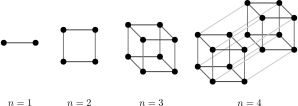
\includegraphics[width =
  0.8\linewidth]{./img/sos-dp/hypercube/Dimension_levels.pdf}
\end{figure}

যেমন, আমাদের আগের আলোচনায় 1D অ্যারের ক্ষেত্রে $n=2$ কিংবা 2D অ্যারের ক্ষেত্রে
$(n,m) = (2,2)$, এমনকি 3D অ্যারের ক্ষেত্রে $(\mathtt{lim_x}, \mathtt{lim_y},
\mathtt{lim_z}) = (2,2,2)$ হলে সেগুলো একেকটি হাইপারকিউব হয়ে যেত।

প্রতিটা $n$ লেংথের বিটমাস্ককে আমরা $n$-ডাইমেনশনের হাইপারকিউবের একটি ``সেল''
বলতে পারি। আর এভাবে যদি একটি বিটমাস্ককে একটি সেল হিসেবে ডিফাইন করি, তাহলে
খেয়াল করবে, সেই বিটমাস্কের প্রতিটি সাবসেট হলো হাইপারকিউবের মধ্যে $(0, 0,
\ldots, 0)$ পয়েন্ট থেকে ওই বিটমাস্কের পয়েন্ট পর্যন্ত সব সেল বা vertex এর
একটি। অর্থাৎ, একটি হাইপারকিউব $f$ এর প্রিফিক্স সামের হাইপারকিউব হলো $\hat{f}
= \zeta(f)$। 2D বা 3D এর মতো একইভাবে $n$-ডাইমেনশনের জন্যও আমরা প্রিফিক্স সাম
ক্যাল্কুলেট করতে পারি। নিচে কমেন্ট সহ এর \texttt{C++} কোড দেওয়া হলো:
\begin{lstlisting}[language=C++]
for(int i = 0; i < n; ++i) { // iterate on the dimensions
  for(int mask = 0; mask < (1 << n); ++mask) { // iterate over all the points
    if(mask >> i & 1) {
      /* similar to g[i][j][k] += g[i-1][j][k], g[i][j][k] += g[i][j-1][k],
       * and g[i][j][k] += g[[i][j][k-1] */
      f[mask] += f[mask - (1 << i)];
    }
  }
}
// we have applied zeta transformation on f; now fhat[x] = f[x]
\end{lstlisting}

\section{M{\"o}bius Inversion}
এককথায়, $\zeta^{-1}(\hat{f})$ বা $\mu(\hat{f}) = f$। আমাদেরকে
$\hat{f}$ দেওয়া থাকলে এমন
একটা $f$ ক্যাল্কুলেট করতে হবে যেন $\zeta(f) = g$ হয়। $\hat{f} \mapsto f$ এই
ট্রান্সফরমেশনকেই M{\"o}bious inversion বলা হয়। যেহেতু এটাকে M{\"o}bius
inversion বলা হচ্ছে, তাই zeta transform-কে M{\"o}bius transform-ও বলা যায়।

প্রথম প্রশ্ন হলো আমরা কি আসলেই এমন ফাংশন বের করতে পারবো কিনা, বা পারলেও
সবসময়ই পারবো কিনা। এটা বুঝার জন্য একটা উপায় হলো লিনিয়ার অ্যালজেব্রার ভাষায়
চিন্তা করা। ফাংশন $f$ কে আমরা একটি $2^n \times 1$ সাইজের কলাম ভেক্টর
$\vec{f}$ দিয়ে প্রকাশ করতে পারি, যেখানে 
\[
  \vec{f} =
  \begin{pmatrix}
    f\one{0}\\
    f\one{1}\\
    \vdots\\
    f\one{2^n-1}
  \end{pmatrix}
\]
একইভাবে $\hat{f}$ কে কলাম ভেক্টর $\vec{\hat{f}}$ দিয়ে প্রকাশ করা যাবে।
এবার খেয়াল করলে দেখবে, $\vec{f} \mapsto \vec{\hat{f}}$ একটি লিনিয়ার
ট্রান্সফরমেশন। এর
ট্রান্সফরমেশন ম্যাট্রিক্স $\zeta$ কে আমরা এভাবে সংজ্ঞায়িত করতে পারি:
$\zeta\two{x}{y} = 1$ যদি $y \subseteq x$ হয়, নাহলে $\zeta\two{x}{y} = 0$।
তাহলে,
\[
  \vec{\hat{f}} = \zeta \vec{f}
\]
এই ট্রান্সফরমেশন ম্যাট্রিক্স $\zeta$ এর ইনভার্স ম্যাট্রিক্স $\zeta^{-1} =
\mu$ বিদ্যমান
(invertible), কারণ খেয়াল করলে দেখবে $\zeta$ একটি lower triangular
ম্যাট্রিক্স যার diagonal-এ সব $1$। সুতরাং আমরা বলতে পারি, প্রত্যেক ফাংশন
$\hat{f}$ এরই M{\"o}bius inversion আছে।
\[
  \vec{f} = \zeta^{-1}\vec{\hat{f}} = \mu\vec{\hat{f}}
\]

এটা ছাড়াও অন্য একভাবে zeta transform এর ইনভার্স কেন আছে তা ব্যাখ্যা করতে
পারি। আগের সেকশনে আমরা zeta transform এর কোড দেখেছি, যেটা $f$-এর উপর
কিছু ম্যাথম্যাটিক্যাল অপারেশন অ্যাপ্লাই করে সেটাকে $\hat{f}$ তে রূপান্তর
করেছে। $n$-বিটের বিটমাস্কের ফাংশন $f$ এর zeta transform কে আমরা $n \cdot
2^{n-1}$ টা বিটমাস্কের পেয়ার দিয়ে প্রকাশ করতে পারি:
\begin{center}
  $(x_1, y_1)$\\
  $(x_2, y_2)$\\
  $\vdots$\\
  $(x_{n 2^{n-1}}, y_{n 2^{n-1}})$
\end{center}
যার মানে হলো নিচের অপারেশন গুলো ক্রমান্বয়ে $f$ অ্যারের উপর অ্যাপ্লাই করা:
\begin{center}
  $\mathtt{f[x_1] := f[x_1] + f[y_1]}$\\
  $\mathtt{f[x_2] := f[x_2] + f[y_2]}$\\
  $\vdots$\\
  $\mathtt{f[x_{n 2^{n-1}}] := f[x_{n 2^{n-1}}] + f[y_{n 2^{n-1}}]}$
\end{center}
যেহেতু যোগ (+) অপারেটরের ``ইনভার্স'' অপারেটর (-) আছে, এবং এই লিস্টে সব $i$ এর
জন্যই $x_i \ne y_i$, তাই আমরা এই লিস্টের ইনভার্স লিস্ট লিখতে পারবো:
\begin{center}
  $\mathtt{f[x_{n 2^{n-1}}] := f[x_{n 2^{n-1}}] - f[y_{n 2^{n-1}}]}$\\
  $\mathtt{f[x_{n 2^{n-1} - 1}] := f[x_{n 2^{n-1} - 1}] - f[y_{n 2^{n-1} -
  1}]}$\\
  $\vdots$\\
  $\mathtt{f[x_1] := f[x_1] - f[y_1]}$
\end{center}
এখান থেকে আশা করি বুঝতে পারছো zeta transforma এর কোডের লুপ গুলোকে উল্টা
অর্ডারে লিখলেই আমরা আবার $f$ পেয়ে যাবো!
\begin{lstlisting}[language=C++]
for(int i = n-1; i >= 0; --i) {
  for(int mask = (1 << n) - 1; mask >= 0; --mask) {
    if(mask >> i & 1) {
      fhat[mask] -= fhat[mask - (1 << i)];
    }
  }
}
// we've inverted fhat; now f[x] = fhat[x]
\end{lstlisting}

\section{সেট দিয়ে Zeta Transform-এর ব্যাখ্যা এবং M{\"o}bius Inversion এর ফর্মুলা}
Zeta transform-এর সাবসেটকে পরিবর্তন করে সুপারসেট করে দিয়ে আমরা
$\zeta_{\supseteq}$-transform ডিফাইন করলাম ধরো। অর্থাৎ, $\hat{f} =
\zeta_{\supseteq}(f)$, যেখানে
\[
  \hat{f}\one{x} = \sum_{y \supseteq x} f\one{y}
\]
আমরা $\zeta$-transform এবং $\zeta$-inversion (M{\"o}bius inversion) নিয়ে কথা
না বলে $\zeta_{\supseteq}$-transform এবং তার সংশ্লিষ্ট ইনভার্শন নিয়ে আলোচনা
করবো এই সেকশনে, কারণ ২টা জিনিসই একটা থেকে আরেকটায় কনভার্ট করা যায়।

ধরো তোমার কাছে $n$-টা সেট $A_0, A_1, \ldots, A_{n-1}$ আছে। আমরা বর্ণনার
সুবিধার্থে একটি নোটেশন ডিফাইন করে নেওয়া যাক -- $N$ এর সব সাবসেট
$J$ এর জন্য $A_J$ হলো $J$-তে যেই ইনডেক্স গুলো আছে,
সেই সেট গুলোর ইন্টারসেকশন। অর্থাৎ,
\[
  A_J = \bigcap_{j \in J} A_j
\]
বিশেষ করে $A_\emptyset = \emptyset$।
এবার আমরা $A_i$ গুলোকে এমন ভাবে ডিফাইন করবো যেন সেগুলো সব $J
\subseteq N$ এর জন্য নিচের শর্তটি পূরণ করে:
\begin{bigcondition}
  ধরো $t$ হলো এমন সব উপাদানের সংখ্যা, যেগুলো এমন সব সেট $A_j$ এর
  প্রত্যেকটিতেই আছে যেখানে $j \in J$ কিন্তু এমন সব সেট $A_j$ এর
  একটিতেও নেই যেখানে $j \ne J$। অনেকটা
  এভাবে বলা যায়: ``যেসব উপাদান বিশেষভাবে শুধুমাত্র $A_j$ সেট গুলোতেই আছে,
  যেখানে $j \in J$''। সেট থিওরির ভাষায় বললে হয়:
  \[
    t = \abs{ \pbra{\bigcap_{j \in J} A_j} \setminus
    \pbra{\bigcup_{j \ne J} A_j} }
  \]

  $t$ এর মান $f\one{J}$ এর সমান হতে হবে।
\end{bigcondition}

সেটগুলোর ভেন ডায়াগ্রামের আর কিছু জিনিস ডিফাইন করে নেয়াও যাক। কোন একটা $J
\subseteq N$ এর জন্য ভেন ডায়াগ্রামে $\mathcal{R} = \abs{ \pbra{\bigcap_{j \in
J} A_j}
\setminus \pbra{\bigcup_{j \ne J} A_j} }$ যেই অঞ্চলটুকু দখল করবে সেটাকে আমরা
একটা ফেস (face) বলবো। একটা উল্লেখযোগ্য বৈশিষ্ট্য হলো ফেস গুলো ডিসজয়েন্ট
(disjoint), অর্থাৎ ২টি ফেস-এর মধ্যে কোন সাধারণ উপাদান নেই। ফেস বলার কারণ
হচ্ছে, যেকোনো সংখ্যক সেটের জন্য ভেন ডায়াগ্রাম এমন ভাবে আঁকা সম্ভব যাতে
$\mathcal{R}$ এর
অঞ্চলটা আবদ্ধ এবং কানেক্টেড হয়। 2D প্লেন-এ এমন অঞ্চলকে ফেস বলা হয়।

চিত্র \ref{two_f_example}-এ $f_{\{0, 2\}}$, $f_{\{1,2,3\}}$ এবং
$f_{\{3\}}$ এর এলাকাকে ছায়া দিয়ে লেবেল করে দেখানো হয়েছে।
\begin{figure}[!ht]
  \centering
  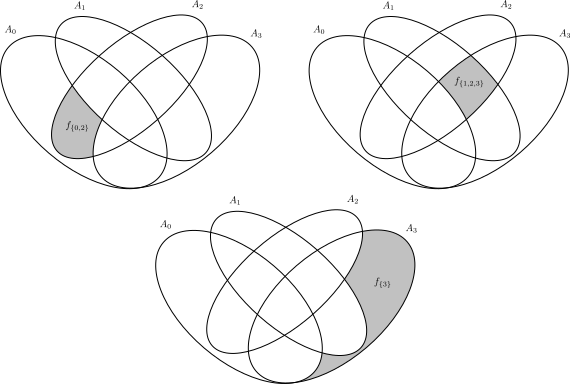
\includegraphics[width=\textwidth]{./img/sos-dp/4set/two_f_example.pdf}
  \caption{$A_0, A_1, A_2, A_3$ এর সংজ্ঞা অনুযায়ী কয়েকটি $J$ এর জন্য
  $f\one{J}$ এর উদাহরণ।}
  \label{two_f_example}
\end{figure}

\subsection{Zeta Transform}
ধরো আমরা $\hat{f}_{\{0,3\}}$ এর মান বের করতে চাচ্ছি। তাহলে যেটা হবে তা
চিত্র \ref{fhat_03_sum}-তে দেখানো হলো:
\begin{figure}[!ht]
  \centering
  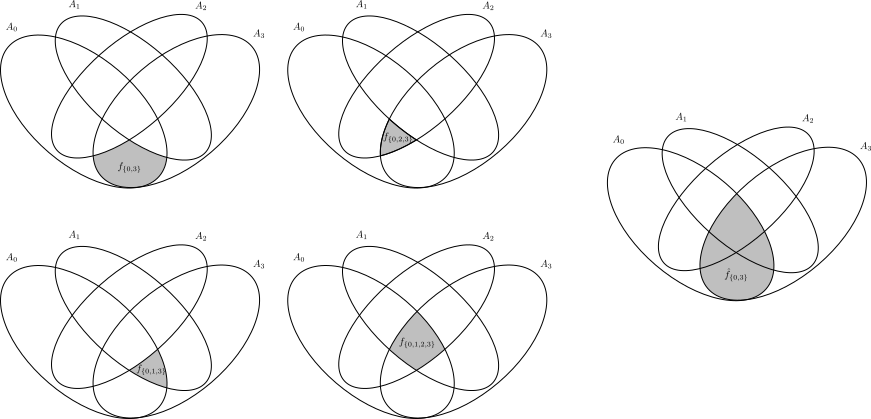
\includegraphics[width=\textwidth]{./img/sos-dp/4set/fhat_03_sum.pdf}
  \caption{$\hat{f}_{\{0,3\}} = f_{\{0,3\}} + f_{\{0,1,3\}} +
  f_{\{0,2,3\}} + f_{\{0,1,2,3\}}$}
  \label{fhat_03_sum}
\end{figure}
$\hat{f}_{\{0,3\}} = A_0 \cap A_3$ পাওয়া যায়! আর কয়েকটা এভাবে একে দেখলে
বুঝতে পারবে সব $J$ এর জন্য $\hat{f}\one{J} = \abs{\bigcap_{j \in J} A_j}$ হয়।
চিত্র \ref{three_fhat_example}-এ এমন আর কয়েকটি $\hat{f}\one{J}$ এর উদাহরণ
দেখানো হয়েছে।
\begin{figure}[!ht]
  \centering
  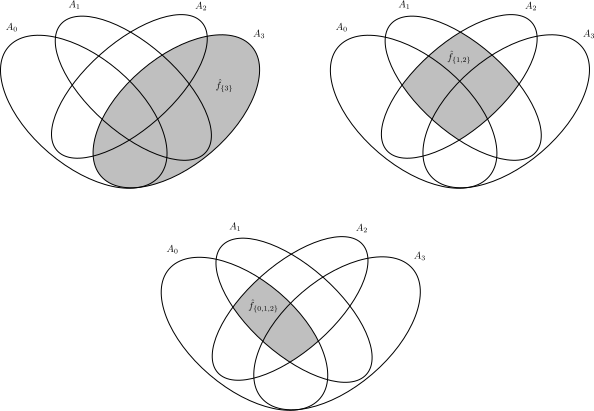
\includegraphics[width%
  =\textwidth]{./img/sos-dp/4set/three_fhat_example.pdf}
  \caption{কয়েকটি $\hat{f}\one{J}$ এর উদাহরণ}
  \label{three_fhat_example}
\end{figure}
সুতরাং, $\zeta_\supseteq$-transform হলো:
\begin{gather*}
  f\one{J} = \abs{ \pbra{\bigcap_{j \in J} A_j} \setminus
  \pbra{\bigcup_{j \ne J} A_j} }\\
  \rotatebox[origin = c]{-90}{$\xmapsto{\rotatebox[origin =
  c]{90}{$\zeta_\supseteq$}}$}\\
  \hat{f}\one{J} = \abs{ \bigcap_{j \in J} A_j }
\end{gather*}
অন্যভাবে বললে:
\[
  \text{face} \xmapsto{\zeta} \text{intersection of sets}
\]

\subsection{M{\"o}bius Inversion}
সেট এবং ফেস-এর ভাষায় m{\"o}bius inversion তাহলে হবে:
\[
  \text{intersection of sets} \xmapsto{\mu} \text{face}
\]

এখন যেহেতু আমরা বুঝতে পারছি zeta transform এর মাধ্যমে প্রতি $J$ এর জন্য
$f\one{J}$ venn diagram-এর কোন অংশ হতে ট্রান্সফর্ম হয়ে কোন অংশে যাচ্ছে, তাই
এটাকে কাজে লাগিয়ে আমরা $\hat{f}$ এর অংশগুলো থেকে $f$ এর অংশ গুলো বের করার
চেষ্টা করবো। মূলত এখন সমস্যাটা দাঁড়ালো এই:
\begin{reducedproblem}
  যদি প্রতিটি $J \subseteq N$ এর জন্য $\abs{ \bigcap_{j \in J} A_j }$ দেওয়া
  থাকে, তাহলে প্রতিটি $J \subseteq N$ এর জন্য $\abs{ \pbra{\bigcap_{j \in J}
  A_j} \setminus \pbra{\bigcup_{j \ne J} A_j} }$ ক্যাল্কুলেট করতে হবে।
\end{reducedproblem}
এটা খুব সহজেই প্রিন্সিপাল অফ ইনক্লুশন-এক্সক্লুশন দিয়ে করা যায়। যেমন,
যদি $n=4$ এর ক্ষেত্রে $f_{\{0,2\}}$ ক্যল্কুলেট করতে চাই তাহলে প্রথমেই
$\hat{f}_{\{0,2\}}$ কে আমাদের যোগফলে যোগ করবো। এরপর $\hat{f}_{\{0,2\}}$ থেকে
$f_{\{0,2,3\}}$, $f_{\{0,1,2\}}$, $f_{\{0,1,2,3\}}$ গুলো বাদ দেওয়ার জন্য
$\hat{f}_{\{0,1,2\}}$ এবং $\hat{f}_{\{0,2,3\}}$ বিয়োগ দিবো। কিন্তু এরপর আবার
$f_{\{0,1,2,3\}}$ একবার বেশি বিয়োগ হয়ে গিয়ে থাকবে। সেটা ঠিক করার জন্য আবার
$\hat{f}_{\{0,1,2,3\}}$ যোগ করতে হবে। সব মিলিয়ে হবে:
\begin{figure}[!ht]
  \centering
  \includegraphics[width = \textwidth]{./img/sos-dp/4set/inc_exc.pdf}
\end{figure}
\[
  f_{\{0,2\}} = \hat{f}_{\{0,2\}} - \hat{f}_{\{0,1,2\}} - \hat{f}_{\{0,2,3\}}
  + \hat{f}_{\{0,1,2,3\}}
\]
সাধারণ ভাবে বললে:
\[
  f\one{X} = \sum_{Y \supseteq X} (-1)^{\abs{Y \setminus X}} \hat{f}\one{Y}
\]
এটাই $\mu_\supseteq$-inversion ফর্মুলা! এটাকে এভাবেও দেখতে পারো: $A_X$ হলো
ইউনিভার্সাল সেট, আর $A_Y$ (যেখানে $Y \supset X$ এবং $|Y| = |X|+1$) গুলো হলো
প্রাইমারি সেটসমূহ। এখন, $f\one{X}$ বের করতে চাওয়ার মানে হলো প্রাইমারি
সেটগুলোর ইউনিয়নের কমপ্লিমেন্ট বের করা।

অনুরূপভাবে $\mu_\subseteq$ বা
ক্লাসিক্যাল M{\"o}bius inversion ফর্মুলা হবে:
\[
  f\one{X} = \sum_{Y \subseteq X} (-1)^{\abs{X \setminus Y}} \hat{f}\one{Y}
\]

\section{ফাস্ট সাবসেট কনভল্যুশন (Fast Subset Convolution)}
দুটি ফাংশন $f$ এবং $g$ দেওয়া থাকলে এদের subset convolution $(f * g)$-কে
ডিফাইন করা হয় এভাবে:
\[
  (f*g)\one{S} = \sum_{T \subseteq S} f\one{T}g\one{S \setminus T}
\]
অথবা অন্যভাবে লিখলে:
\begin{align*}
  (f * g)\one{S} &= \sum_{\substack{U,V \subseteq S \\ U \cup V = S \\ U \cap
  V = \emptyset}} f\one{U} g\one{V}\\
  &= \sum_{\substack{U,V \subseteq S \\ U \cup V = S \\ |U| + |V| = |S|}}
  f\one{U} g\one{V}
\end{align*}
2006 সালে \citet{10.1145/1250790.1250801} একটি পেপার পাবলিশ করেন যেখানে
তারা $O(n^2 2^n)$ কমপ্লেক্সিটিতে সাবসেট কনভল্যুশন বের করার একটা উপায় দেখান।
এই সেকশনে সেটা নিয়েই আলোচনা করা হবে।

প্রথমেই কিছু প্রয়োজনীয় ফাংশন ডিফাইন করে নেওয়া যাক। $f$ এর র‍্যাঙ্কড
M{\"o}bius transform $\hat{f}\two{i}{S}$ কে এভাবে সংজ্ঞায়িত
করা হলো:
\[
  \hat{f}\two{i}{S} = \sum_{\substack{T \subseteq S\\|T|=i}} f\one{T}
\]
যেখানে $i = 0, 1, 2, \ldots, n$ এবং $S \subseteq N$। একইভাবে
$\hat{g}\two{i}{S}$ সংজ্ঞায়িত করা হলো।

এবার কিছুটা অদ্ভুত একটা ফাংশন $p_k\one{S}$ সংজ্ঞায়িত করবো (যেখানে $i =
0,1,2,\ldots n$ এবং $S \subseteq N$):
\[
  p_k\one{S} = \sum_{\substack{U, V \subseteq S\\U \cup V = S\\|U| + |V| =
  k}} f\one{U} g\one{V}
\]
একটু অদ্ভুত হলেও কিছুক্ষণ পরেই বুঝতে পারবা এটা কতটা পাওয়ারফুল একটা ফাংশন।
বিশেষ করে, আমরা কিন্তু এখানে বলে দেইনি $U$ আর $V$ ডিসজয়েন্ট (disjoint) হতে
হবে; এরা ওভারল্যাপ করতে পারে, এটা খেয়াল রেখো। আরেকটি খেয়াল করার বিষয় হলো
$p_|S|\one{S} = (f*g)\one{S}$। ডেফনিশনটাকে একটু অন্যভাবে
লিখলে হবে:
\[
  p_k\one{S} = \sum_{i=0}^{k} \sum_{\substack{U \subseteq S\\|U|=i}} \sum_{\substack{V \subseteq S\\|V|=k-i\\U \cup V = S}} f\one{U} g\one{V}
\]

পেপারটিতে দেখানো হয়েছে র‍্যাঙ্কড মোবিয়াস ট্রান্সফর্ম গুলো ব্যবহার করে সহজেই
প্রতি $k$ এর জন্য $p_k$ এর zeta/m{\"o}bius transform $\hat{p_k}$ ক্যাল্কুলেট
করে নেওয়া যায়। আর এর পর শুধু $\hat{p_k}$ এর m{\"o}bius inversion নিলেই কাজ
শেষ।
\begin{align*}
  \hat{p_k}\one{S} &= \sum_{T \subseteq S} p_k\one{T}\\
  &= \sum_{T \subseteq S} \sum_{i=0}^{k} \sum_{\substack{U \subseteq
  T\\|U|=i}} \sum_{\substack{V \subseteq T\\|V|=k-i\\U \cup V = T}} f\one{U}
  g\one{V}\\
  &= \sum_{i=0}^{k} \sum_{T \subseteq S} \sum_{\substack{U \subseteq
  T\\|U|=i}} \sum_{\substack{V \subseteq T\\|V|=k-i\\U \cup V = T}} f\one{U}
  g\one{V}\\
  &= \sum_{i=0}^{k} \sum_{\substack{U \subseteq S\\|U| = i}}
  \sum_{\substack{V \subseteq S\\|V|=k-i}} f\one{U} g\one{V}\\
  &= \sum_{i=0}^{k} \pbra{\sum_{\substack{U \subseteq S\\|U| = i}} f\one{U}}
  \pbra{\sum_{\substack{V \subseteq S\\|V|=k-i}} g\one{V}}\\
  &= \sum_{i=0}^{k} \hat{f}\two{i}{S} \cdot \hat{g}\two{k-i}{S}
\end{align*}

প্রতি $i$ এর জন্য $\hat{f}\two{i}{\dots}$ এবং $\hat{g}\two{i}{\dots}$
ক্যাল্কুলেট করতে $O(n 2^n)$ টাইম লাগবে। সুতরাং সব $i$ এর জন্য মোট টাইম লাগবে
$O(n^2 2^n)$। এরপর $\hat{f}$ এবং $\hat{g}$ থেকে $\hat{p_k}$ ক্যাল্কুলেট করতে
$O(n^2 2^n)$ কমপ্লেক্সিটি লাগবে। সব শেষে, সব $k$ এর জন্য $p_k$ এর m{\"o}bius
inversion নিতে মোট সময় লাগবে $O(n^2 2^n)$। তাই এই অ্যালগরিদমের কমপ্লেক্সিটি
হলো $O(n^2 2^n)$। নিচে এটির \texttt{C++} কোড দেওয়া হলো:
\begin{lstlisting}[language=C++]
// given f[], g[], find fg[]
// initialize fhat[][] and ghat[][] with 0s
for(int mask = 0; mask < (1 << n); ++mask) {
  fhat[__builtin_popcount(mask)][mask] = f[mask];
  ghat[__builtin_popcount(mask)][mask] = g[mask];
}
// calculate ranked mobius transforms of f and g
for(int i = 0; i <= n; ++i) {
  for(int j = 0; j < n; ++j) {
    for(int mask = 0; mask < (1 << n); ++mask) {
      if(mask >> j & 1) {
        fhat[i][mask] += fhat[i][mask - (1 << j)];
        ghat[i][mask] += ghat[i][mask - (1 << j)];
      }
    }
  }
}
// initialize phat[][] with 0s
for(int k = 0; k <= n; ++k) {
  for(int mask = 0; mask < (1 << n); ++mask) {
    for(int i = 0; i <= k; ++i) {
      phat[k][mask] += f[i][mask] * g[k-i][mask];
    }
  }
}
// take mobius inversion of phat[k][] for each k
for(int k = 0; k <= n; ++k) {
  for(int i = n-1; i >= 0; --i) {
    for(int mask = (1 << n) - 1; mask >= 0; --mask) {
      if(mask >> i & 1) {
        phat[k][mask] -= phat[k][mask - (1 << i)];
      }
    }
  }
}
// now, fg[mask] = phat[__builtin_popcount(mask)][mask]
\end{lstlisting}

\section{কিছু উদাহরণ}

\begin{example}[\href{https://atcoder.jp/contests/arc100/tasks/arc100_c}{Or
  Plus Max}]
  তোমাকে একটা $2^n$ লেংথের ইন্টিজার সিকুয়েন্স $A_0, A_1, \ldots,$ $A_{2^n-1}$
  দেওয়া আছে। প্রতিটা ইন্টিজার $k \, (1 \le k \le 2^n-1)$ এর জন্য ক্যাল্কুলেট
  করতে হবে: $A_i + A_j$ এর ম্যাক্সিমাম ভ্যালু, যেখানে $0 \le i < j \le 2^n-1$
  এবং $(i \, \texttt{|} \, j) \le k$। এখানে \texttt{|} দিয়ে বিটওয়াইজ অর
  বুঝানো হয়েছে। $1 \le n \le 18$, $1 \le A_i \le 10^9$।
\end{example}
\begin{solution}
  এই প্রবলেমের সলিউশনের যেই অবজারভেশনটা লাগবে আমাদের, তাহ হলো:
  \begin{observation}
    কোন সংখ্যা $x$ যদি $y$ এর চেয়ে ছোট অথবা সমান হয়, তাহলে সেটা কোন না কোন
    একটা সংখ্যা $z$ এর সাবমাস্ক যেখানে $z \le y$। অর্থাৎ,
    \[
      \forall x \forall y ((x \le y) \implies (\exists z (z \le y \land x
      \subseteq z)))
    \]
  \end{observation}
  এরপর আমাদের প্রবলেমটা দাঁড়ায়, প্রত্যেক $k$ এর জন্য ক্যাল্কুলেট করতে হবে:
  \begin{align*}
    g\one{k} &= \max_{\substack{(i\texttt{|}j) \subseteq k\\i \ne j}} A_i +
    A_j\\
    &= \max_{\substack{i, j \subseteq k\\i \ne j}} A_i +
    A_j
  \end{align*}
  যার মানে হলো $k$ সাবসেট গুলোর মধ্যে ম্যাক্সিমাম ২টা বের করতে হবে। এরপর $g$
  এর প্রিফিক্স ম্যাক্সিমাম নিয়ে নিলেই হয়ে যাবে। এটা করার জন্য আমরা zeta
  ট্রান্সফর্মের মতো কাজ করবো অনেকটা। $f$ ফাংশনটিকে একটা সেট/বিটমাস্ক দিলে
  সেটা একটা পেয়ার রিটার্ন করবে -- সবচেয়ে বড় ২টি সংখ্যা। শুরুতে $f\one{S} =
  \{A_S, -\infty\}$ থাকবে। এরপর $f$ এর উপর zeta transform অ্যাপ্লাই করতে হবে।
  আর ২টি পেয়ার $\texttt{a}$ এবং $\texttt{b}$ কম্বাইন করার সময়
  $\{\mathtt{a_{first}}, \mathtt{a_{second}}, \mathtt{b_{first}},
  \mathtt{b_{second}}\}$-এই মাল্টিসেটের সবচেয়ে বড় ২টি সংখ্যা নিতে হবে।
\end{solution}
% \begin{example} শুরুতে তোমার কাছে একটি $n$ লেংথের অ্যারে $A = [0, 0,
% \ldots, 0]$ আছে। তুমি এর উপর কিছু অপারেশন অ্যাপ্লাই করতে পারো। প্রতিটা
% অপারেশন হলো: প্রথমে $A$ এর একটি সাবঅ্যারে নির্বাচন করবা, তারপর সেই
% সাবঅ্যারেতে তোমার পছন্দের একটি ধনাত্মক পূর্ণসংখ্যা যোগ করে দিবা। তোমাকে বের
% করতে হবে, মিনিমাম কয়টি অপারেশন অ্যাপ্লাই করে $A$ অ্যারেটিকে তুমি আরেকটি
% প্রদত্ত অ্যারে $B$ এর সমান বানাতে পারবে। $n \le 20$, $1 \le B_i \le 10^9$।
% \end{example}
\begin{example}[\href{https://olymp.innopolis.ru/ooui/informatics/upload/%
  2018-2019/inno-2019-final-en.pdf}{Innopolis Open 2019 - Cake Testing}]
  কারিনা কেক খুব পছন্দ করে। তার শহরে $n$ টি কেকের দোকান আছে। সে মোট $2^n-1$
  দিন ঘর থেকে বের হবে। দিন গুলো $1, 2, \ldots, 2^{n}-1$ নিয়ে নাম্বারিং করা,
  এবং দোকান গুলো $0, 1, \ldots, n-1$ দিয়ে। $i$ তম দিনে বের হলে সে $j$-তম
  দোকানে যাবে যদি $i$-এর বাইনারিতে $j$-তম বিট অন থাকে। কোন দোকানে গেলে সে
  দোকানে থাকা সব টাইপের কেক একটি করে খায়। অবশ্য একই টাইপের কেক একাধিক দোকানে
  থাকতে পারে। দিন শেষে সে নোট করে, সারাদিনে সে কয়টা ভিন্ন ভিন্ন টাইপের কেক
  খেয়েছে (একই টাইপের কেক একাধিক দোকানে খেয়ে থাকলেও একবারই হিসাবে যোগ হবে)।
  $i$-তম দিনের জন্য এই সংখ্যাটি হলো $a_i$। তোমাকে যাচাই করতে হবে $a_i$ এর
  ভ্যালু গুলো সামঞ্জস্যপূর্ণ কিনা। অর্থাৎ, আমরা যদি $i$-তম দোকানে পাওয়া যায়
  এমন কেকের টাইপগুলোর সেটকে $S_i$ দিয়ে প্রকাশ করি যেখানে $S_i$ হলো স্বাভাবিক
  সংখ্যার সেট, তাহলে তোমাকে বের করতে হবে
  এমন কোনো সেটের সিকুয়েন্স $\bbra{S_1, S_2, \ldots, S_{2^n-1}}$ আছে কিনা
  যেগুলো প্রতি $\mathtt{mask}$ এর জন্য নিচের শর্ত মেনে চলে:
  \begin{equation}
    \label{inno19finalsoscondition}
    \abs{\bigcup_{j,\, \mathtt{mask_j} = 1} S_j} = a_i
  \end{equation}
  যদি থেকে থাকে, তাহলে এমন একটি সেটের সিকুয়েন্স প্রিন্ট করতে হবে। $n \le 19$,
  $1 \le a_i \le 1000$।
\end{example}
\begin{solution}
  ধরো ইউনিভার্সাল (universal) সেট $U = \bigcup_{i=1}^{2^n-1} S_i$। প্রথমেই
  খেয়াল করো, ডি মরগানের ল' ব্যবহার করে আমরা
  \ref{inno19finalsoscondition}-শর্তের সেট ইউনিয়ন গুলোকে সেট ইন্টারসেকশন
  বানিয়ে ফেলতে পারি। অর্থাৎ,
  \[
    \abs{\bigcup_{j,\, \mathtt{mask_j} = 1} S_j} = a_i \Leftrightarrow
    \abs{\bigcap_{j,\, \mathtt{mask_j} = 1} \compl{S_j}} = \compl{a_i}
  \]
  যেখানে $\compl{a_i} = |U| - a_i$। অন্যদিকে, কিছু সেটের সবরকম ইন্টারসেকশনের
  সাইজ দিয়ে দেওয়া মানে একটা ফাংশনের zeta transform দেওয়া আছে, আর সেটার উপর
  m{\"o}bius inversion অ্যাপ্লাই করে আমরা সেটগুলোর ভেন ডায়াগ্রামের $2^n$-
  টা বিচ্ছিন্ন (disjoint) ফেস (face) এর সাইজ বের করে ফেলতে পারি। আবার প্রতিটা সেট সেসব disjoint face এর ইউনিয়ন। সুতরাং প্রতিটা
  disjoint face এর সাইজ বের করে ফেলতে পারলে সেগুলোতে সুবিধা মতো স্বাভাবিক
  সংখ্যা বাছাই করে দিতে পারবো এবং সহজেই $\compl{S_i}$ গুলো বের করে ফেলা যাবে।
\end{solution}
\begin{example}[\href{https://hsin.hr/coci/archive/2011_2012/%
  contest6_tasks.pdf}{Generalization of COCI - Kosare}]
  $N$ লেংথের একটা ইন্টিজার অ্যারে $a$ দেওয়া আছে, যেখানে $n \le 10^6$, $0 \le
  a_i < 2^{20}$। প্রত্যেক সংখ্যা $k$ এর জন্য তোমাকে বের করতে হবে $a$ এর এমন
  কয়টা সাব-সিকুয়েন্স আছে যেগুলোর or-sum $k$।
\end{example}
\begin{solution}
  ধরো $c\one{x}$ হলো $a$ তে $x$ কয়বার আছে তার সংখ্যা। $\hat{c} = \zeta(c)$
  হলে $\hat{f}\one{x} = 2^{\hat{c}\one{x}}$ হলো এমন কয়টা সাব-সিকুয়েন্স আছে,
  যাদের or-sum $x$ এর সাবমাস্ক। ধরো $f\one{x}$ হলো এমন কয়টা সাবসিকুয়েন্স আছে,
  যাদের or-sum বরাবর $x$। তাহলে খেয়াল করলে দেখবে, $\hat{f} = \zeta(f)$।
  $\mu(\hat{f})$ বের করলেই আমরা অ্যান্সার পেয়ে যাবো।
\end{solution}
\begin{example}[\href{http://www.usaco.org/index.php?page=%
  viewproblem2&cpid=129}{USACO 2012 - Skyscraper}]
  $n$ টা গরু আছে নিচতলায়, সবচেয়ে কম সংখ্যক বার লিফট ব্যবহার করে তাদেরকে উপর
  তলায় নিতে হবে। $i$-তম গরুর ওজন হচ্ছে $w_i$ নিউটন, আর লিফটের ক্যাপাসিটি
  হচ্ছে $W$ নিউটন। $n \le 18$, $w_i \le W$, $W \le 100\,000\,000$।
\end{example}
\begin{solution}
  $3^n$ সলিউশন: $\DP\one{S}$, যার মানে হলো $S$-এ
  থাকা গরুগুলো লিফট দিয়ে উঠাতে মিনিমাম কয়বার লিফট ব্যবহার করতে হবে।
  রিকার্শন হলো:
  \[
    \DP\one{S} = \min_{\substack{T \subseteq S\\T \ne \emptyset\\\sum_{i \in
    T} w_i \le W}} \DP\one{S \setminus T} + 1
  \]

  একটু অন্যভাবে চিন্তা করলে এরকম কিছু করতে পারি: স্টেটে থাকবে কোন কোন গরু
  বাকি আছে সেটার সেট, আর বর্তমানে যেই গরুর ব্যাচ খোলা হয়েছে সেটার ওজনের
  যোগফল। এগুলো মাথায় রেখে বাকি গরুগুলো মিনিমাম কয়টা ব্যাচে ভাগ করা যায়।
  কিন্তু এভাবে করতে গেলে আবার $O(2^n n W)$ কমপ্লেক্সিটি টাইপের কিছু হয়ে যাবে।
  
  এখন আমরা ডিপির স্টেট-ভ্যালু সোয়াপের ট্রিক ব্যবহার করবো:
  $\hat{f_i}\one{S}$ দিয়ে বুঝানো হবে: $i$ টা লিফটের মধ্যে আমরা গরুগুলো
  পাঠানোর চেষ্টা করবো,
  কিন্তু যদি না পারি তাহলে বাকি যেই গরু গুলো থেকে যাবে তাদের ওজনের যোগফল যেন
  সর্বোনিম্ন হয়। আরেক্টু গুছিয়ে বললে হবে, এর মান $\sum_{i \in S} w_i$ হবে যদি
  $i$ টা লিফট-রাইড দিয়েই $S$ এর সব গরুকে উপরে পাঠাতে পারি। কিন্তু যদি না পারি
  তাহলে $\hat{f_i}\one{S}$ এর মান হবে $\sum_{i \in T} w_i$ যেখানে $T$ হলো $S$
  এর এমন একটা সাবসেট যাতে $T$ এর সব গরুকে $i$ টা লিফট-রাইড দিয়েই উপরে উঠানো
  সম্ভব।

  ধরো আমরা $f_i\one{S}$ কে এমন ভাবে ডিফাইন করি যাতে $f_i\one{S} = 0$ যদি $S$
  কে $i$ টা লিফট-রাইড দিয়ে উঠানো সম্ভব না হয়, আর $f_i\one{S} = \sum_{i \in
  S} w_i$ যদি $i$-টা লিফট-রাইড যথেষ্ট হয়। একটু খেয়াল করলে দেখবা $\hat{f_i} =
  \zeta_{\max}(f_i)$, যেখানে $\hat{f} = \zeta_{\max}(f)$ এর মানে হলো:
  \[
    \hat{f}\one{X} = \max_{Y \subseteq X} f\one{Y}
  \]
  
  এরপর একটা সেট $S$ এর জন্য $i+1$-টা লিফট-রাইড যথেষ্ট কিনা চেক করার জন্য
  $\sum_{i \in S} w_i - \hat{f_i}\one{S} \le W$ কিনা চেক করলেই হবে।
\end{solution}
\begin{example}[\href{https://codeforces.com/contest/986/problem/C}%
  {Codeforce - AND Graph}]
  তোমাকে $m \, (1 \le m \le 2^n)$ সাইজের একটা সেট $A=\{a_1, a_2, a_3, \ldots,
  a_m\}$ দেওয়া আছে, যেখানে $0 \le a_i < 2^n$ এবং $n \le 22$। এই সেট থেকে তুমি
  $n$-টা নোডের একটা bidirectional গ্রাফ $G$ বানাবা, যেখানে নোডের সেট হলো $A$,
  এবং $u$ থেকে $v$ এর মধ্যে এজ থাকবে যদি এবং কেবল যদি $x \texttt{ \& } y = 0$
  হয়। $G$-তে কয়টা কানেক্টেড কম্পোনেন্ট আছে তা বের করতে হবে।
\end{example}
\begin{solution}
  আমরা যথারীতি Breadth First Search করবো। ধরো আমরা $u$ নোডে আছি। এমন সময় BFS
  অ্যালগরিদমে $u$ এর অ্যাডজেসেন্ট আনভিসিটেড নোড গুলো সব খুঁজে বের করে কিউ
  (queue)-তে ঢুকাতে হয়। এই অ্যাডজেসেন্ট আনভিসিটেড নোডগুলো বের করার সুবিধার্থে
  আমরা আরেকটি আন-ডাইরেক্টেড গ্রাফ $D$ বানাবো, যেটার ভার্টেক্স সেট হবে $\{(i,
  u) \, \mid \, i \in [1, n] \land u \in [0, 2^n-1]\} \cup \{(0, u) \, \mid
  \, u \in A\}$। এর মধ্যে $\{(0, u) \, \mid \, u \in A\}$-এর নোড গুলোকে আমরা
  ``টার্মিনাল নোড'' বলবো। এজ গুলো হবে এভাবে: সব $i \in [1, n]$ এবং $u \in [0,
  2^n - 1]$ এর জন্য $(i, u)$ থেকে $(i-1, u - 2^{i-1})$-এ ডাইরেক্টেড এজ দিব
  যদি $u$ এর $(i-1)$-তম বিট অন থাকে। $D$ গ্রাফের নোডগুলোর একটি সেট $S$ এর
  জন্য $\text{ter}(S) = \{u \, \mid \, (0, u) \in S\}$ দিয়ে $S$-এ থাকা
  টার্মিনাল নোডগুলোর সেটকে বুঝানো হবে।
  যদি $G$ গ্রাফে $u$ এর অ্যাডজেসেন্ট এবং আনভিসিটেড নোড গুলো পেতে চাই, তাহলে
  $D$ গ্রাফে $(n, u)$ থেকে রিচেবল (reachable) কিন্তু এখনো আনভিসিটেড (আবারও,
  $D$ তেই), এমন সব নোড DFS দিয়ে বের করবো। ধরো এইসব নোডের সেট হলো $R$। তাহলে
  $G$ গ্রাফে $u$ এর অ্যাডজেসেন্ট এবং আনভিসিটেড নোডের সেট হবে $\text{ter}(R)$।
  $D$ তে এই DFS চালানোর পর $R$ এর নোডগুলো $D$ তে ভিসিটেড (visited) করে দিতে
  হবে। মোট টাইম কমপ্লেক্সিটি $O(n 2^n)$।
\end{solution}
\section{অনুশীলনী}

\begin{exercise}[\href{https://www.codechef.com/SNFL16MR/problems/%
  BEAUTY}{Codechef - Beautiful Sandwich}]
  
\end{exercise}

\begin{exercise}[\href{https://www.codechef.com/problems/ANDPREF}{Codechef -
  Prefix And}]

\end{exercise}

\begin{exercise}[\href{https://codeforces.com/contest/1392/problem/G}{Omkar
  and Pies}]
  
\end{exercise}

\begin{exercise}[\href{https://codeforces.com/group/qcIqFPYhVr/contest/%
  203881/problem/K}{Pepsi Cola}]
  
\end{exercise}
% \begin{exercise}[\href{https://codingcompetitions.withgoogle.com/kickstart/%
%   round/0000000000050e02/000000000018fd5e\#problem}{Google Kickstart -
%   Shifts}]
% \end{exercise}

% \begin{exercise}[\href{https://codeforces.com/contest/449/problem/D}{Jzzhu
%   and Numbers}]
% \end{exercise}

\endgroup
% Include the chapters here

\Closesolutionfile{hint_ostream}

\part{বাছাইকৃত কিছু সমস্যার হিন্ট সমূহ}
\begin{Hint}{5.4.2}
প্রথম অভজারভেশন হলো, দুটো মাস $i$ এবং $j$ তে যদি তুমি ২টি অফার চালু করো (যেখানে $i < j$), তাহলে $i$ আর $j$ এর মধ্যে এমন কোন মাস $k$ থাকতে পারবে না যেটাতে তুমি কোন অফার চালু করোনি (অর্থাৎ, $i < k < j$ হতে পারবে না)। সুতরাং যেই মাসগুলোতে তুমি চালু করবা সেগুলো একটা consecutive রেঞ্জ হবে। ধরো তুমি একটা সিকুয়েন্স ঠিক করেছ $s_0, s_1, \ldots, s_{m-1} \, (m \le n)$, যার মানে হলো প্রথম মাসে তুমি $s_{m-1}$-তম অফারটি চালু করবে, দ্বিতীয় মাসে $s_{m-2}$-তম... $m$-তম মাসে $s_0$-তম অফারটি নিয়েছ, তাহলে এই সিকুয়েন্সের কস্ট হবেঃ
\[
  \sum_{i=0}^{m-1} a_{s_i} - b_{s_i} \cdot \min(k_{s_i}, i)
\]
এইরকম কস্ট ফাংশনে এক্সচেঞ্জ আর্গুমেন্ট অ্যাপ্লাই করতে ঝামেলা হবে, কারণ একটা $\min$ চলে এসেছে। সেজন্য আমরা এক কাজ করতে পারি, যেগুলোর জন্য $k_{s_i} < i$ হবে (অর্থাৎ, তুমি যখন গাড়ি নিয়ে পালিয়ে যাবে, তার আগেই এসব অফারের মেয়াদ শেষ হয়ে যাবে), সেগুলো পুরাপুরি আলাদা করে ফেলা। এদেরকে প্রথম টাইপের অফার বলবো এখন থেকে, আর বাকিগুলোকে দ্বিতীয় টাইপের অফার। এখন আরেকটা অভজারভেশন হলো, আমরা যদি প্রথম টাইপের অফার গুলো সব আগেভাগে নিয়ে ফেলি তাহলে আমাদের কোন লস হবে না। আরেকটা ক্রুশাল বিষয় হলো, এখন আমরা ধরে নিতে পারি প্রথম টাইপের অফার গুলা আমাদের মোট যোগফলে $a_i - b_i \cdot k_i$ কন্ট্রিবিউট করবে, আর এই জিনিসটা পুরাপুরি ইন্ডিপেন্ডেন্ট -- এই অফার কোন মাসে নেয়া হচ্ছে তার উপর নির্ভর করে না। কেন? এমন কি হতে পারে না যে এই অফারটিকে যখন চালু করেছিলাম তার পরে $k_i$ মাস পার হওয়ার আগেই তুমি গাড়ি নিয়ে পালিয়েছ? সেরকম হলে তো এই অফার আরও বেশি কন্ট্রিবিউট করতে পারতো! হতে পারে, কিন্তু যেটা খেয়াল করার বিষয় তা হলো, আমাদেরকে তো ম্যাক্সিমাম কস্ট বের করতে বলেছে। এমন যদি হয়, আমরা যেই ফিক্সড কন্ট্রিবিউশন ধরে নিয়েছি, তার কারণে আসল কস্টের চাইতে ডিপিতে কম অ্যাড হচ্ছে, তাহলে সেই সলিউশনটা অপ্টিমাল হবে না! চিন্তা করে দেখো এটা।

\noindent সুতরাং আমরা বলতে পারিঃ
\begin{gather*}
  \max_{s} \left ( \sum_{i=0}^{m-1} a_{s_i} - b_{s_i} \cdot \min(k_{s_i}, i) \right )\\
  = \max_{p \cap q = \emptyset} \left ( \sum_{i \in p} a_i - b_i \cdot k_i + \sum_{i=0}^{|q|-1} a_{q_i} - b_{q_i} \cdot i \right )
\end{gather*}
এখন আমাদের $q$ এর উপাদান গুলা কিভাবে সাজাতে হবে সেটা চিন্তা করতে হবে। এই কস্ট ফাংশনে এক্সচেঞ্জ আর্গুমেন্ট অ্যাপ্লাই করলে দেখবে উপাদান গুলো $b_i$ এর decreasing অর্ডারে সাজালে সবসময় অপ্টিমাল হবে। এরপর খালি একটা ডিপি লেখা বাকি আমাদের। শুরুতে সবকিছুকে $b_i$ দিয়ে বড় থেকে ছোট অর্ডারে সাজানোর পর বাম থেকে ডানে যাবা, একটা উপাদানের জন্য তিনটা অপশানঃ $p$ তে নিবা, $q$ তে নিবা, কোনটাতেই নিবা না। এছাড়াও, $q$ তে ইতোমধ্যে কয়টা নিয়ে ফেলেছ সেটাও স্টেটে রাখতে হবে।
\end{Hint}


% \backmatter

% \nocite{*}
% \bibliography{bookbib}
% \bibliographystyle{plain}

\end{document}
